% ============================================================
% wafer高次補正のアライメント計測shot選択における実務制約付き最適サンプリング（社内技術報告書）
% Overleaf: メニュー → Compiler を「LuaLaTeX」にしてコンパイルする
% 図は figures/ フォルダ（results/figures から報告書で使う図をコピーしたもの）を同じ階層に置く
% 数値は results/csv/*.csv（MATLAB の run_study で生成）から転記した
% ============================================================
\documentclass[10.5pt,a4paper]{ltjsarticle}
\usepackage{amsmath,amssymb,bm}
\usepackage{graphicx}
\usepackage{booktabs}
\usepackage{multirow}
\usepackage{array}
\usepackage{float}
\usepackage[margin=22mm]{geometry}
\usepackage[hidelinks]{hyperref}
\graphicspath{{figures/}}
\newcommand{\figw}{\textwidth}
\newcommand{\nm}{\,\mathrm{nm}}
\newcommand{\mm}{\,\mathrm{mm}}
\DeclareMathOperator*{\argmax}{arg\,max}
\DeclareMathOperator*{\argmin}{arg\,min}
\DeclareMathOperator{\tr}{tr}

\begin{document}

% ------------------------------------------------------------
% 表紙
% ------------------------------------------------------------
\begin{titlepage}
  \centering
  \vspace*{35mm}
  {\LARGE\bfseries wafer高次補正のアライメント計測shot選択における\\[3mm]実務制約付き最適サンプリング手法の構築と評価\par}
  \vspace{8mm}
  {\large ―象限・半径領域・scan方向・強制計測shotを統合したD/I最適計画と\\[1mm]optimal design augmentationの1000 wafer Monte Carlo評価―\par}
  \vspace{40mm}
  {\Large 著者名\par}  % ← 著者名を記入する
  \vspace{8mm}
  {\large \today\par}
  \vfill
  {\small 本報告の数値はすべて乱数で生成した模擬wafer（実データ・社内データは使用していない）による．\\
   未確定の工程パラメータは仮定値を置いており，表\ref{tab:assumptions}にまとめた．\par}
\end{titlepage}

\tableofcontents
\newpage

% ============================================================
\section{はじめに}
% ============================================================

\subsection{背景}

露光工程の重ね合わせ（overlay）精度を確保するため，露光装置は露光前にwafer上のalignment markの位置を計測し，wafer格子（shot配列）の変形を補正する．
古典的な方法は，選んだ数shot（sample shot）の位置から全shotの配列を一次変換で求めるEGA（Enhanced Global Alignment）である\cite{slonaker1988}．
その後，プロセス起因のwafer変形に対応するため，2次以上の多項式でwafer格子を表す高次補正が導入された\cite{adel2007}．
ASMLのHOWA（High Order Wafer Alignment）は3次以上の多項式に基づく公開手法と説明されており\cite{us9291916}，5次までのモデルを量産に適用した報告がある\cite{wang2009,pike2012,jeon2013}．

\subsection{wafer高次補正における計測shot選択の重要性}

高次補正では推定するパラメータが多い．
総次数$m$の2変数多項式の項数は$(m+1)(m+2)/2$で，3次で10項，4次で15項，5次で21項になり，X・Yで別々に推定する．
HOWAやRBFのような高度なモデルは数十のパラメータを持ち，多くのmark計測が必要になることが特許でも指摘されている\cite{us9291916}．
限られた計測shotでこれらを推定するとき，どのshotを測るかで，推定値のばらつき（計測誤差の増幅）と，モデルで表せない成分の写り込み（バイアス）が大きく変わる．
同じshot数でも，配置が悪ければ補正後の残差は大きくなり，極端な場合は推定そのものが不安定になる（説明変数行列がrank不足に近づく）．

\subsection{計測点数と補正精度のトレードオフ}

計測shotを増やせば補正精度は上がるが，露光装置内のalignment計測時間はスループットを直接下げる．
補正モデルと計測sampling schemeの組合せが歩留まりに影響することは量産データでも示されている\cite{chiu2012}．
近年は計測点が数百点に増えたことを受け，露光機外でalignment markを密に計測してfeed forwardする装置も登場している\cite{canon_ms001,nikon_litho_booster}．
しかし露光機内で計測できるshot数には上限があり，「少ないshotで，できるだけ小さい残差を得る」配置の設計は今も重要な課題である．

\subsection{本報告の目的}

本報告では，wafer高次補正用のalignment計測shot選択について，D最適計画・I最適計画をベースに，次の実務制約を満たす解空間の中で最適性を最大化（D）・最小化（I）する「実務制約付き最適サンプリング手法」を構築する．

\begin{itemize}
  \item wafer四象限ごとの計測数（象限制約）
  \item wafer半径方向の領域ごとの計測数（半径領域制約）
  \item scan方向（Up/Down）ごとの計測数（scan方向制約）
  \item 必ず計測しなければならないshot（強制計測shot）
  \item wafer外周のpartial shotは計測対象外（候補から除外）
  \item 1 shotあたり4個のalignment markを同時に計測する（最適化の単位はshot）
\end{itemize}

強制計測shotがある場合は，固定shotが既に持つ情報量を考慮して残りのshotを最適化する拡張実験計画（optimal design augmentation）として扱う．
手法の有効性は，数学的な最適性ではなく，乱数で生成した1000枚のwaferに対してHOWA型の高次補正を実際に適用した後の残差（Residual RMSとtail）と，同じ残差を得るのに必要な計測shot数で判断する．
D最適・I最適計画そのものは既存技術であり，本報告の新規性ではない（\ref{sec:prior-issues}節）．

% ============================================================
\section{対象技術と従来技術}
% ============================================================

\subsection{wafer高次補正の概要}

wafer上の位置$(x,y)$でのalignment計測値（設計位置からのずれ）$(d_x,d_y)$を，wafer全体で定義した関数で近似し，その関数で各shotの露光位置を補正する．
EGAではこの関数が一次変換（並進・倍率・回転・直交度）で，6〜数個のsample shotから全shotの配列を決める\cite{slonaker1988}．
EGAにはsample shotの位置に応じて重みを変える改良もある\cite{us5493402}．
高次補正では関数を2次以上の多項式に広げ，プロセスで生じるwafer面内の非線形な変形を補正する\cite{adel2007}．

\subsection{ASML HOWAをモチーフとした高次補正モデル}
\label{sec:howa}

本報告では，ASML製品の内部アルゴリズムの再現ではなく，公開情報\cite{us9291916,wang2009,pike2012}を参考にした「総次数$m$以下の2変数多項式」をHOWA型モデルとする．
waferの半径を$R=150\mm$として座標を$u=x/R$，$v=y/R$に正規化し，
\begin{equation}
  d_x(u,v) = \sum_{i+j\le m} a^{(x)}_{ij}\,u^i v^j,\qquad
  d_y(u,v) = \sum_{i+j\le m} a^{(y)}_{ij}\,u^i v^j
  \label{eq:howa}
\end{equation}
とする．項の並びは$1;\ u,v;\ u^2,uv,v^2;\ u^3,u^2v,uv^2,v^3;\dots$で，項数は$p_m=(m+1)(m+2)/2$（3次10，4次15，5次21）をプログラム内で自動計算する．
X方向とY方向は同じ説明変数で別々に最小二乗（OLS）推定する．

\subsection{高次補正におけるsampling配置の影響}

計測点の集合を$S$，各計測markでの説明変数（式(\ref{eq:howa})の単項式の値）を並べた行列を$\bm{X}_S$とすると，OLS推定の共分散は$\sigma^2(\bm{X}_S^\top\bm{X}_S)^{-1}$で，任意の点$\bm{x}$での予測分散は$\sigma^2\bm{f}(\bm{x})^\top(\bm{X}_S^\top\bm{X}_S)^{-1}\bm{f}(\bm{x})$である．
つまり計測誤差がどれだけ補正に乗るかは配置$S$だけで決まり，waferの真値には依存しない．
一方，モデルで表せない成分（より高次の変形）は配置によって異なる形で係数に写り込む（aliasing）．
alignment markの数と配置の共最適化が補正後のoverlayに効くことは，HOWAモデルについて実験とシミュレーションで調べられている\cite{chiu2022a}．
二重露光（DPT）向けにalignment/overlayのsamplingとmark配置を最適化した例もある\cite{chue2009}．

\subsection{他社における最適sampling技術}
\label{sec:other-companies}

公開されている範囲で，計測点の最適化技術は次のように整理できる（2026年10月時点の調査．特許の実施例を製品の標準実装とはみなさない）．

\begin{itemize}
  \item \textbf{ASML}：モデルの情報量（D最適性）が最大の点を逐次追加しつつ，選んだ点の周囲をexclusion zoneとして除外し，情報量と空間的な均一性を両立させる方法\cite{us20160334717}．同じ枠組みに計測時間・非良品dieの除外・中心/端への配分などの制約を加えるsample scheme optimizer\cite{us20160299438}．予測不確かさ（正規化モデル不確かさ・G最適性など）が最も下がる位置に点を置き，大域・局所の複数のfingerprintモデルで点を共有する方法\cite{wo2020234028}．計測mark数とKPIを多目的遺伝的アルゴリズムで両立させ，重要な領域を制約として残す方法\cite{us11775728}．複数のalignment戦略（mark数・位置・モデル）をoverlay指標で比べて選ぶ方法\cite{us7042552}．
  \item \textbf{Intel}：冗長・高相関な項を除いた「効率的なモデル」に対して，D・A・V最適などの最適計画とMonte Carloでoverlayのsample planを最適化し，予測と実測を比べながら点を増やす動的samplingを組み合わせる\cite{us7197722,us7571420}．
  \item \textbf{KLA}：dense参照から再構成した値の誤差が許容差を超える点数を最小にするalignment sampling map\cite{us10692227}．解析ソフトによる高次補正向けoverlay samplingの定量評価と自動最適化\cite{koay2010}．
  \item \textbf{Canon}：中心対称と広がりで低次global alignmentの推定分散を抑えるsample shot選択\cite{us4918320}．学習データから未計測shotの推定分散を求め，分散が最大のshotを逐次追加する方法\cite{us12025924}．
  \item \textbf{Nikon}：円に内接する正多角形の頂点に近いshotを候補とし，markが計測できなければ近傍のshotに置き換える方法\cite{jph1019512}．露光機外の計測ステーションでalignment markを密に計測し（例：最大626点），高次補正をfeed forwardする装置\cite{nikon_litho_booster}．Canonも同様の装置を発表している\cite{canon_ms001}．
  \item \textbf{デバイスメーカー・ソフトウェアベンダー}：scan方向の比率とwafer面内の空間配置に比例するようにoverlay計測fieldを選ぶ最適化\cite{felix2011}．幾何に基づく方法とdense dataに基づく方法の比較\cite{lee2016}．HOWAモデルのalignment mark数と配置の共最適化\cite{chiu2022a}やalignment sampling最適化アルゴリズム\cite{chiu2022b}．
\end{itemize}

\subsection{D最適計画およびI最適計画}
\label{sec:doe}

情報行列を$\bm{M}(S)=\bm{X}_S^\top\bm{X}_S$とする．
D最適計画は$\log\det\bm{M}(S)$を最大化し，係数の同時信頼領域の体積を最小にする\cite{fedorov1972,atkinson2007}．
I最適計画（IV最適・V最適とも呼ばれる）は，評価領域$E$で平均した予測分散
\begin{equation}
  I(S)=\frac{1}{|E|}\sum_{\bm{x}\in E}\bm{f}(\bm{x})^\top\bm{M}(S)^{-1}\bm{f}(\bm{x})
       =\tr\!\left(\bm{W}\bm{M}(S)^{-1}\right),\qquad \bm{W}=\frac{1}{|E|}\sum_{\bm{x}\in E}\bm{f}(\bm{x})\bm{f}(\bm{x})^\top
  \label{eq:icrit}
\end{equation}
を最小化する\cite{atkinson2007,goos2011}．予測が目的のときはI最適の方が予測分散の点で有利になりうる\cite{jones2012}．
離散的な候補点から点を選ぶ厳密計画は，Fedorov交換法\cite{fedorov1972}，DETMAX\cite{mitchell1974}，modified Fedorov法\cite{cook1980}，座標交換法\cite{meyer1995}などで求める．
既にあるデータに点を追加する場合は，既存点の情報行列を含めて$\det$を最大化する拡張（augmentation）が古くから知られている\cite{dykstra1971}．

\subsection{従来技術の実務適用上の課題}
\label{sec:prior-issues}

D最適・I最適計画をそのままalignment計測shotの選択に使うと，次の点が実工程の要求と合わない．

\begin{enumerate}
  \item \textbf{quadrant coverage}：高次多項式のD最適設計は外周の端に点を集め，特定の象限に偏ることがある．工程管理では4象限を概ね均等に測りたい．
  \item \textbf{radial coverage}：D最適設計は外周と中心に点を置き，中間の半径をほとんど測らない（本評価でも制約なしD最適の設計はすべてのshot数で半径領域の上下限を外れた，表\ref{tab:violation}）．局所的な変形の監視や，モデルで表せない成分への頑健性の点で，半径方向にも分散させたい．
  \item \textbf{scan-direction balance}：scanner露光ではshotごとにscan方向（Up/Down）が交互になり，scan方向に依存した位置ずれがある．Up/Downの一方に偏って計測すると，この成分が補正値に偏って写り込む．
  \item \textbf{mandatory shot}：工程上・管理上の理由で必ず測るshotがある．固定shotの情報を無視して残りを独立に最適化すると，情報が重複したり，逆に不足したりする．
  \item \textbf{partial shot}：wafer外周の欠けshotにはmarkが欠けるため計測できない．候補から確実に除く必要がある．
  \item \textbf{複数markのshot単位選択}：1 shotを選ぶと4 markが同時に計測される．点単位ではなくshot単位（4行のブロック）で最適化する必要がある．
\end{enumerate}

個々の考え方は従来技術にもある．情報量と空間的な均一性の両立\cite{us20160334717}，中心/端への配分や計測できない点の除外\cite{us20160299438,jph1019512}，scan方向の比率に比例したfield選択\cite{felix2011}，重要な領域を残す制約\cite{us11775728}などである．
ただし，公開情報の範囲では，(1)象限・半径領域・scan方向の要求を整数の上下限として同じ形で表し，hard制約（実行可能な交換だけを許す）またはsoft制約（罰則）としてD/I最適の交換法に組み込み，(2)強制計測shotの情報量を考慮したaugmentationとして扱い，(3)HOWA 3〜5次の補正後残差とshot数で，制約が性能をどれだけ下げ（あるいは上げ）るかを1000 waferのpaired comparisonで定量化した例は見当たらなかった（網羅性は保証しない）．
本報告は，D/I最適計画そのものではなく，この統合と評価を検討対象とする．

% ============================================================
\section{実務制約付き最適サンプリング手法}
% ============================================================

\subsection{基本コンセプト}

候補shotの集合$C$から$N$個を選ぶ集合$S$を，次の問題の解として求める．
\begin{align}
  \text{D基準：}\quad & \max_{S}\ \log\det\!\left(\bm{M}_F+\bm{M}(S\setminus F)\right) \label{eq:problem}\\
  \text{I基準：}\quad & \min_{S}\ \tr\!\left(\bm{W}\left(\bm{M}_F+\bm{M}(S\setminus F)\right)^{-1}\right) \notag\\
  \text{制約：}\quad & |S|=N,\quad F\subseteq S\subseteq C,\quad L_g^{(k)}\le N_g^{(k)}(S)\le U_g^{(k)}\quad (g=\text{象限},\ \text{半径},\ \text{scan}) \notag
\end{align}
ここで$F$は強制計測shot，$\bm{M}_F$はその情報行列，$N_g^{(k)}(S)$は区分$g$のレベル$k$（例：第1象限）に入る選択shot数である．
制約は最終的な設計全体（強制shotを含む）に対して評価する．
制約を罰則として目的関数に入れるsoft制約（\ref{sec:soft}節）も実装した．

\subsection{候補shotおよびalignment mark定義}

shot $i$の中心を$(x_i,y_i)$，shot内のmark $j$の相対位置を$(\Delta x_j,\Delta y_j)$（$j=1,\dots,4$）とし，mark座標は$x_{ij}=x_i+\Delta x_j$，$y_{ij}=y_i+\Delta y_j$とする．
1 shotを選ぶと4 markの行が$\bm{X}_S$に同時に加わり，shot $i$の情報行列への寄与は$\bm{A}_i=\bm{X}_i^\top\bm{X}_i$（$\bm{X}_i$は4行$p$列）である．
shotサイズ・pitch・格子原点・mark位置はすべて設定ファイルで変えられる（表\ref{tab:assumptions}）．

\subsection{partial shot除外}

partial shotの判定は独立した関数（\texttt{is\_full\_shot}）にし，次の両方を満たすshotだけを候補とした．
(1) shot矩形の4隅がすべてusable領域（半径$R-\text{edge exclusion}$未満）の内側にある（円は凸なので矩形全体が内側にある）．
(2) 4個のalignment markがすべてusable領域の内側にある．
既定条件では，waferに掛かる107 shotのうち57 shotが候補，50 shotがpartial shotになった（図\ref{fig:layout}）．
自動テストで，候補shotの4隅とmarkがusable領域内にあり，除外したshotは条件を満たさないことを全shotについて確認している．

\subsection{D最適計画}

数値安定性のため，行列式は直接計算せず，Cholesky分解$\bm{M}=\bm{R}^\top\bm{R}$から$\log\det\bm{M}=2\sum_k\log R_{kk}$で求める．
また，5次の単項式は列どうしの相関が強いので，I最適の評価点集合$E$での平均$\frac{1}{|E|}\sum\bm{f}\bm{f}^\top$が単位行列になるよう基底を正規直交化した（$\bm{F}_E/\sqrt{|E|}=\bm{Q}\bm{R}_E$として$\tilde{\bm{f}}=\bm{R}_E^{-\top}\bm{f}$）．
D基準は基底の線形変換に対して定数しか変わらないので，最適設計は変わらない．
rank不足の設計は無効とし，説明変数行列の最小特異値と最大特異値の比が$10^{-8}$以下なら無効と判定した．

\subsection{I最適計画}

評価点集合$E$は，usable領域を5\,mm間隔で覆う格子点（2709点）とした．
正規直交化した基底では$\bm{W}=\bm{I}$となり，式(\ref{eq:icrit})は$I(S)=\tr(\tilde{\bm{M}}(S)^{-1})$（計測誤差の分散$\sigma^2$を単位とした平均予測分散）になる．
これもCholesky分解から$\tr(\tilde{\bm{M}}^{-1})=\|\bm{R}^{-1}\|_F^2$で計算した．
D最適と同じ候補shot・shot数・制約・初期解・探索回数を使った．

\subsection{象限制約}

waferを4象限に分け，shot中心の角度$\theta=\mathrm{atan2}(y,x)$で$[0^\circ,90^\circ)$を第1象限とした（軸上のshotは反時計回り側，中心shotは第1象限）．
各象限$q$に
\begin{equation}
  L_q=\max\!\left(0,\left\lfloor N f_q - w\right\rfloor\right),\quad
  U_q=\min\!\left(n_q,\left\lceil N f_q + w\right\rceil\right),\quad
  w=\max(\tau N,\ s)
  \label{eq:bounds}
\end{equation}
を課した．$f_q$は目標割合（1/4），$\tau$は許容幅（5\%），$s$は最小の許容幅（1 shot），$n_q$はその象限の候補shot数である．
$N$が変わっても割合から整数の上下限が自動で決まる．固定の上下限を与えることもできる．

\subsection{半径領域制約}

正規化半径$r=\sqrt{u^2+v^2}$でwaferをInner（$r<0.5$）・Middle（$0.5\le r<0.7$）・Outer（$r\ge0.7$）に分けた（shot中心で判定）．
候補shot数はそれぞれ21・22・14である．
上下限は式(\ref{eq:bounds})と同じ形で，目標割合を各1/3，許容幅を10\%（最小1 shot）とした．

\subsection{scan方向制約}

scan方向は隣接するshot列でUp/Downが交互になるよう割り当てた（列番号0の列をUp）．
$|N_\text{up}-N_\text{down}|\le\delta$（既定$\delta=1$）を，$\lceil(N-\delta)/2\rceil\le N_\text{up},N_\text{down}\le\lfloor(N+\delta)/2\rfloor$という上下限に直して同じ枠組みで扱った．
$N$が偶数なら$N_\text{up}=N_\text{down}$，奇数なら差1になる．

\subsection{mandatory shotとoptimal augmentation}

強制計測shot $F$は必ず設計に含め，交換の対象から外す．
拡張実験計画では，式(\ref{eq:problem})のように固定shotの情報行列$\bm{M}_F=\bm{X}_F^\top\bm{X}_F$を目的関数に含めたまま，追加shot $A=S\setminus F$を最適化する\cite{dykstra1971}．
D基準では$\log\det(\bm{X}_F^\top\bm{X}_F+\bm{X}_A^\top\bm{X}_A)$，I基準では最終的な$\bm{X}_\text{total}=[\bm{X}_F;\bm{X}_A]$に対する平均予測分散を評価する．
比較のため，固定shotの情報を無視して追加shotだけを（同じ制約を最終設計全体で満たしながら）最適化し，あとで固定shotを足す「素朴な方法（naive）」も評価した．

\subsection{optimization algorithm}
\label{sec:algorithm}

shot単位のmodified Fedorov交換法\cite{cook1980}を実装した．
\begin{enumerate}
  \item 初期解を作る．hard制約では，下限に足りない区分を優先しながら1 shotずつ選び，上下限を満たす初期解を乱数で作る．
  \item 設計内の各shot $i$（強制shotを除く）について，設計外の各候補$j$と入れ替えたときの評価値を計算し，最も良くなる$j$と入れ替える．hard制約では，入れ替え後も上下限を満たす$j$だけを調べる．
  \item 1巡しても相対改善が$10^{-9}$を超えなければ終了する．
\end{enumerate}
入れ替えの評価は$\bm{M}-\bm{A}_i+\bm{A}_j$のCholesky分解で行う（$p\le21$なので1回あたり数$\mu$s）．
初期解がrank不足でも探索できるよう，探索中だけ$\bm{M}+\varepsilon\bm{I}$（$\varepsilon=10^{-8}$）で評価し，最終判定は$\varepsilon$なしで行う．
局所解への依存を減らすため，乱数初期解からのmulti-startを200回行い，さらにD最適の最良解を初期解としたI最適の探索と，その逆を1回ずつ加えた（D・Iとも201回で同じ回数）．
D最適とI最適は同じ乱数初期解を使う．
回数は予備評価で決めた．制約付き設計では20回のmulti-startで400回より効率が最大約3\%低い場合があり（\ref{sec:time}節），200回にした．

\subsection{soft制約}
\label{sec:soft}

soft制約では，上下限からのはみ出しshot数の合計
\begin{equation}
  V(S)=\sum_{g,k}\left[\max\!\left(0,L_g^{(k)}-N_g^{(k)}\right)+\max\!\left(0,N_g^{(k)}-U_g^{(k)}\right)\right]
\end{equation}
に重み$\lambda$を掛けて評価値から引く（D：$\log\det\bm{M}-\lambda V$，I：$-\log I(S)-\lambda V$）．
$\lambda=0$が制約なし，$\lambda$が大きいほどhard制約に近づく．主評価はhard制約で行い，soft制約は補助評価（\ref{sec:res-soft}節）とした．

% ============================================================
\section{評価方法}
% ============================================================

\subsection{評価方針}

全手法を，同じ候補shot・同じ計測shot数・同じwafer面内傾向・同じscan方向依存成分・同じmark計測誤差の実現値で比較した（paired comparison）．
sampling設計はwaferの真値に依存しないので，各条件で1回だけ作り，1000 waferの評価で再利用した．
乱数はmaster seed（20261004）と用途ラベルから作る独立な乱数ストリームを使い，同じseedなら同じ結果になることを自動テストで確認した．

\subsection{wafer・shot・mark配置}

表\ref{tab:assumptions}に評価条件をまとめる．未確定の工程パラメータは仮定値であり，すべて設定ファイル（\url{config/default_config.json}）で変えられる．

\begin{table}[htbp]
  \centering
  \caption{評価条件（★は実工程の値が未確定のため置いた仮定値）}
  \label{tab:assumptions}
  \small
  \begin{tabular}{p{45mm}p{110mm}}
    \toprule
    項目 & 値 \\
    \midrule
    wafer & 直径300\,mm，edge exclusion 3\,mm★（usable半径147\,mm） \\
    shot & 26 × 33\,mm，pitch 26 × 33\,mm★，格子原点(0, 0)★（中心にshot） \\
    shot数 & waferに掛かる107 shot，候補57 shot，partial shot 50 \\
    alignment mark★ & shot中心から(±12, ±15.5)\,mm の4点 \\
    評価点 & 全shot（partial shotを含む）のusable領域内のmark 312点（うち候補shotのmark 228点） \\
    scan方向★ & 隣接列でUp/Down交互（候補はUp 31，Down 26） \\
    象限制約★ & 目標1/4，許容幅 max(5\%×N, 1 shot)（候補：Q1 16，Q2 13，Q3 15，Q4 13） \\
    半径領域制約★ & 境界 r = 0.5, 0.7，目標各1/3，許容幅 max(10\%×N, 1 shot) \\
    scan方向制約★ & $|N_\text{up}-N_\text{down}|\le1$ \\
    強制計測shot★ & 中心(0,0)と(±78, 0)，(0, ±99)\,mm の十字5 shot（Inner 1，Middle 4，Up 3，Down 2） \\
    HOWA次数 & 3次（10項），4次（15項），5次（21項） \\
    計測shot数 & $N_\text{min}$〜19 shot（= floor(57/3)），1 shot刻み \\
    真値 & Fringe Zernike 動径次数7まで（36項）から10〜20項，$a_k\sim N(0,\sigma_k^2)$，$\sigma_k=3\nm/\max(n,1)$★，X/Y独立，RMSが1〜8\,nmの外なら境界へ拡大縮小★ \\
    scan方向依存成分★ & Model A 0.3\,nm，Model B 0.5\,nm（$u,v$の係数），Model C Up 0.15／Down 0.25\,nm \\
    mark計測誤差★ & 1σ = 0.25（low）／0.5（nominal）／1.0（high）\,nm，X/Y独立 \\
    Monte Carlo & 1000 wafer，Random は各条件200抽選 \\
    最適化★ & modified Fedorov，multi-start 200回＋相互初期解1回 \\
    \bottomrule
  \end{tabular}
\end{table}

\begin{figure}[htbp]
  \centering
  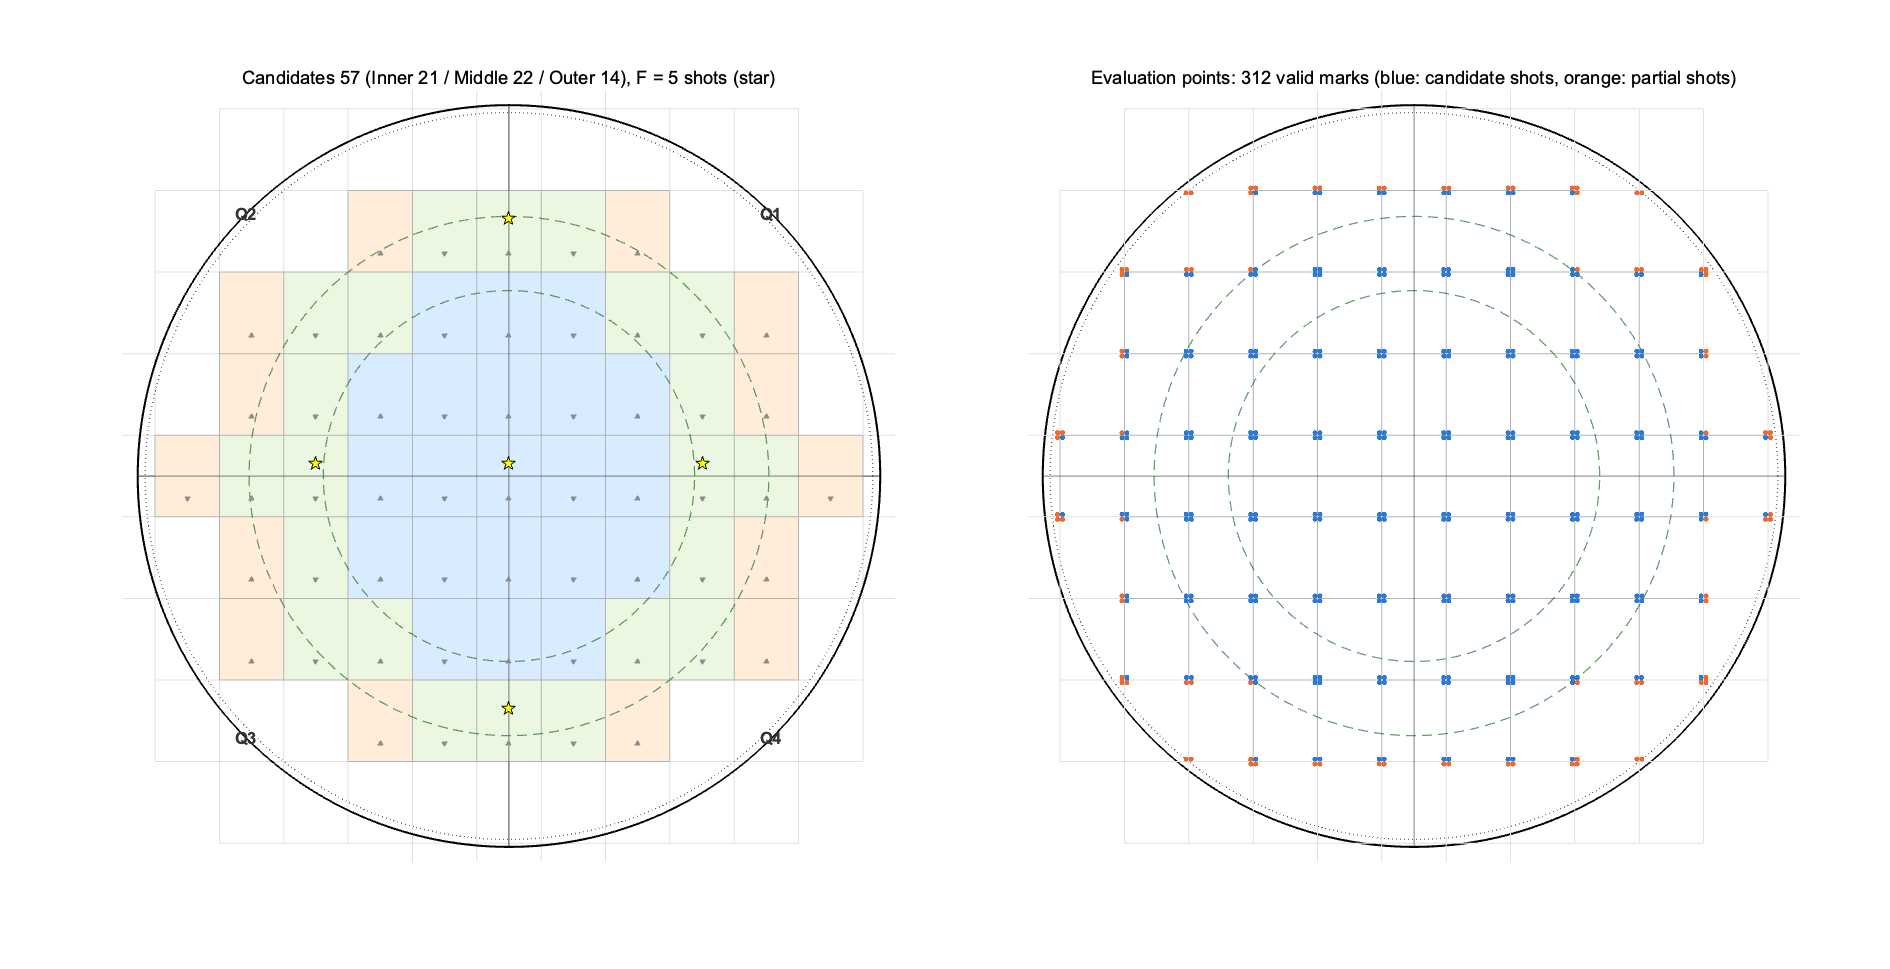
\includegraphics[width=\figw]{fig01_layout_overview.png}
  \caption{shot配置．左：候補shot（色は半径領域，☆は強制計測shot，▲▼はscan方向），右：残差の評価点（青：候補shotのmark，橙：partial shotのmark）．}
  \label{fig:layout}
\end{figure}

\subsection{比較sampling手法}

\begin{description}
  \item[Random] 制約なしで候補から一様に抽選した．抽選ごとに結果が大きく変わるため，各条件で200回抽選し，1000 waferの平均RMSの中央値・平均・P95・最良・最悪をまとめた．waferごとの比較には，平均RMSが中央値になった抽選を代表として用いた．rank不足の抽選はやり直し，回数を記録した．
  \item[Poisson Disk] 候補shot中心に対する離散Poisson disk sampling（dart throwing\cite{bridson2007}）．乱数で決めた順に，選んだ点すべてから距離$d$以上なら採用し，採用数が$N$以上となる最大の$d$を二分探索で決めた．超過分は最近接距離の小さい点から外した．20個の乱数初期値のうち，点間の最小距離が最大の解を代表解とした（残差は見ていない）．
  \item[Human] 人の配置を模擬したルールベース設計．中心shotを含め，残りを正規化半径0.45と0.78の2つの円上に円周長に比例して配り，外側の円は45°から，内側の円は半ピッチずらして等角度に目標点を置き，最寄りの候補shotを選ぶ．最適化は使わない．実際の配置をCSVから読み込むこともできる．
  \item[D-opt / I-opt] 制約なしのD最適・I最適計画．
  \item[Constrained D-opt / I-opt] 本手法（象限・半径・scan方向のhard制約）．
\end{description}

強制計測shotありの条件では，Random・Poisson・Humanにも強制shotを含め（Random + F など），さらに制約なしの拡張計画（D/I-opt Aug.），素朴な方法（Constr. D/I-opt Naive），本手法の制約付き拡張計画（Constr. D/I-opt Augmentation）を比較した．

\subsection{計測shot数}

HOWA次数ごとに，$4N\ge p_m$を満たす最小の$N$から，制約なしD最適でfull rankの設計が得られる最小shot数$N_\text{min}$をアルゴリズムで確認した（表\ref{tab:nmin}）．
計測shot数は$N_\text{min}$から$\lfloor 57/3\rfloor=19$まで1 shot刻みですべて評価した（adaptive gridは使っていない）．
強制計測shotありの条件は，強制shot数（5）より多い6 shotから評価した．

\begin{table}[htbp]
  \centering
  \caption{HOWA次数ごとの項数と最小shot数}
  \label{tab:nmin}
  \begin{tabular}{cccccc}
    \toprule
    HOWA次数 & 項数 $p_m$ & $\lceil p_m/4\rceil$ & $N_\text{min}$ & 評価したshot数 & 点数 \\
    \midrule
    3 & 10 & 3 & 3 & 3〜19 & 17 \\
    4 & 15 & 4 & 4 & 4〜19 & 16 \\
    5 & 21 & 6 & 6 & 6〜19 & 14 \\
    \bottomrule
  \end{tabular}
\end{table}

\subsection{mandatory shot条件}

強制計測shotは，中心shotと上下左右の十字（正規化半径0.52〜0.66）の5 shotとした（図\ref{fig:layout}の☆）．
このうち4 shotがMiddle領域に入り，scan方向はUp 3，Down 2である．
6 shotでは，Middle領域の上限（3）を強制shotだけで超えるため，制約付きの設計は存在しない（実行不能として記録）．

\subsection{実務制約条件}

主評価はhard制約（象限・半径・scan方向をすべて満たす交換だけを許す）で行った．
制約付き手法の全設計で制約違反が0であることを自動テストで確認した．

\subsection{HOWA 3〜5次条件}

各HOWA次数について，設計（D/I最適の目的関数）も補正（OLS）も同じ次数のモデルを使った．
Random・Poisson・Humanの配置は次数によらないが，Randomのrank判定は次数ごとに行った．

\subsection{Monte Carlo条件}

1000 waferを生成し，主評価条件（nominal：mark誤差0.5\,nm，scan方向依存成分1倍）に加え，mark誤差をlow／high，scan方向依存成分を0・0.5・2・4倍にした6条件を評価した．
各条件で同じ標準正規乱数を拡大縮小して使う（共通乱数）ため，条件間の比較も対応がある．

% ============================================================
\section{wafer面内傾向・計測データ生成}
% ============================================================

\subsection{Fringe Zernikeによる面内傾向}

真のwafer面内傾向は，補正モデル（HOWA多項式）とは別のFringe Zernike多項式で生成した．
これにより，補正モデルで表せない成分を含むmodel mismatchのある評価になる．
動径次数$n$・方位次数$m$の項のFringe番号は$j=(1+(n+|m|)/2)^2-2|m|+[m<0]$で，Z1〜Z36は一般的なFringe番号\cite{wyant1992}と一致する．
Zernikeは非正規化（端で最大1）とし，$\rho=r/R$，$\theta=\mathrm{atan2}(y,x)$で評価した．

\subsection{7次までの項から10〜20項をランダム選択}

「7次まで」を動径次数$n\le7$と解釈し，36項（Fringe番号Z1〜Z24，Z26〜Z31，Z37〜Z40，Z50，Z51）を候補とした．
waferごと・X/Yごとに項数を10〜20から一様に選び，その数の項を36項から重複なく選んだ．
$n\ge6$の項はHOWA 5次でも表せないため，すべての次数でmodel mismatchが残る．
（「Fringe番号の群$(n+|m|)/2\le7$」と解釈する設定も用意した．）

\subsection{Zernike係数の乱数生成}

係数は$a_k\sim N(0,\sigma_k^2)$，$\sigma_k=\sigma_0/\max(n_k,1)^\alpha$（$\sigma_0=3\nm$，$\alpha=1$）とし，高次の項ほど小さくした．
生成後のRMS（評価点312点）が1\,nmより小さいwaferは1\,nmへ，8\,nmより大きいwaferは8\,nmへ拡大縮小した．
1000 waferのX成分RMSの中央値は1.75\,nm，5〜95\%点は1.00〜5.05\,nmで，拡大縮小はX 220枚・Y 234枚に適用された（ほとんどが1\,nmへの拡大）．
分布・$\sigma_0$・$\alpha$・正規化の方法は設定で変えられ，乱数seedは結果に保存した．

\subsection{1000 wafer生成}

X成分$Z_x(u,v)$とY成分$Z_y(u,v)$は独立に生成した（同じ項を選び係数に相関を持たせる設定も用意した）．
1000 waferの真値・scan成分・mark誤差は一度だけ生成し，全手法で共有した．
全手法で同じwafer realizationを使ったことは，評価に使ったデータの指紋（重み付き総和）が全設計で一致することで確認した．

\subsection{scan方向依存成分}

shot $i$のscan方向を$s_i=+1$（Up），$-1$（Down）として，計測される値に次の成分を加えた．
\begin{description}
  \item[Model A] Up/Downで符号が反転するsystematic offset：$\eta_A=s_i\,a_w$，$a_w=0.3\nm\times(1+0.2\,\xi_w)$（$\xi_w\sim N(0,1)$，waferごと）．
  \item[Model B] Up/Downで符号が反転する低次の空間成分：$\eta_B=s_i(b_{1,w}u+b_{2,w}v)$，$b_{k,w}\sim N(0,0.5^2)$\,nm．
  \item[Model C] scan方向ごとに標準偏差が異なるshot単位の乱数：$\eta_C\sim N(0,\sigma_d^2)$，$\sigma_\text{Up}=0.15\nm$，$\sigma_\text{Down}=0.25\nm$（同じshotの4 markは同じ値）．
\end{description}
主評価（nominal）はA+B+Cの1倍で，評価点でのRMSは平均でA 0.30，B 0.30，C 0.21\,nm（X成分）である．
頑健性の評価では全体を0・0.5・2・4倍にした．
Model A・Bは，Up/Downの計測数が偏ると補正値に偏りとして写り込むので，scan方向制約の効果を調べる成分である．

\subsection{4 alignment markでの真値}

真値は全評価点（312 mark）で計算し，候補shotの228 markはその一部として使う．
markの座標はshot中心＋mark相対位置で，正規化半径$\rho\le0.98$の範囲にある．

\subsection{mark measurement noise}

mark計測誤差は各mark・X/Yで独立な$\epsilon\sim N(0,\sigma_\text{mark}^2)$とした．
計測値は
\begin{equation}
  z_x^\text{meas}=Z_x^\text{true}+\eta_x^\text{scan}+\epsilon_x,\qquad
  z_y^\text{meas}=Z_y^\text{true}+\eta_y^\text{scan}+\epsilon_y
\end{equation}
である．相関のある誤差は，標準正規乱数を作る部分を差し替えれば追加できる構造にした．

% ============================================================
\section{HOWA型高次補正シミュレーション}
% ============================================================

\subsection{HOWA 3次}

10項（$1,u,v,\dots,v^3$）．$N_\text{min}=3$（12 mark）．

\subsection{HOWA 4次}

15項．$N_\text{min}=4$（16 mark）．

\subsection{HOWA 5次}

21項．$\lceil21/4\rceil=6$で，$N_\text{min}=6$（24 mark）．

\subsection{OLS係数推定}

選んだshotの全markの計測値で，X・Yそれぞれ$\hat{\bm{a}}=\argmin\|\bm{z}-\bm{X}_S\bm{a}\|^2$を，正規方程式ではなくQR分解（$\bm{X}_S=\bm{Q}\bm{R}$，$\hat{\bm{a}}=\bm{R}^{-1}\bm{Q}^\top\bm{z}$）で求めた．
1000 wafer分は右辺を並べて一度に解いた．
誤差のない多項式データから係数を$10^{-6}$以内で復元できること，評価した全設計で係数が有限で，$\bm{R}$の対角成分の比が$10^{8}$未満であることを自動テストで確認した．

\subsection{wafer全面への補正}

推定した係数で，全shot（partial shotを含む）のusable領域内の全mark 312点に補正を展開した．
partial shotの領域は候補shotの外側にあり，補正は外挿になる．

\subsection{補正後残差}

残差は，計測誤差とscan成分を含まない真の面内傾向に対して
\begin{equation}
  e_x=Z_x^\text{true}-\bm{f}^\top\hat{\bm{a}}^{(x)},\qquad e_y=Z_y^\text{true}-\bm{f}^\top\hat{\bm{a}}^{(y)}
\end{equation}
とした．これにより，sampling配置と誤差による推定誤差（バイアスと分散）を評価する．
真値にscan成分を含める設定も用意した．

% ============================================================
\section{評価指標}
% ============================================================

\subsection{Residual RMS}

waferごとに，評価点$E'$（312点）で$\mathrm{RMS}_x=\sqrt{\overline{e_x^2}}$，$\mathrm{RMS}_y=\sqrt{\overline{e_y^2}}$，$\mathrm{RMS}_\text{vec}=\sqrt{\overline{e_x^2+e_y^2}}$を求めた．
最重要指標は$\mathrm{RMS}_\text{vec}$で，以下「RMS」と書く．候補shotのmark（228点）だけで求めた値（interior RMS）も出力した．

\subsection{P95 / P99 / Max residual}

waferごとの残差の大きさ$|\bm{e}|=\sqrt{e_x^2+e_y^2}$の95\%点・99\%点・最大値を求めた．
百分位点はすべて線形補間（Excel の PERCENTILE.INC と同じ定義）で計算した．
1000 waferについて，各指標の平均・中央値・標準偏差・P90・P95・P99・最悪値をまとめた．

\subsection{D-efficiency}

同じ次数・同じshot数の制約なしD最適設計$S_D^*$を基準に，$D_\text{eff}(S)=\left(\det\bm{M}(S)/\det\bm{M}(S_D^*)\right)^{1/p}$とした．

\subsection{I-efficiency}

同じ次数・同じshot数の制約なしI最適設計$S_I^*$を基準に，$I_\text{eff}(S)=I(S_I^*)/I(S)$とした．
交換法は発見的なので，制約付き設計などで1をわずかに超えることがありうる．

\subsection{quadrant coverage}

$B_Q=\max_q N_q-\min_q N_q$．

\subsection{radial coverage}

$B_R=\max_r N_r-\min_r N_r$（Inner・Middle・Outerの3領域）．

\subsection{scan-direction balance}

$B_S=|N_\text{up}-N_\text{down}|$．

\subsection{constraint violation}

象限・半径・scan方向の上下限からのはみ出しshot数（式(\ref{eq:bounds})の上下限に対する$\max(0,L-N)+\max(0,N-U)$の合計）と，含まれていない強制計測shot数を設計ごとに数えた．
制約のない手法にも同じ上下限を当てはめて集計した．

\subsection{必要shot数削減効果}

基準手法（主にHuman）のshot数$N_\text{ref}$での平均RMS（またはwaferごとのRMSのP95）を目標とし，各手法がその目標以下になる最小shot数$N^*$を求め，$\text{Measurement reduction}=(N_\text{ref}-N^*)/N_\text{ref}\times100\,\%$とした．

\subsection{optimization calculation time}

設計1件（multi-start全体）の計算時間を記録した．計算環境はMATLAB R2022b（Apple Silicon上のRosetta 2，並列化なし）である．

\subsection*{統計的な比較}

提案法と比較法の差は，同じwaferでの差$\Delta\mathrm{RMS}_w=\mathrm{RMS}_{\text{比較},w}-\mathrm{RMS}_{\text{提案},w}$と改善率$100\,\Delta\mathrm{RMS}_w/\mathrm{RMS}_{\text{比較},w}$で評価した．
平均の$t$信頼区間に加え，waferを復元抽出するbootstrap（2000回，百分位法）\cite{efron1993}で平均・中央値・平均改善率の95\%信頼区間を求め，提案法が勝ったwaferの割合（勝率）も示した．
平均値だけで優劣を判断せず，信頼区間が0をまたがないことを「差がある」の目安とした．

% ============================================================
\section{評価結果}
\label{sec:results}
% ============================================================

以下，特に断らない限り主評価条件（mark誤差0.5\,nm，scan方向依存成分1倍）・強制計測shotなしの結果である．
表中の手法名は，C-D-opt＝Constrained D-opt，C-I-opt＝Constrained I-optの略である．
「改善率」は$(\mathrm{RMS}_\text{比較}-\mathrm{RMS}_\text{提案})/\mathrm{RMS}_\text{比較}\times100$で，正なら提案法（制約付き）の残差が小さい．

\subsection{sampling map比較}

図\ref{fig:map}にHOWA 4次・$N=12$のsampling mapを示す．
制約なしのD-opt・I-optは，候補の最外周（Outer）とwafer中心にshotを集め，Middle領域をほとんど選ばない．
HOWA 5次では，D-optは$N\le13$でMiddleを1つも選ばず，$N\ge11$ではOuterの候補14 shotのうち10 shotを選んだ．
その結果，半径領域の上下限をほぼすべてのshot数で外れ（$B_R$は最大10），scan方向もUp/Downの差$B_S$が最大10（I-optは12）に偏った．
制約付き設計（C-D-opt・C-I-opt）は，外周を優先しつつInner・Middleにも配分し，Up/Downを同数（奇数では差1）にそろえた．
Poisson・Humanは見た目は均等だが，scan方向を考慮しないため，列ごとにUp/Downが交互になるshot配置との組合せでUp/Downが偏ることが多かった．
HOWA 4次・$N=12$では，C-D-optとC-I-optが同じ設計になった．

\begin{figure}[htbp]
  \centering
  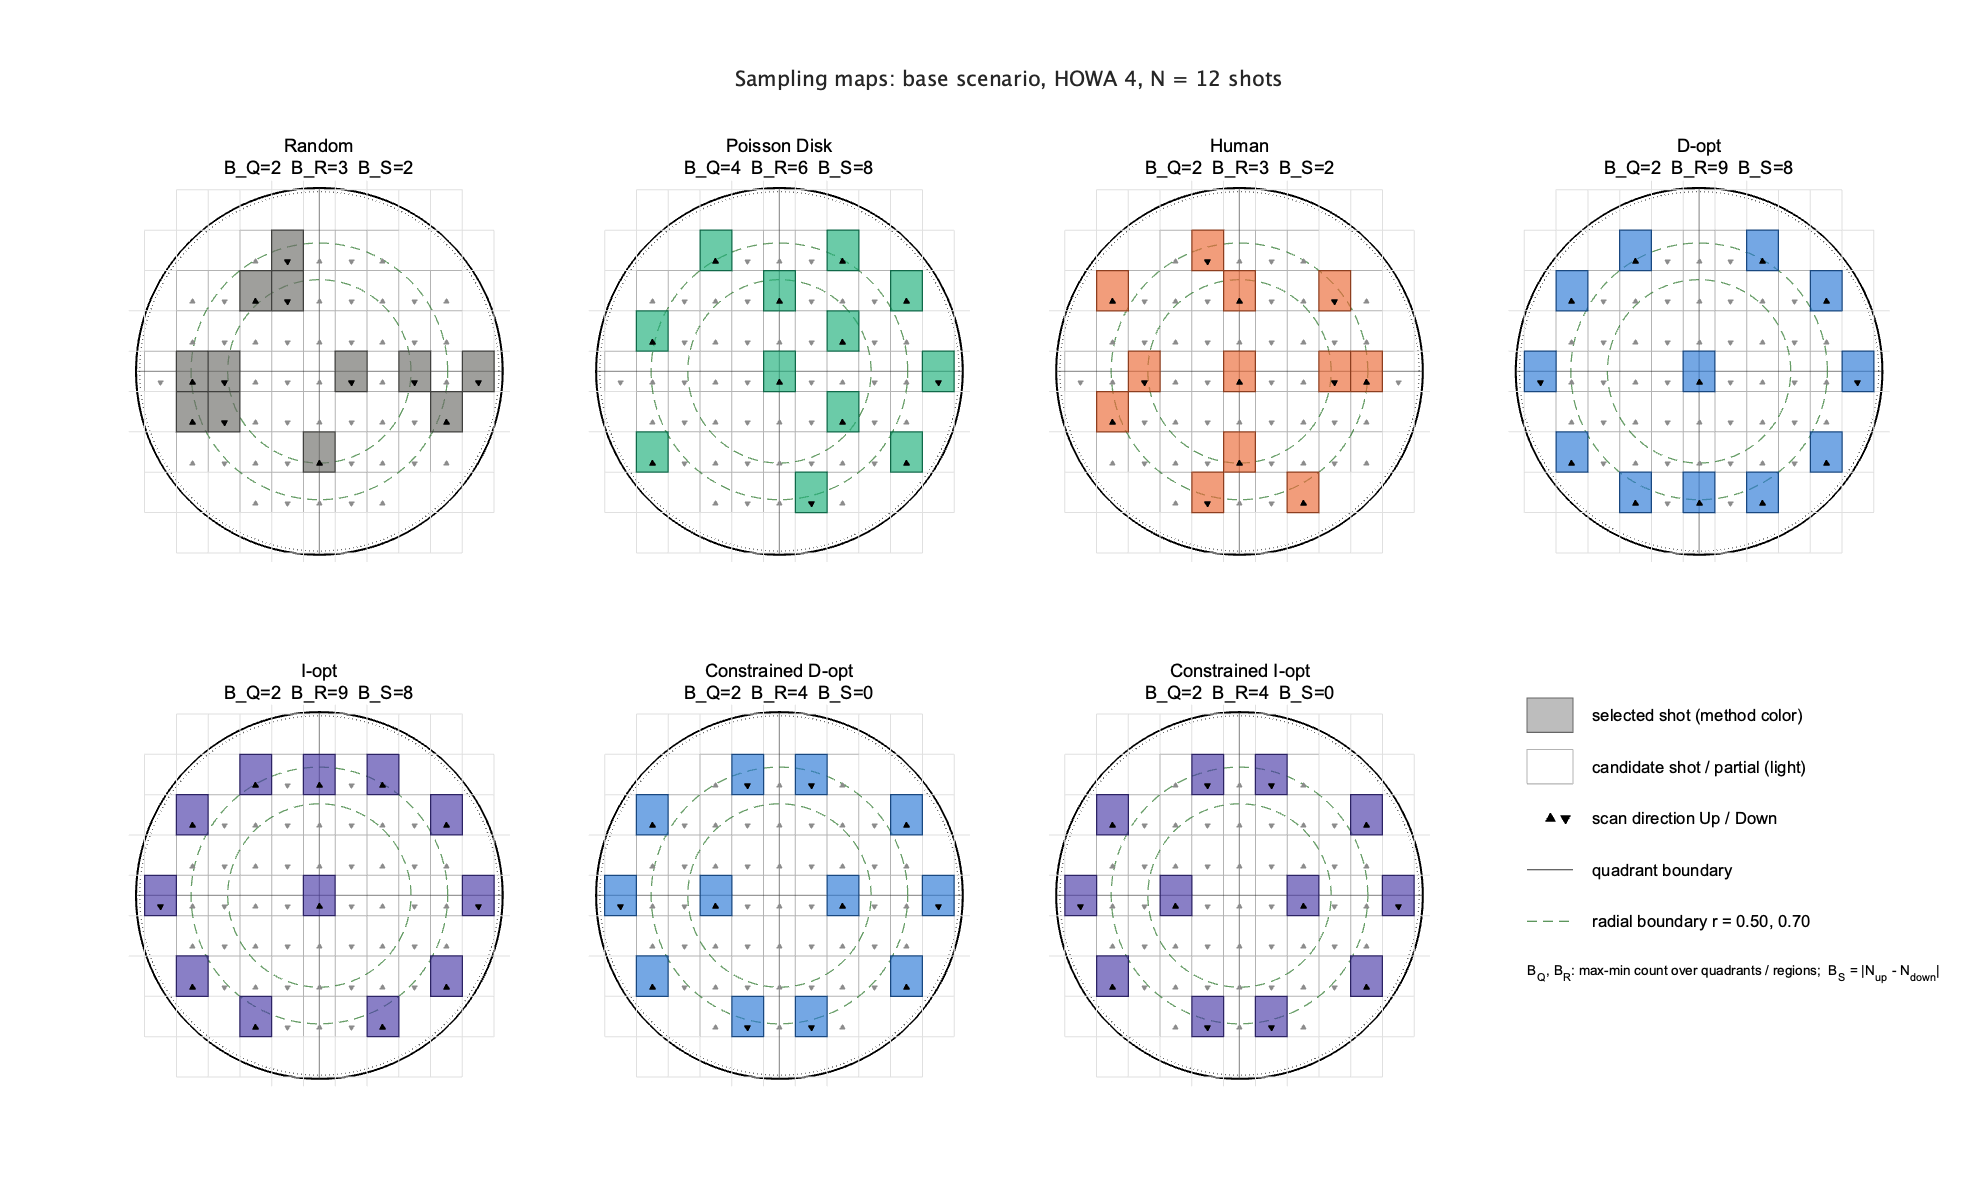
\includegraphics[width=\figw]{fig02_sampling_map_base_howa4_N12.png}
  \caption{sampling map（HOWA 4次，$N=12$，強制計測shotなし）．塗りが選んだshot，▲▼はscan方向，実線は象限境界，緑の破線は半径領域境界．各図の$B_Q$・$B_R$・$B_S$はcoverage指標．}
  \label{fig:map}
\end{figure}

\subsection{D/I efficiency比較}

表\ref{tab:eff}と図\ref{fig:eff}に効率を示す．
制約付き設計のD-efficiencyは，評価した全shot数の中央値で3次0.94・4次0.91・5次0.88（C-D-opt）で，I-efficiencyは同じく0.92・0.83・0.72だった．
制約の代償は次数が高いほど，shot数が少ないほど大きい（5次・$N=8$でD 0.86，I 0.62）．
一方，Human（D 0.44〜0.63）・Poisson（0.60〜0.81）・Random（抽選の中央値0.12〜0.56）よりは大幅に高い．
なお，$N\ge8$では制約なしのD-optのI-efficiencyは0.84以上，I-optのD-efficiencyは0.95以上で，この問題ではD最適とI最適の設計はよく似ていた（$N_\text{min}$付近ではそれぞれ0.52・0.70まで下がる）．

\begin{table}[htbp]
  \centering
  \caption{D/I-efficiency（同じ次数・同じshot数の制約なしD-opt / I-optを1とする．Randomは200抽選の中央値）}
  \label{tab:eff}
  \small
\begin{tabular}{clrrrrrr}
\toprule
次数 & 手法 & \multicolumn{2}{c}{$N=8$} & \multicolumn{2}{c}{$N=12$} & \multicolumn{2}{c}{$N=19$} \\
 & & D & I & D & I & D & I \\
\midrule
\multirow{7}{*}{3} & Random & 0.31 & 0.07 & 0.41 & 0.17 & 0.56 & 0.34 \\
 & Poisson & 0.73 & 0.62 & 0.81 & 0.77 & 0.72 & 0.59 \\
 & Human & 0.59 & 0.42 & 0.62 & 0.58 & 0.63 & 0.55 \\
 & D-opt & 1.00 & 0.85 & 1.00 & 1.00 & 1.00 & 0.99 \\
 & I-opt & 0.98 & 1.00 & 0.99 & 1.00 & 1.00 & 1.00 \\
 & C-D-opt & 0.91 & 0.84 & 0.95 & 0.94 & 0.97 & 0.95 \\
 & C-I-opt & 0.91 & 0.88 & 0.92 & 0.94 & 0.97 & 0.96 \\
\midrule
\multirow{7}{*}{4} & Random & 0.22 & 0.01 & 0.31 & 0.06 & 0.47 & 0.20 \\
 & Poisson & 0.67 & 0.50 & 0.74 & 0.58 & 0.66 & 0.44 \\
 & Human & 0.52 & 0.32 & 0.52 & 0.38 & 0.56 & 0.44 \\
 & D-opt & 1.00 & 0.99 & 1.00 & 1.00 & 1.00 & 0.99 \\
 & I-opt & 0.98 & 1.00 & 1.00 & 1.00 & 1.00 & 1.00 \\
 & C-D-opt & 0.88 & 0.79 & 0.91 & 0.85 & 0.96 & 0.92 \\
 & C-I-opt & 0.88 & 0.83 & 0.91 & 0.85 & 0.96 & 0.94 \\
\midrule
\multirow{7}{*}{5} & Random & 0.12 & 0.00 & 0.22 & 0.01 & 0.38 & 0.08 \\
 & Poisson & 0.62 & 0.32 & 0.69 & 0.49 & 0.60 & 0.30 \\
 & Human & 0.45 & 0.14 & 0.44 & 0.27 & 0.49 & 0.34 \\
 & D-opt & 1.00 & 0.94 & 1.00 & 0.99 & 1.00 & 0.99 \\
 & I-opt & 0.98 & 1.00 & 1.00 & 1.00 & 1.00 & 1.00 \\
 & C-D-opt & 0.86 & 0.62 & 0.89 & 0.62 & 0.96 & 0.87 \\
 & C-I-opt & 0.83 & 0.66 & 0.83 & 0.76 & 0.93 & 0.91 \\
\bottomrule
\end{tabular}
\end{table}

\begin{figure}[htbp]
  \centering
  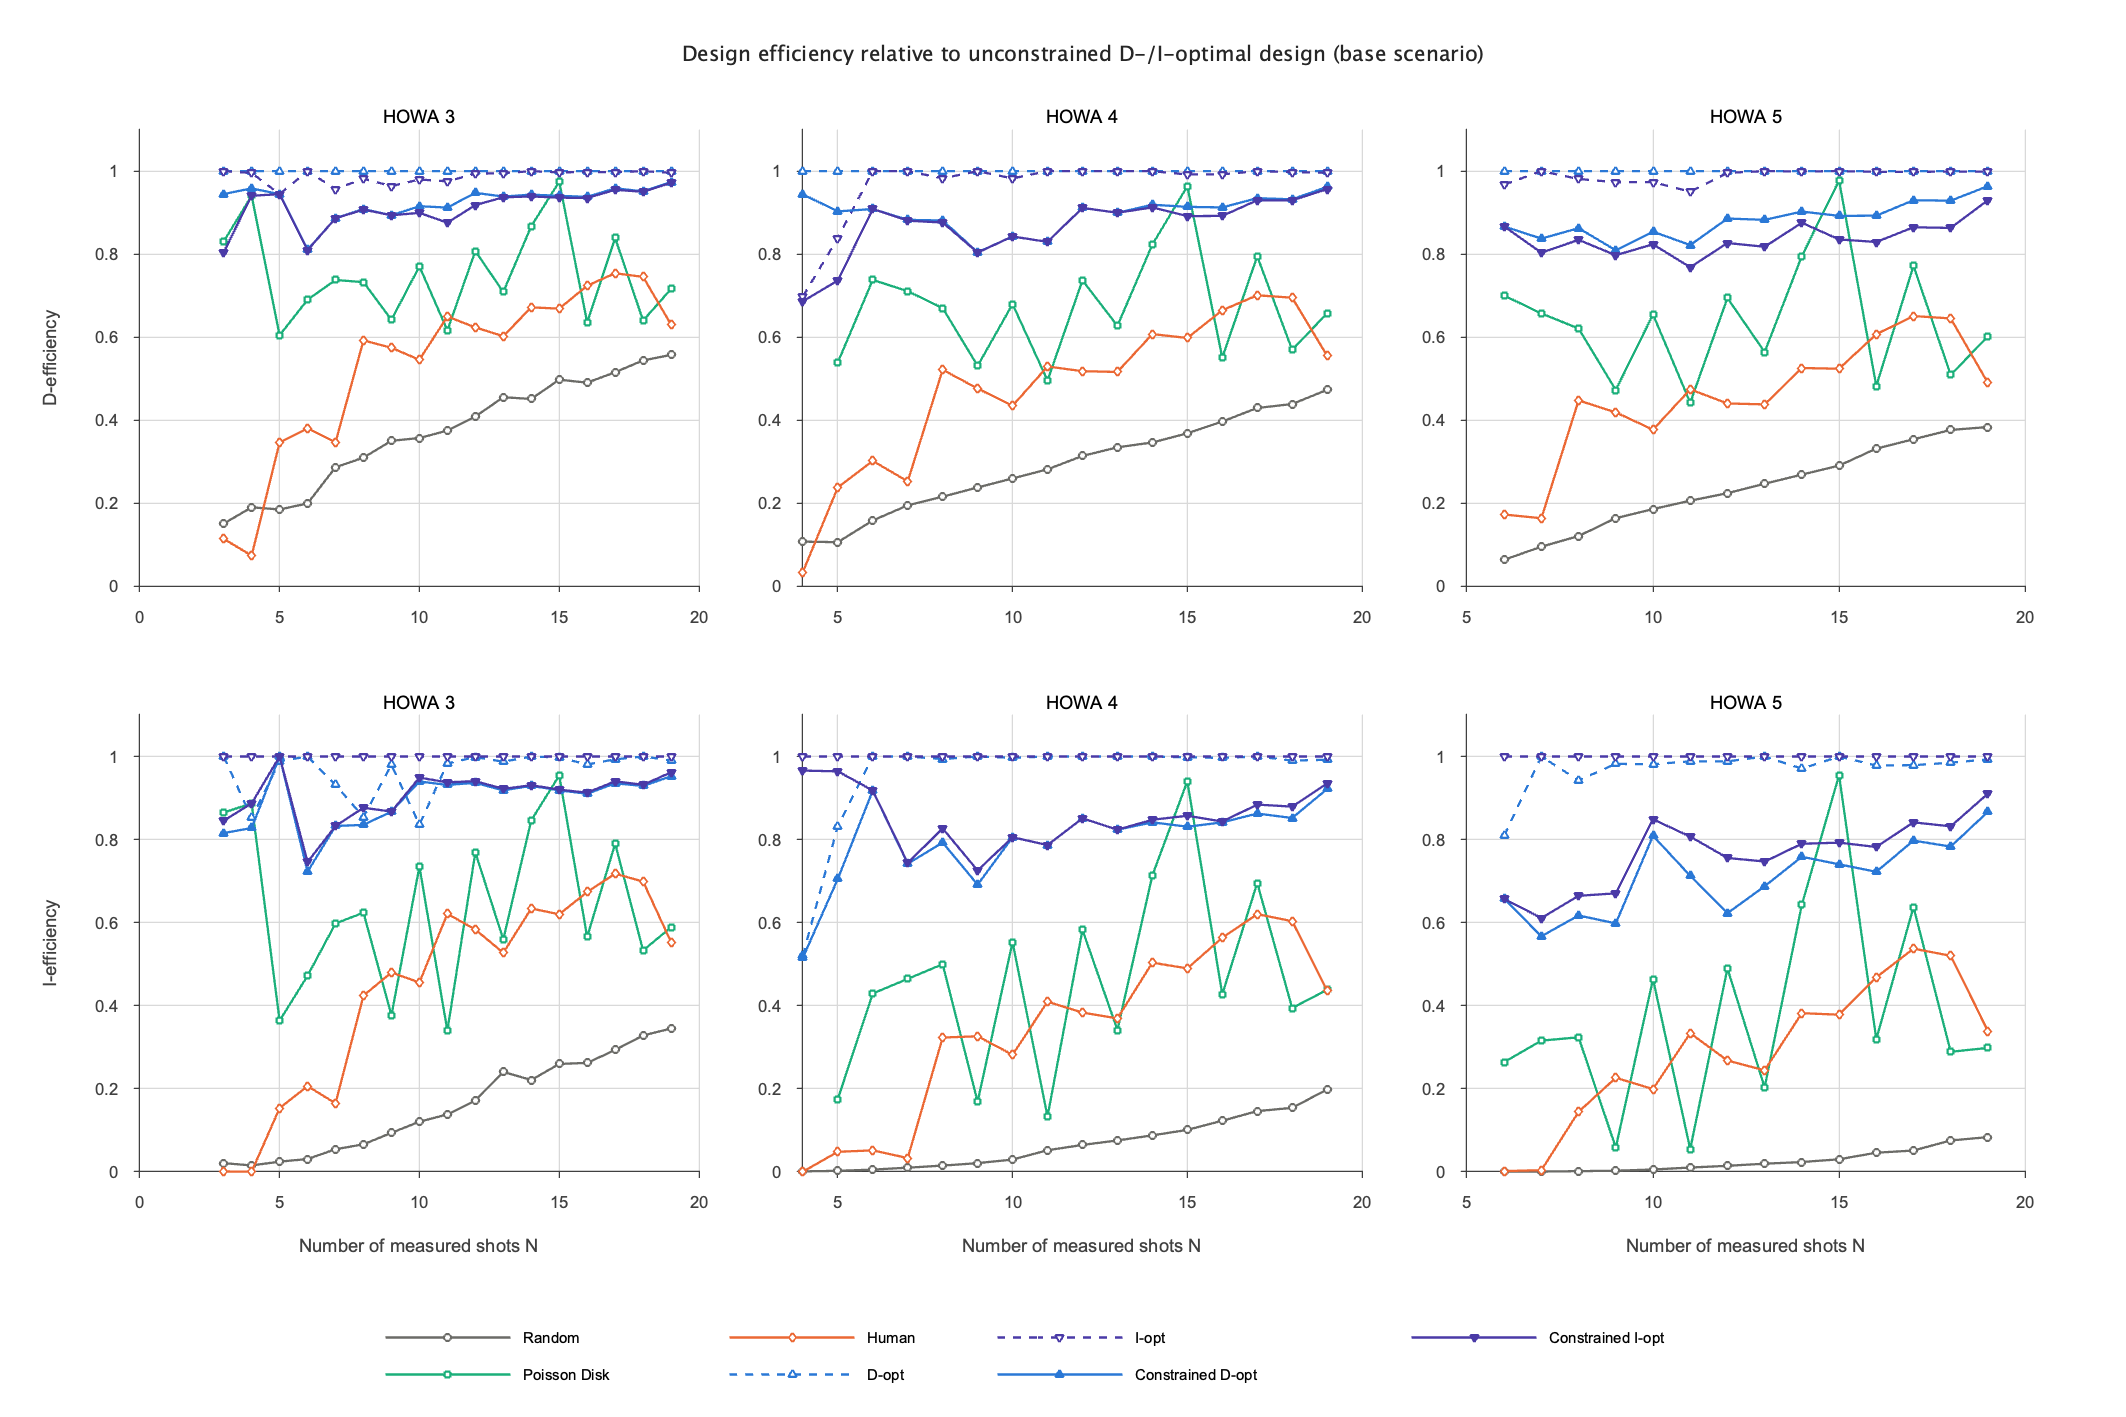
\includegraphics[width=\figw]{fig06_efficiency_base.png}
  \caption{計測shot数に対するD-efficiency（上）とI-efficiency（下）．}
  \label{fig:eff}
\end{figure}

\subsection{coverage比較}

表\ref{tab:violation}に，全次数・全shot数の設計（各手法47設計）での制約違反の割合とcoverage指標の平均を示す（図\ref{fig:coverage}はHOWA 4次の例）．
制約なしD-optは半径領域制約を100\%，scan方向制約を91\%の設計で外れた．
Human・Poissonは象限はほぼ満たすが，scan方向制約をそれぞれ64\%・77\%の設計で外れた．
Randomは85\%の抽選がいずれかの制約を外れた．
提案法（制約付き）は全設計で違反0であり，強制計測shotありの条件でも，制約付きの拡張計画・素朴な方法とも違反0，強制shotの欠落0だった（自動テストでも確認）．

\begin{table}[htbp]
  \centering
  \caption{制約違反の割合とcoverage指標（強制計測shotなし，全次数・全shot数）．Randomは抽選のうち違反したものの割合}
  \label{tab:violation}
  \small
\begin{tabular}{lrrrrrrr}
\toprule
手法 & 象限 & 半径 & scan & いずれか & $\bar{B}_Q$ & $\bar{B}_R$ & $\bar{B}_S$ \\
\midrule
Random（抽選の割合） & 41\% & 35\% & 62\% & 85\% & 3.07 & 3.27 & 2.47 \\
Poisson（設計の割合） & 19\% & 38\% & 77\% & 89\% & 2.04 & 3.74 & 3.70 \\
Human（設計の割合） & 0\% & 26\% & 64\% & 77\% & 1.45 & 2.79 & 3.32 \\
D-opt（設計の割合） & 0\% & 100\% & 91\% & 100\% & 1.64 & 7.62 & 5.11 \\
I-opt（設計の割合） & 0\% & 96\% & 89\% & 98\% & 1.49 & 7.28 & 5.40 \\
C-D-opt（設計の割合） & 0\% & 0\% & 0\% & 0\% & 1.55 & 3.38 & 0.51 \\
C-I-opt（設計の割合） & 0\% & 0\% & 0\% & 0\% & 1.60 & 3.32 & 0.51 \\
\bottomrule
\end{tabular}
\end{table}

\begin{figure}[htbp]
  \centering
  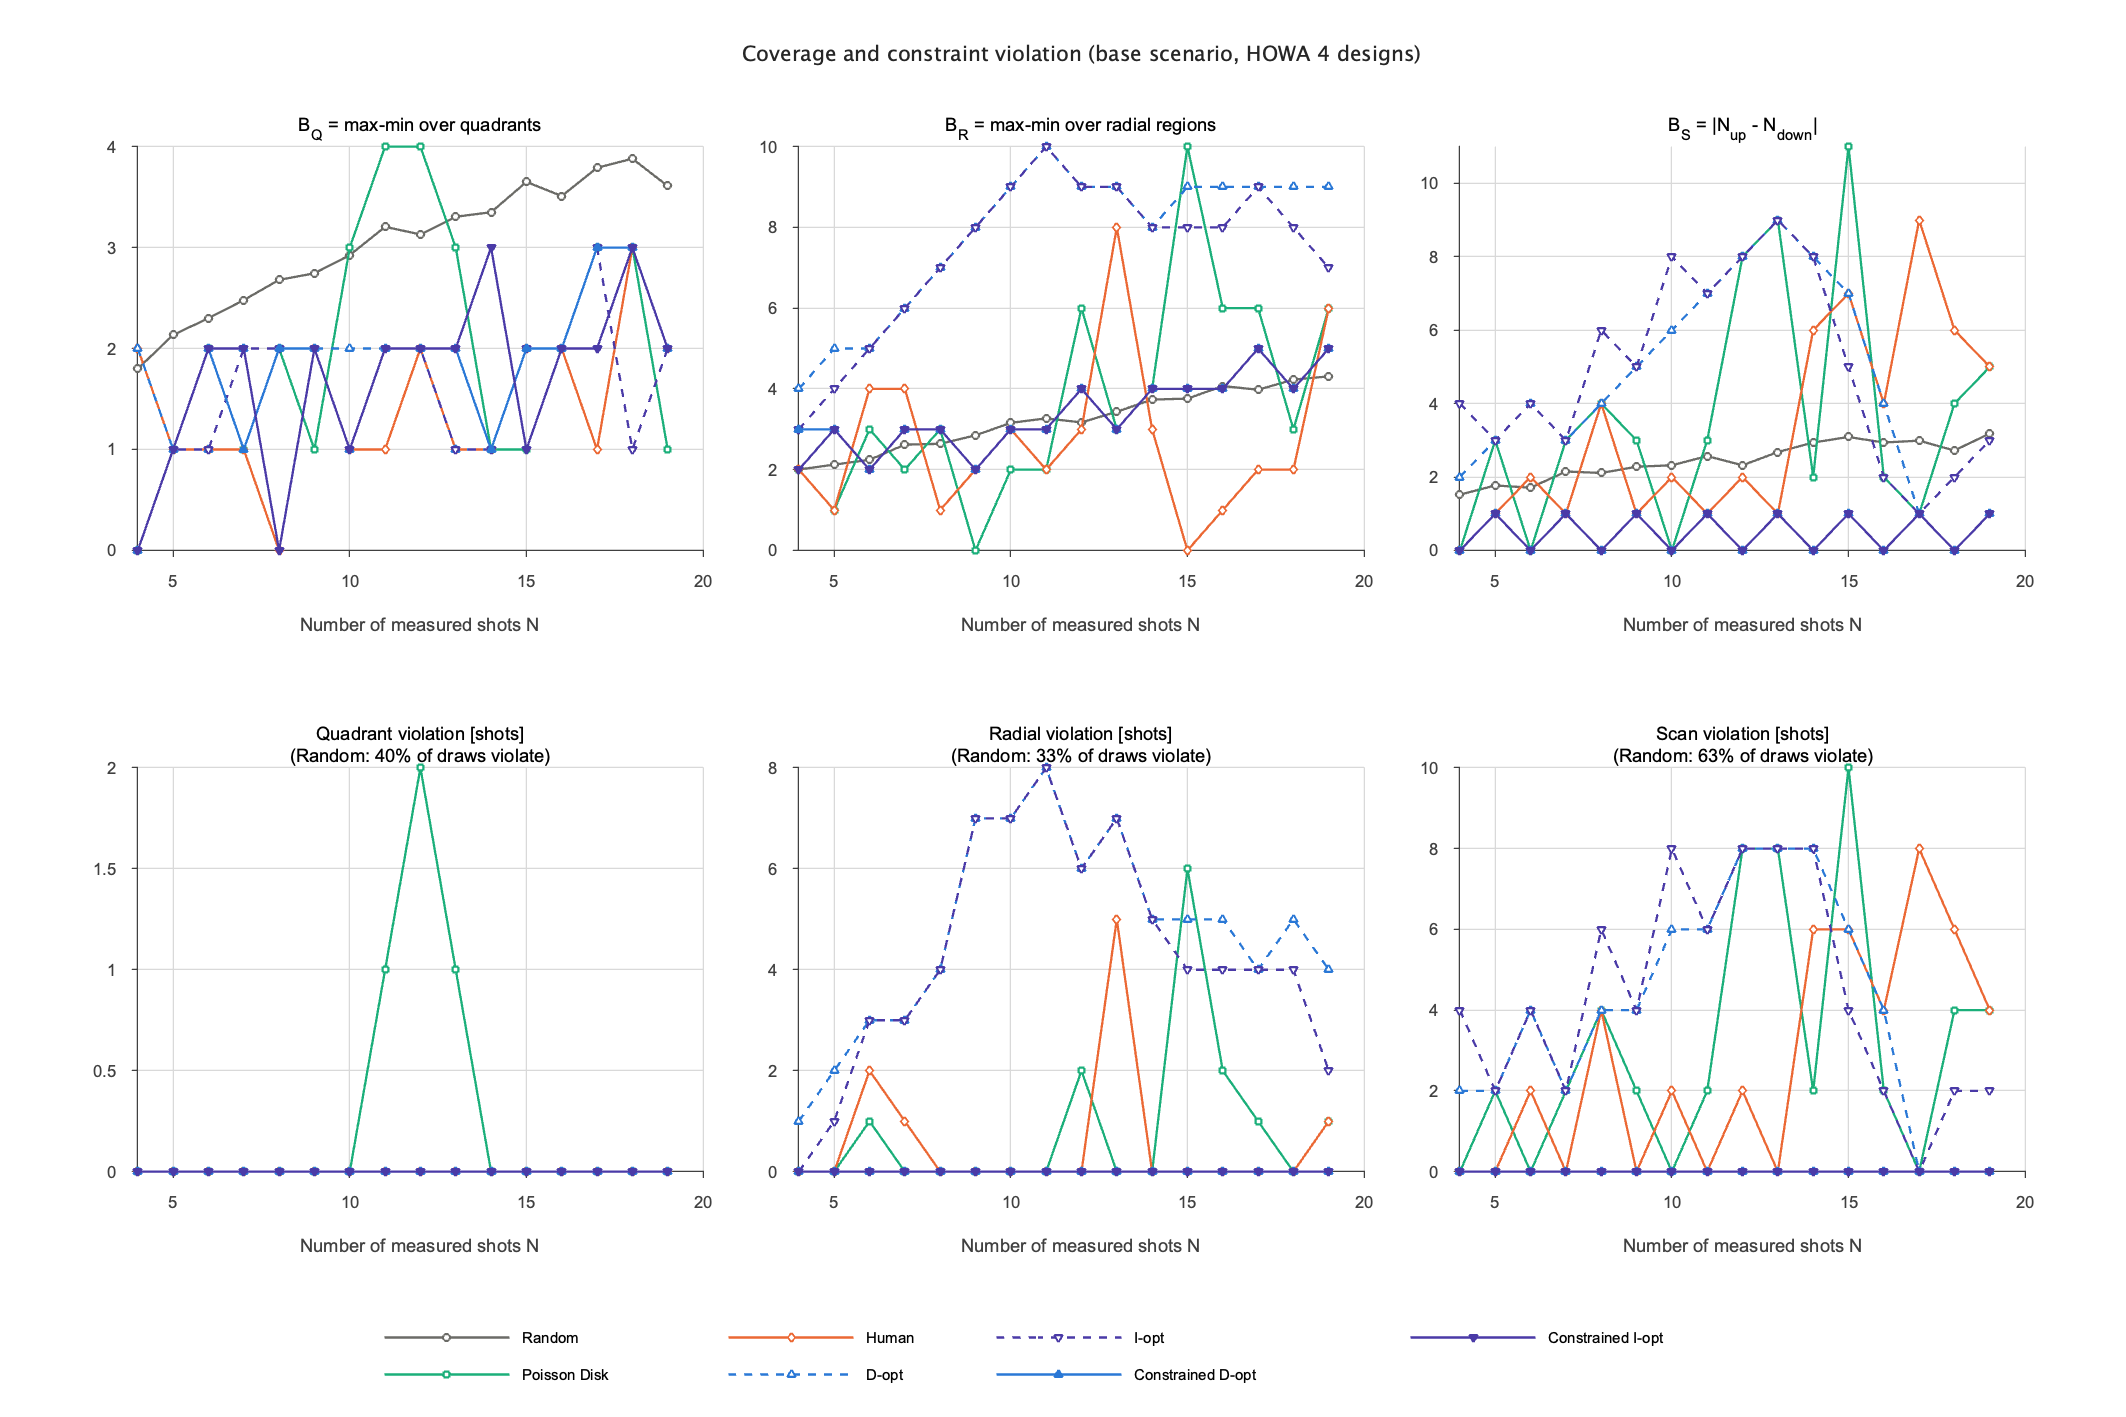
\includegraphics[width=\figw]{fig07_coverage_base.png}
  \caption{coverage指標（上）と制約違反（下，HOWA 4次の設計）．}
  \label{fig:coverage}
\end{figure}

\subsection{1000 waferのResidual RMS}

表\ref{tab:rms}に1000 waferの平均RMSを，図\ref{fig:rms}にshot数依存性を，図\ref{fig:dist}に$N=12$での分布を示す．
表の「下限」は，計測誤差もscan成分もなく全評価点を使ったときのHOWA補正残差（モデル不一致の下限）の平均である．

\begin{table}[htbp]
  \centering
  \caption{平均Residual RMS [nm]（1000 wafer，主評価条件，強制計測shotなし．太字は各行の最小）}
  \label{tab:rms}
  \small
\begin{tabular}{crrrrrrrrr}
\toprule
次数 & $N$ & Random & Poisson & Human & D-opt & I-opt & C-D-opt & C-I-opt & 下限 \\
\midrule
\multirow{6}{*}{3} & 6 & 4.87 & 1.60 & 1.98 & \textbf{1.34} & \textbf{1.34} & 1.40 & 1.40 & 0.77 \\
 & 8 & 2.96 & 1.42 & 1.47 & 1.31 & \textbf{1.22} & 1.30 & 1.30 &  \\
 & 10 & 2.29 & 1.28 & 1.44 & 1.23 & \textbf{1.16} & 1.20 & 1.21 &  \\
 & 12 & 1.90 & 1.19 & 1.36 & 1.09 & 1.06 & \textbf{1.01} & 1.05 &  \\
 & 15 & 1.57 & 1.05 & 1.24 & 0.97 & 0.99 & \textbf{0.96} & 0.98 &  \\
 & 19 & 1.41 & 1.20 & 1.24 & 0.94 & \textbf{0.94} & 0.94 & 0.95 &  \\
\midrule
\multirow{6}{*}{4} & 6 & 14.02 & 2.06 & 4.15 & \textbf{1.43} & \textbf{1.43} & 1.54 & 1.54 & 0.55 \\
 & 8 & 6.28 & 1.55 & 1.67 & \textbf{1.18} & 1.20 & 1.26 & 1.27 &  \\
 & 10 & 4.10 & 1.32 & 1.63 & \textbf{1.10} & 1.13 & 1.15 & 1.15 &  \\
 & 12 & 2.73 & 1.16 & 1.55 & 0.99 & 0.99 & \textbf{0.97} & \textbf{0.97} &  \\
 & 15 & 2.10 & 0.95 & 1.30 & 0.93 & \textbf{0.90} & 0.94 & 0.97 &  \\
 & 19 & 1.60 & 1.20 & 1.35 & 0.86 & \textbf{0.86} & 0.89 & 0.87 &  \\
\midrule
\multirow{6}{*}{5} & 6 & 539 & 5.05 & 37.68 & 2.91 & \textbf{2.54} & 3.68 & 3.76 & 0.39 \\
 & 8 & 28.53 & 2.32 & 3.31 & \textbf{1.38} & 1.39 & 1.56 & 1.56 &  \\
 & 10 & 10.75 & 1.65 & 2.30 & \textbf{1.13} & 1.17 & 1.26 & 1.32 &  \\
 & 12 & 5.56 & 1.29 & 1.94 & 0.95 & \textbf{0.93} & 1.03 & 1.08 &  \\
 & 15 & 3.69 & 0.92 & 1.54 & \textbf{0.91} & \textbf{0.91} & 0.95 & 1.06 &  \\
 & 19 & 2.43 & 1.43 & 1.65 & \textbf{0.88} & 0.88 & 0.90 & 0.93 &  \\
\bottomrule
\end{tabular}
\end{table}

\begin{figure}[htbp]
  \centering
  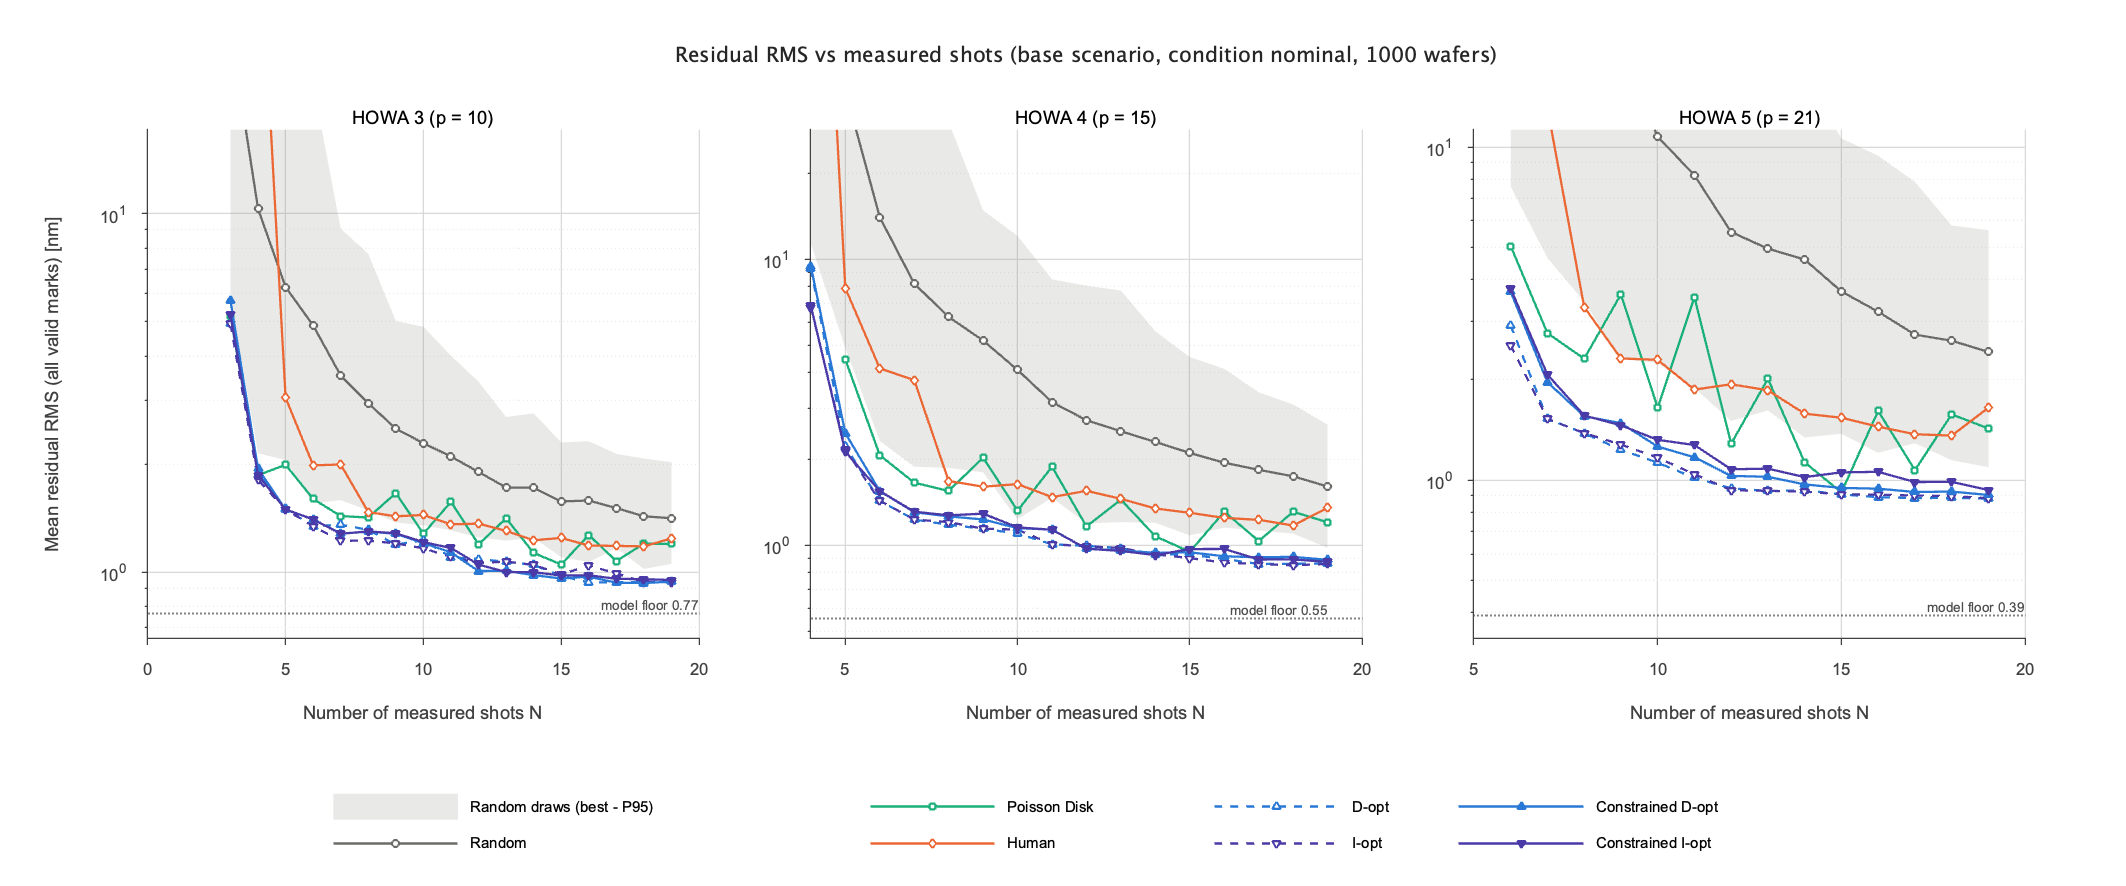
\includegraphics[width=\figw]{fig03_rms_vs_shots_base.png}
  \caption{計測shot数に対する平均Residual RMS（全評価点）．灰色の帯はRandom 200抽選の平均RMSの最良〜P95，点線はモデル不一致の下限．}
  \label{fig:rms}
\end{figure}

\begin{figure}[htbp]
  \centering
  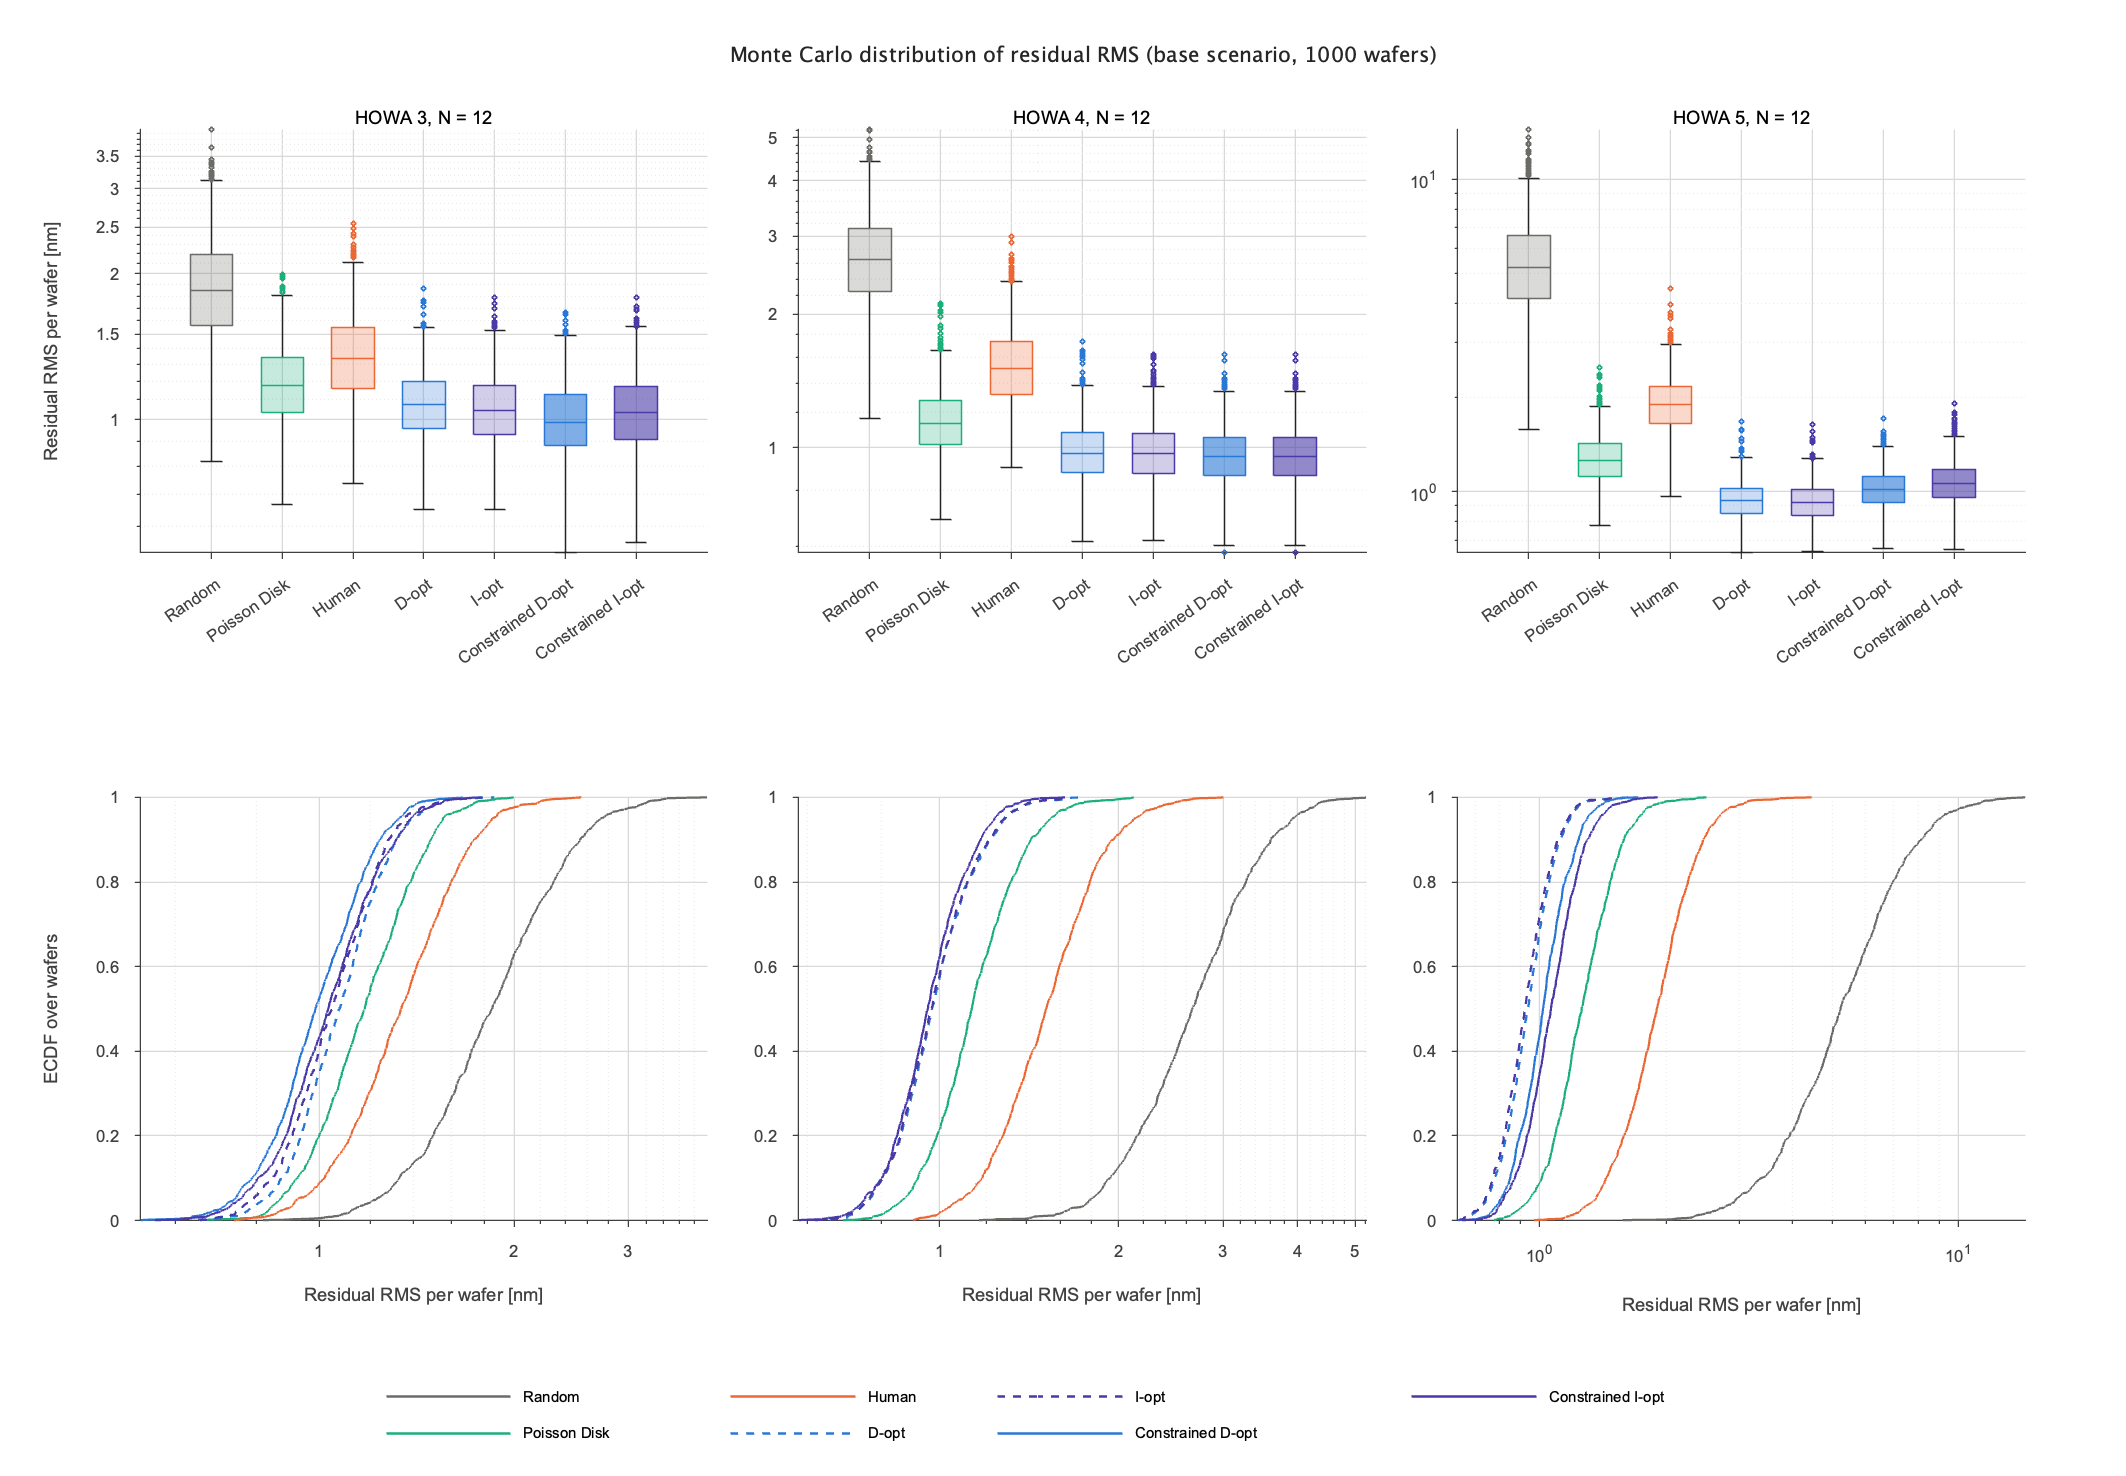
\includegraphics[width=\figw]{fig05_distribution_base_N12.png}
  \caption{$N=12$での1000 waferのRMSの分布（上：箱ひげ図，下：経験分布関数）．}
  \label{fig:dist}
\end{figure}

主な結果は次のとおりである．

\begin{enumerate}
  \item \textbf{Random・Human・Poissonに対しては，制約付き設計が大きく小さい残差を与えた．}
    $N=8$〜19の12点について，平均RMSどうしの改善率の中央値は，C-D-optでHumanに対し3次20.5\%・4次26.9\%・5次38.6\%，Poissonに対し18.6\%・22.3\%・34.8\%，Random（代表抽選）に対し42\%・60\%・79\%だった．
    waferを復元抽出したbootstrap 95\%信頼区間は，Human・Randomに対しては全shot数で0を上回り，Poissonに対しては12点中11〜12点で0を上回った．
  \item \textbf{制約なしのD/I最適に対しては，次数によって結果が分かれた．}
    3次では同等（C-D-optのD-optに対する改善率の中央値+0.9\%，12点中8点で有意に良く3点で有意に悪い），4次では$-3.8\%$（10点で有意に悪い），5次では$-7.5\%$（12点すべてで有意に悪い）だった．
    C-I-optは5次で$-15.3\%$とさらに差が大きかった．
    つまり，実務制約を満たすことの代償は残差で数\%〜十数\%であり，次数が高いほど大きい．
  \item \textbf{$N_\text{min}$付近では全手法の残差が大きい．}
    5次の$N=6$（24 markで21項）ではD-optでも2.91\,nmで，$N=8$の1.38\,nmの2倍以上だった．Randomの代表抽選は539\,nm，Humanは37.7\,nmと推定が破綻に近い．
  \item \textbf{分布全体でも順位は変わらない．}
    図\ref{fig:dist}の経験分布関数は，制約付き・制約なしのD/I最適がほぼ重なり，Poisson・Human・Randomが右（残差が大きい側）にずれる形で，平均値の比較と同じ順位だった．
\end{enumerate}

$N=12$でのpaired comparisonを表\ref{tab:paired}に示す．
4次では制約付き設計がD-optより1.5\%（95\%CI 0.9〜2.2\%）小さく，3次では7.3\%小さかったが，5次では9.6\%大きかった．
勝率（提案法の方が残差の小さいwaferの割合）は，Human・Randomに対して0.96〜1.00だった．

\begin{table}[htbp]
  \centering
  \caption{$N=12$でのpaired comparison（1000 wafer）．$\Delta$RMSと改善率は正なら提案法が良い．CIはbootstrap（2000回）の95\%信頼区間}
  \label{tab:paired}
  \small
\begin{tabular}{cclrrrr}
\toprule
次数 & 提案法 & 比較法 & 平均$\Delta$RMS [nm] & 平均改善率 [\%] & 95\%CI [\%] & 勝率 \\
\midrule
\multirow{10}{*}{3} & C-D-opt & Random & +0.895 & +45.1 & [+44.4, +45.8] & 1.00 \\
 & C-D-opt & Poisson & +0.188 & +15.2 & [+14.7, +15.7] & 0.95 \\
 & C-D-opt & Human & +0.358 & +25.1 & [+24.4, +25.7] & 0.98 \\
 & C-D-opt & D-opt & +0.081 & +7.3 & [+6.9, +7.9] & 0.82 \\
 & C-D-opt & I-opt & +0.053 & +4.8 & [+4.3, +5.3] & 0.74 \\
 & C-I-opt & Random & +0.853 & +42.8 & [+42.0, +43.5] & 0.99 \\
 & C-I-opt & Poisson & +0.145 & +11.5 & [+10.9, +12.2] & 0.87 \\
 & C-I-opt & Human & +0.316 & +22.0 & [+21.3, +22.7] & 0.96 \\
 & C-I-opt & D-opt & +0.038 & +3.4 & [+2.8, +4.0] & 0.67 \\
 & C-I-opt & I-opt & +0.010 & +0.8 & [+0.2, +1.4] & 0.56 \\
\midrule
\multirow{10}{*}{4} & C-D-opt & Random & +1.762 & +62.8 & [+62.3, +63.4] & 1.00 \\
 & C-D-opt & Poisson & +0.190 & +15.4 & [+14.7, +16.0] & 0.92 \\
 & C-D-opt & Human & +0.577 & +35.6 & [+35.0, +36.4] & 0.99 \\
 & C-D-opt & D-opt & +0.022 & +1.5 & [+0.9, +2.2] & 0.58 \\
 & C-D-opt & I-opt & +0.019 & +1.2 & [+0.5, +1.9] & 0.56 \\
 & C-I-opt & Random & +1.762 & +62.8 & [+62.3, +63.4] & 1.00 \\
 & C-I-opt & Poisson & +0.190 & +15.4 & [+14.7, +16.0] & 0.92 \\
 & C-I-opt & Human & +0.577 & +35.6 & [+35.0, +36.4] & 0.99 \\
 & C-I-opt & D-opt & +0.022 & +1.5 & [+0.9, +2.2] & 0.58 \\
 & C-I-opt & I-opt & +0.019 & +1.2 & [+0.5, +1.9] & 0.56 \\
\midrule
\multirow{10}{*}{5} & C-D-opt & Random & +4.530 & +79.3 & [+78.9, +79.8] & 1.00 \\
 & C-D-opt & Poisson & +0.257 & +18.4 & [+17.6, +19.2] & 0.92 \\
 & C-D-opt & Human & +0.911 & +45.1 & [+44.4, +45.8] & 1.00 \\
 & C-D-opt & D-opt & -0.084 & -9.6 & [-10.4, -8.8] & 0.23 \\
 & C-D-opt & I-opt & -0.097 & -11.1 & [-11.9, -10.3] & 0.20 \\
 & C-I-opt & Random & +4.481 & +78.4 & [+77.9, +78.8] & 1.00 \\
 & C-I-opt & Poisson & +0.208 & +14.7 & [+13.8, +15.5] & 0.86 \\
 & C-I-opt & Human & +0.862 & +42.5 & [+41.7, +43.3] & 1.00 \\
 & C-I-opt & D-opt & -0.133 & -14.7 & [-15.6, -13.8] & 0.15 \\
 & C-I-opt & I-opt & -0.146 & -16.2 & [-17.1, -15.3] & 0.12 \\
\bottomrule
\end{tabular}
\end{table}

\begin{figure}[htbp]
  \centering
  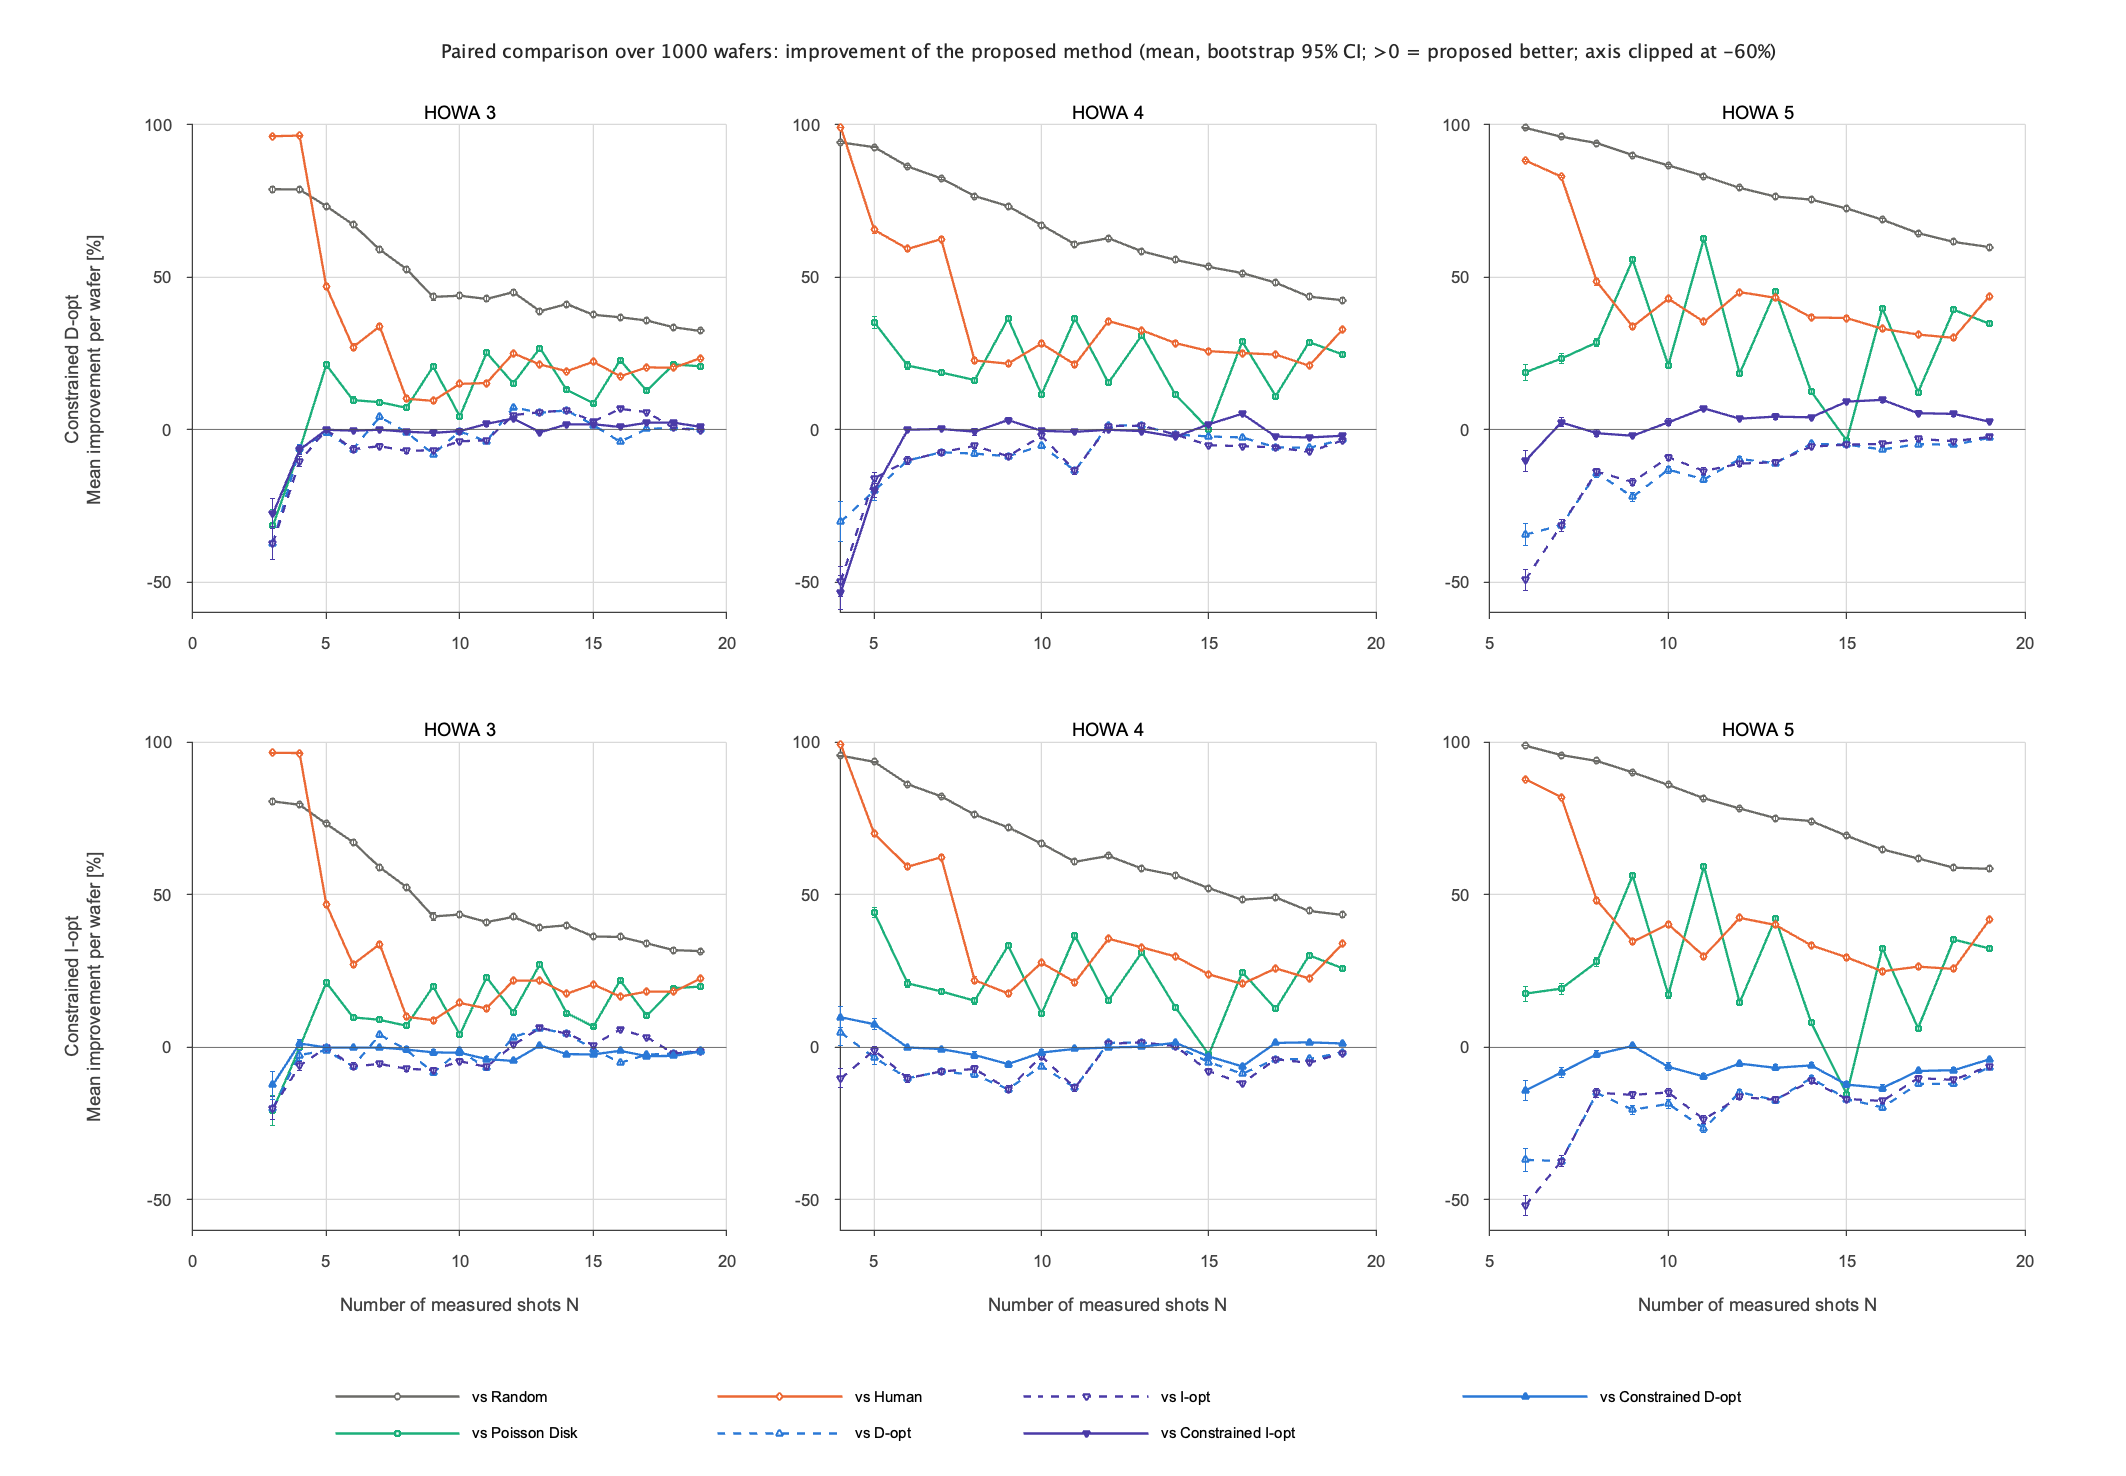
\includegraphics[width=\figw]{fig08_paired_improvement_base.png}
  \caption{提案法の改善率（waferごとの改善率の平均とbootstrap 95\%信頼区間）．上：C-D-opt，下：C-I-opt．}
  \label{fig:paired}
\end{figure}

\subsection{P95/P99/Worst case}
\label{sec:tail}

表\ref{tab:tail}に$N=12$でのtail指標を，図\ref{fig:tail}にshot数依存性を示す．
1000 waferの中でのばらつき（RMSのP95・最悪値）は平均値と同じ順位で，制約付き設計はHuman・Poissonより小さかった．
一方，wafer内の大きな残差（P99$|e|$・Max$|e|$）は，制約付き設計の方が制約なしのD/I最適より大きかった（5次でMax 4.45 vs 3.13\,nm）．

この差の場所を調べるため，評価点を候補shotのmark（228点，wafer内側）とpartial shotのmark（84点，外周）に分けた．
内側だけのRMSは，制約付き設計が制約なしより小さかった（$N=12$で3次0.85 vs 0.98，4次0.80 vs 0.90，5次0.81 vs 0.83\,nm）．
外周だけのRMS（waferごとの全体RMSと内側RMSから算出）は逆に大きかった（5次$N=12$でD-opt 1.19，C-D-opt 1.47\,nm）．
partial shotの領域は候補shotの外側にあり，補正は外挿になる．
制約付き設計は半径領域の上限により最外周のshot数が制限されるため，外挿の誤差が増え，その分だけwafer内側の誤差が減る．
内側だけで評価した場合の$N=8$〜19の改善率の中央値は，C-D-optのD-optに対して3次+5.8\%・4次+2.4\%・5次+2.7\%で，全評価点での結果（+0.9\%・$-3.8\%$・$-7.5\%$）と符号が変わる．
どちらの領域を重視するかは，製品のdie配置（外周のpartial shotに有効なdieがどれだけあるか）で決まる．

\begin{table}[htbp]
  \centering
  \caption{tail指標（$N=12$，nm）．平均〜最悪はwaferごとのRMSの1000 waferでの統計，P99$|e|$・Max$|e|$はwafer内の残差の大きさの99\%点・最大値の平均，内側RMSは候補shotのmarkだけのRMSの平均}
  \label{tab:tail}
  \small
\begin{tabular}{clrrrrrrr}
\toprule
次数 & 手法 & 平均 & 中央値 & P95 & 最悪 & P99$|e|$ & Max$|e|$ & 内側RMS \\
\midrule
\multirow{7}{*}{3} & Random & 1.90 & 1.85 & 2.72 & 3.97 & 6.26 & 7.34 & 1.32 \\
 & Poisson & 1.19 & 1.18 & 1.55 & 2.00 & 3.40 & 3.98 & 0.99 \\
 & Human & 1.36 & 1.34 & 1.85 & 2.54 & 4.47 & 5.18 & 0.97 \\
 & D-opt & 1.09 & 1.08 & 1.40 & 1.86 & 2.55 & 3.18 & 0.98 \\
 & I-opt & 1.06 & 1.05 & 1.35 & 1.79 & 2.67 & 3.37 & 0.91 \\
 & C-D-opt & 1.01 & 0.99 & 1.33 & 1.67 & 2.62 & 3.35 & 0.85 \\
 & C-I-opt & 1.05 & 1.03 & 1.39 & 1.78 & 3.00 & 3.72 & 0.87 \\
\midrule
\multirow{7}{*}{4} & Random & 2.73 & 2.66 & 3.91 & 5.21 & 9.32 & 11.71 & 1.76 \\
 & Poisson & 1.16 & 1.13 & 1.54 & 2.12 & 3.54 & 4.19 & 0.93 \\
 & Human & 1.55 & 1.51 & 2.12 & 3.00 & 5.48 & 6.37 & 1.00 \\
 & D-opt & 0.99 & 0.97 & 1.28 & 1.74 & 2.36 & 3.07 & 0.90 \\
 & I-opt & 0.99 & 0.97 & 1.29 & 1.62 & 2.36 & 3.07 & 0.90 \\
 & C-D-opt & 0.97 & 0.96 & 1.24 & 1.63 & 2.66 & 3.58 & 0.80 \\
 & C-I-opt & 0.97 & 0.96 & 1.24 & 1.63 & 2.66 & 3.58 & 0.80 \\
\midrule
\multirow{7}{*}{5} & Random & 5.56 & 5.22 & 9.06 & 14.41 & 25.00 & 31.80 & 2.99 \\
 & Poisson & 1.29 & 1.26 & 1.71 & 2.50 & 4.46 & 5.50 & 0.96 \\
 & Human & 1.94 & 1.90 & 2.65 & 4.46 & 7.64 & 9.01 & 1.16 \\
 & D-opt & 0.95 & 0.94 & 1.18 & 1.68 & 2.35 & 3.13 & 0.83 \\
 & I-opt & 0.93 & 0.92 & 1.17 & 1.64 & 2.32 & 3.06 & 0.82 \\
 & C-D-opt & 1.03 & 1.02 & 1.30 & 1.72 & 3.18 & 4.45 & 0.81 \\
 & C-I-opt & 1.08 & 1.06 & 1.39 & 1.91 & 3.59 & 4.60 & 0.82 \\
\bottomrule
\end{tabular}
\end{table}

\begin{figure}[htbp]
  \centering
  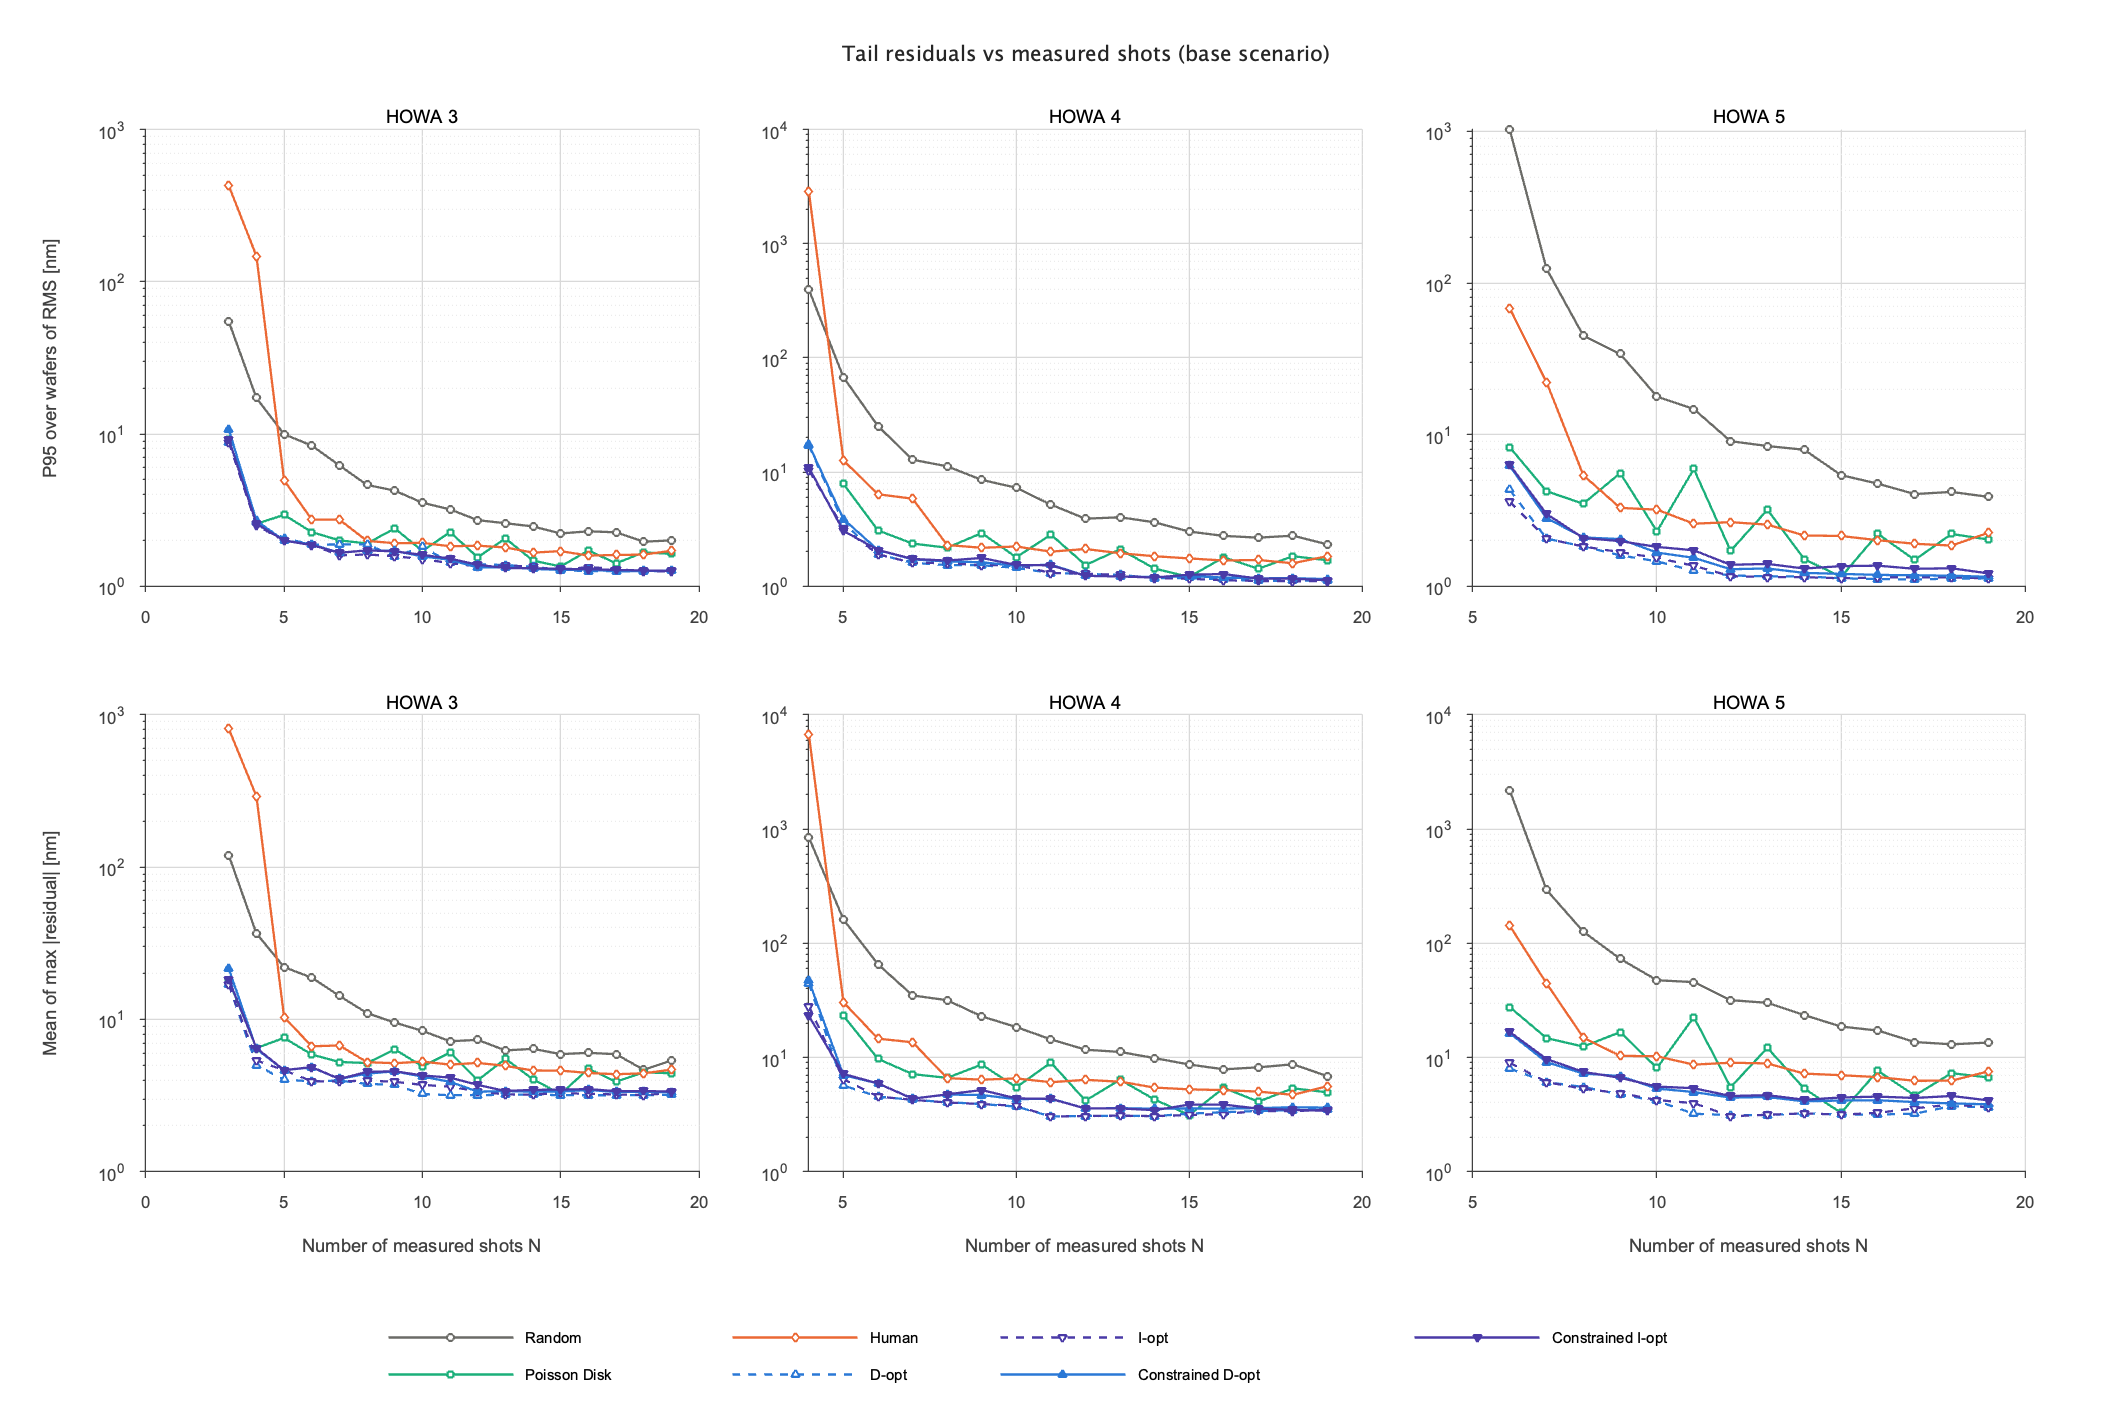
\includegraphics[width=\figw]{fig04_tail_vs_shots_base.png}
  \caption{tail指標のshot数依存性（上：waferごとのRMSのP95，下：wafer内最大残差の平均）．}
  \label{fig:tail}
\end{figure}

\subsection{scan-direction noise robustness}

表\ref{tab:robust}と図\ref{fig:robust}に，scan方向依存成分の倍率を変えたときの平均RMSを示す（$N=12$）．
scan成分が大きいほど，制約付き設計（scan方向を均等化）と制約なしの差は提案法に有利な方向へ動いた．
$N=12$のC-D-optのD-optに対する改善率は，3次でscan成分0倍$-1.0\%$，1倍+7.4\%，2倍+16.1\%，4倍+22.7\%，4次で$-1.3\%$・+2.2\%・+4.8\%・+6.2\%，5次で$-15.6\%$・$-8.9\%$・$-3.6\%$・$-0.5\%$だった．
ただし効果は一様ではなく，3次$N=8$では4倍でも$-14.2\%$と制約付き設計の方が悪かった．
scan方向の数をそろえても，Up/Downが列ごとに交互になるパターンが多項式に写り込む量はshotの位置で変わるためであり，数の均等化だけではscan成分の影響を消せない．

\subsection{measurement noise robustness}

mark計測誤差を0.25・0.5・1.0\,nmにすると，全手法で残差が増えたが順位は変わらなかった（表\ref{tab:robust}）．
5次では誤差が大きいほど制約付き設計の不利が広がった（$N=12$で$-6.5\%$→$-8.9\%$→$-12.4\%$）．
D/I-efficiencyが低い（誤差を増幅しやすい）設計の弱点が，誤差が大きいほど表に出るためである．
3次では逆に縮んだ（+8.3\%→+7.4\%→+5.0\%）．3次ではモデル不一致（バイアス）が残差の主成分で，誤差が大きくなると分散の寄与が増え，D-optの分散の小ささが効いてくる．

\begin{table}[htbp]
  \centering
  \caption{mark計測誤差（1σ, nm）とscan方向依存成分の倍率を変えたときの平均RMS [nm]（$N=12$）}
  \label{tab:robust}
  \small
\begin{tabular}{clrrrrrrr}
\toprule
次数 & 手法 & 誤差0.25 & 0.5 & 1.0 & scan×0 & ×0.5 & ×2 & ×4 \\
\midrule
\multirow{6}{*}{3} & Poisson & 1.15 & 1.19 & 1.36 & 1.00 & 1.05 & 1.63 & 2.74 \\
 & Human & 1.30 & 1.36 & 1.58 & 1.15 & 1.21 & 1.85 & 3.11 \\
 & D-opt & 1.05 & 1.09 & 1.23 & 0.88 & 0.94 & 1.54 & 2.65 \\
 & I-opt & 1.02 & 1.06 & 1.21 & 0.88 & 0.93 & 1.45 & 2.45 \\
 & C-D-opt & 0.96 & 1.01 & 1.17 & 0.89 & 0.92 & 1.29 & 2.05 \\
 & C-I-opt & 1.00 & 1.05 & 1.21 & 0.92 & 0.95 & 1.36 & 2.20 \\
\midrule
\multirow{6}{*}{4} & Poisson & 1.05 & 1.16 & 1.51 & 0.95 & 1.01 & 1.63 & 2.81 \\
 & Human & 1.41 & 1.55 & 2.00 & 1.24 & 1.32 & 2.24 & 3.93 \\
 & D-opt & 0.92 & 0.99 & 1.23 & 0.77 & 0.84 & 1.46 & 2.57 \\
 & I-opt & 0.92 & 0.99 & 1.23 & 0.77 & 0.83 & 1.45 & 2.56 \\
 & C-D-opt & 0.89 & 0.97 & 1.24 & 0.78 & 0.83 & 1.39 & 2.41 \\
 & C-I-opt & 0.89 & 0.97 & 1.24 & 0.78 & 0.83 & 1.39 & 2.41 \\
\midrule
\multirow{6}{*}{5} & Poisson & 1.08 & 1.29 & 1.89 & 1.10 & 1.15 & 1.73 & 2.87 \\
 & Human & 1.62 & 1.94 & 2.88 & 1.65 & 1.72 & 2.63 & 4.43 \\
 & D-opt & 0.83 & 0.95 & 1.31 & 0.72 & 0.78 & 1.42 & 2.54 \\
 & I-opt & 0.81 & 0.93 & 1.30 & 0.72 & 0.78 & 1.38 & 2.47 \\
 & C-D-opt & 0.88 & 1.03 & 1.48 & 0.83 & 0.88 & 1.47 & 2.56 \\
 & C-I-opt & 0.93 & 1.08 & 1.53 & 0.88 & 0.93 & 1.52 & 2.63 \\
\bottomrule
\end{tabular}
\end{table}

\begin{figure}[htbp]
  \centering
  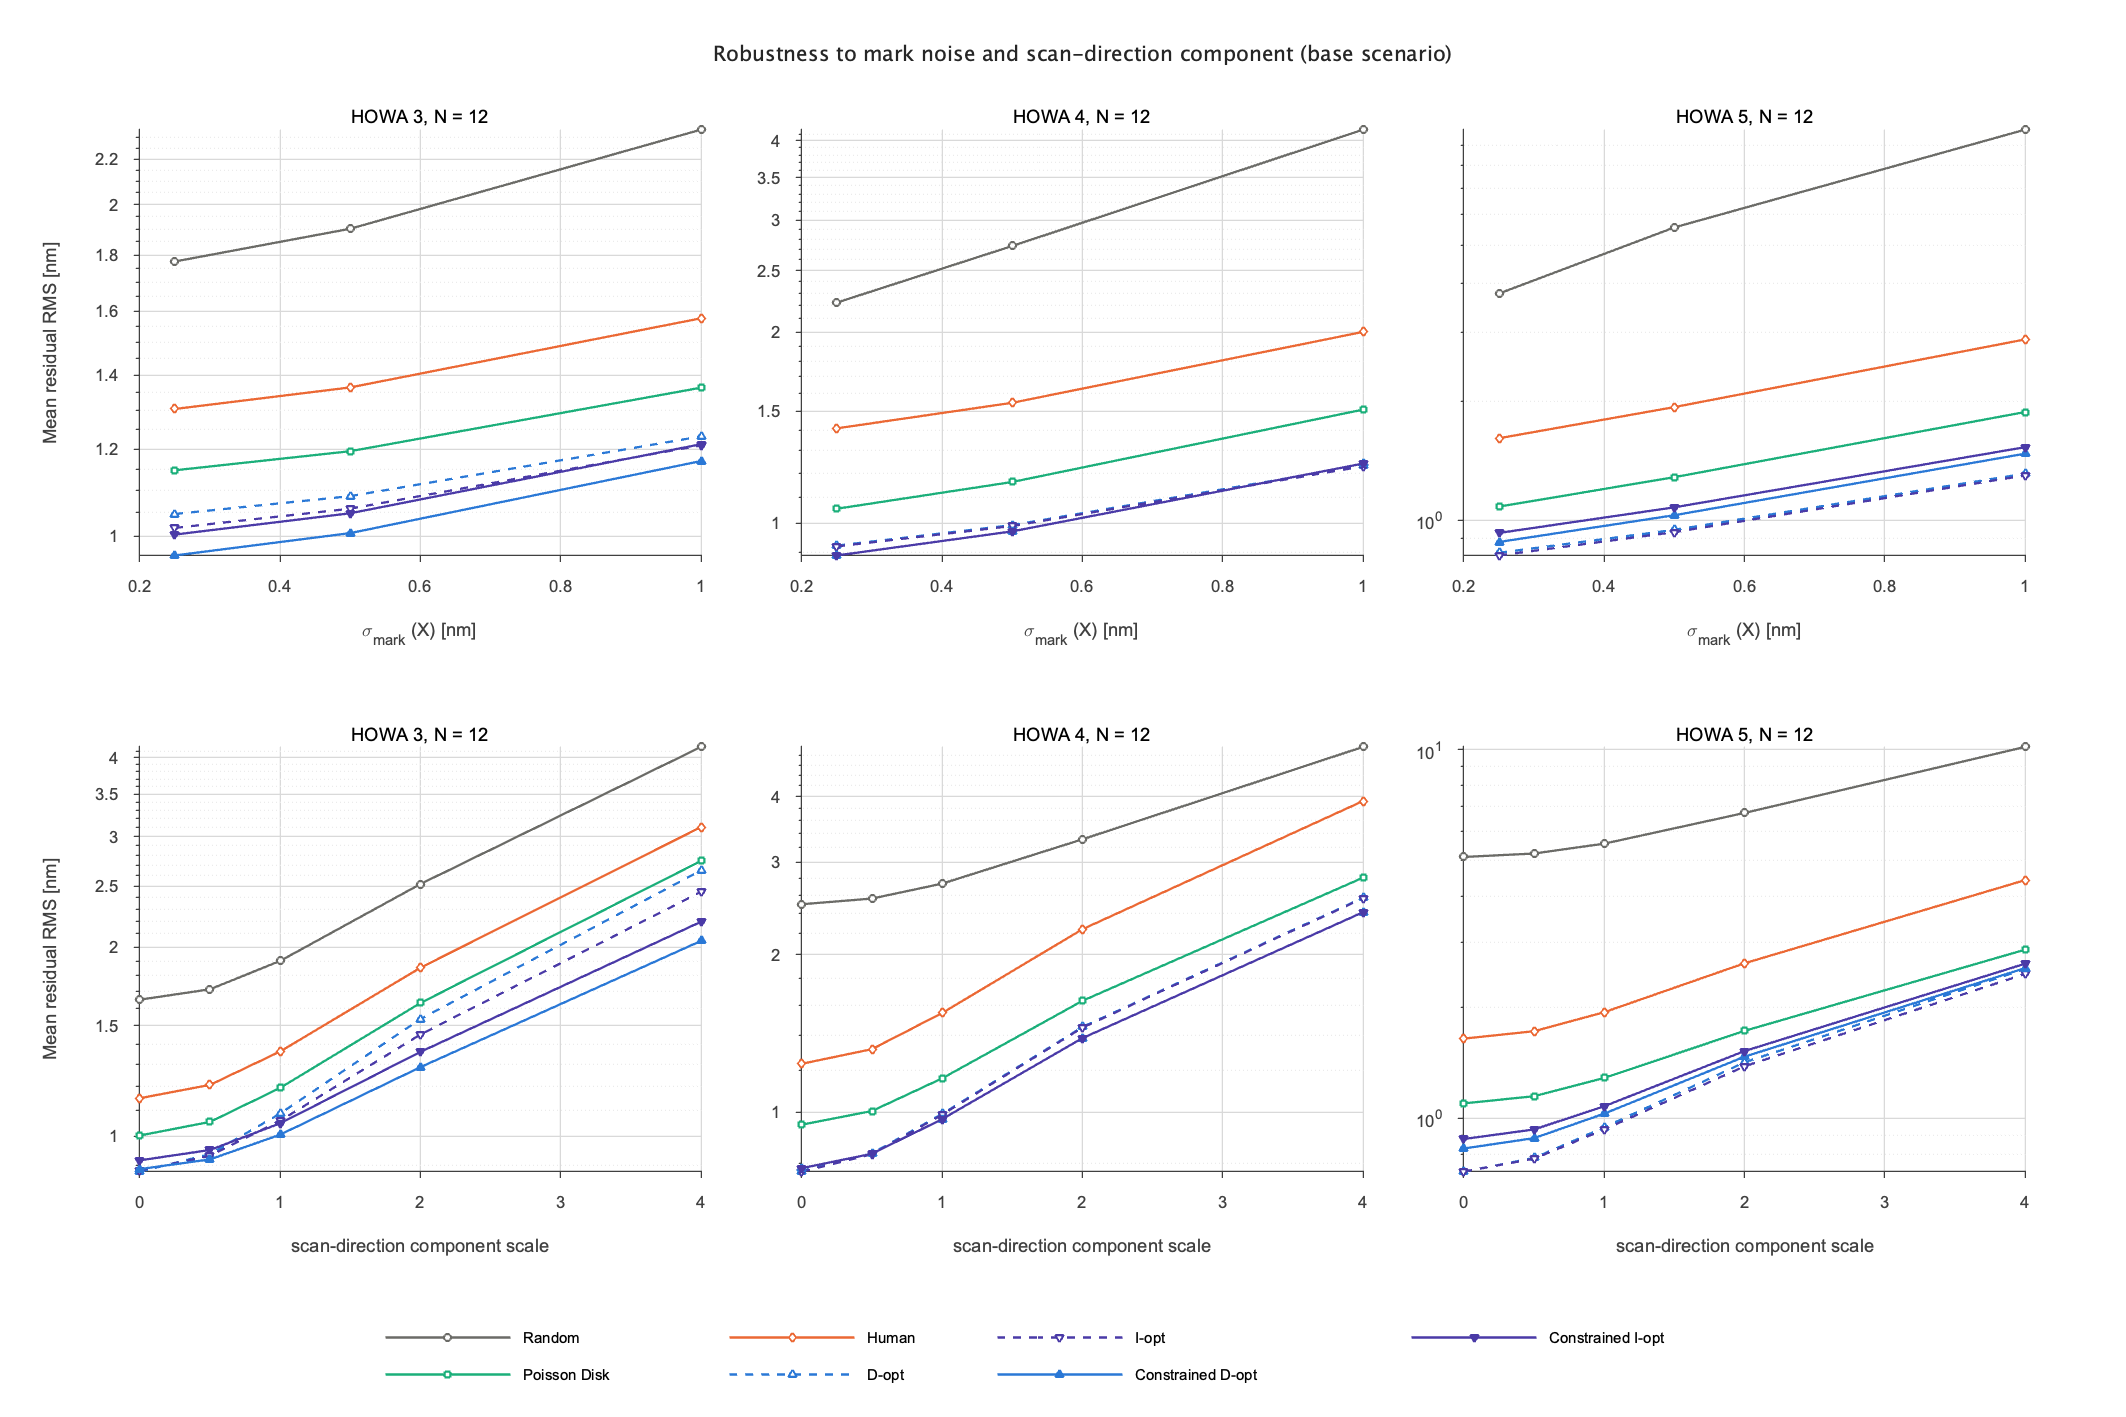
\includegraphics[width=\figw]{fig09_robustness_base_N12.png}
  \caption{mark計測誤差（上）とscan方向依存成分の倍率（下）に対する平均RMS（$N=12$）．}
  \label{fig:robust}
\end{figure}

\subsection{mandatory shot影響}

表\ref{tab:mand}に強制計測shotありの平均RMSを示す．
強制shot 5 shot（中心＋十字，うち4 shotがMiddle）を固定すると，同じ$N$の強制shotなしの制約付き設計より残差が大きくなった．
C-D-opt Augmentationの強制shotなしC-D-optに対する比は，5次で$N=7$ 8.0倍，$N=9$ 3.1倍，$N=12$ 1.30倍，$N=19$ 0.97倍で，3次・4次も$N\approx17$〜19で差がほぼなくなった．
少ないshot数では，強制shotが計測の大部分を占めて外周のshotを置けないためである．
さらに，強制shotと制約（Middleの上限・Innerの下限・scan方向）が重なると選べるshotが少なく，制約なしの拡張計画（D-opt Aug）との差が大きい（5次$N=9$で4.56 vs 1.59\,nm）．
6 shotではMiddleの上限（3）を強制shotだけで超えるため，制約付きの設計は存在しなかった．

\begin{table}[htbp]
  \centering
  \caption{強制計測shotありの平均RMS [nm]（「rank不足」は設計が full rank でなく推定できないもの．右の2列は同じ$N$の強制shotなしの制約付き設計）}
  \label{tab:mand}
  \scriptsize
  \setlength{\tabcolsep}{3.5pt}
\begin{tabular}{crrrrrrrrrr}
\toprule
次数 & $N$ & Random+F & Human+F & D-opt Aug & C-D Naive & C-I Naive & C-D Aug & C-I Aug & C-D（Fなし） & C-I（Fなし） \\
\midrule
\multirow{7}{*}{3} & 7 & 2.57 & 2.34 & 1.96 & 1.96 & 2.44 & 1.96 & 1.96 & 1.28 & 1.28 \\
 & 8 & 2.44 & 2.40 & 1.46 & 2.07 & 2.07 & 1.56 & 1.51 & 1.30 & 1.30 \\
 & 9 & 2.29 & 2.03 & 1.19 & 1.59 & 1.59 & 1.46 & 1.46 & 1.28 & 1.28 \\
 & 10 & 2.13 & 1.73 & 1.22 & 1.43 & 1.56 & 1.37 & 1.37 & 1.20 & 1.21 \\
 & 12 & 1.96 & 1.43 & 1.14 & 1.24 & 1.24 & 1.18 & 1.17 & 1.01 & 1.05 \\
 & 15 & 1.74 & 1.26 & 1.02 & 1.07 & 1.09 & 1.04 & 1.06 & 0.96 & 0.98 \\
 & 19 & 1.43 & 1.22 & 0.93 & 0.97 & 0.96 & 0.96 & 0.97 & 0.94 & 0.95 \\
\midrule
\multirow{7}{*}{4} & 7 & 4.62 & 3.92 & 2.95 & rank不足 & 4.76 & 3.27 & 3.25 & 1.30 & 1.31 \\
 & 8 & 4.00 & 3.80 & 1.95 & 2.33 & 3.27 & 2.27 & 2.27 & 1.26 & 1.27 \\
 & 9 & 3.63 & 2.88 & 1.23 & 2.09 & 2.41 & 1.89 & 1.93 & 1.23 & 1.29 \\
 & 10 & 3.27 & 2.24 & 1.18 & 1.68 & 2.09 & 1.48 & 1.48 & 1.15 & 1.15 \\
 & 12 & 2.78 & 1.62 & 1.11 & 1.28 & 1.28 & 1.18 & 1.16 & 0.97 & 0.97 \\
 & 15 & 2.18 & 1.50 & 0.93 & 1.02 & 1.03 & 1.01 & 1.05 & 0.94 & 0.97 \\
 & 19 & 1.80 & 1.29 & 0.84 & 0.88 & 0.88 & 0.89 & 0.88 & 0.89 & 0.87 \\
\midrule
\multirow{7}{*}{5} & 7 & 22.47 & 10.89 & 9.15 & rank不足 & 17.12 & 15.85 & 13.05 & 1.97 & 2.08 \\
 & 8 & 13.48 & 10.43 & 4.82 & 16.24 & 16.98 & 12.05 & 6.85 & 1.56 & 1.56 \\
 & 9 & 9.89 & 5.56 & 1.59 & 15.74 & 7.77 & 4.56 & 4.60 & 1.48 & 1.46 \\
 & 10 & 8.41 & 4.77 & 1.43 & 3.20 & 3.13 & 2.28 & 2.26 & 1.26 & 1.32 \\
 & 12 & 5.59 & 2.38 & 1.16 & 1.64 & 1.66 & 1.34 & 1.39 & 1.03 & 1.08 \\
 & 15 & 4.11 & 1.88 & 0.90 & 1.10 & 1.10 & 1.08 & 1.12 & 0.95 & 1.06 \\
 & 19 & 2.55 & 1.56 & 0.86 & 0.86 & 0.92 & 0.87 & 0.92 & 0.90 & 0.93 \\
\bottomrule
\end{tabular}
\end{table}

\subsection{augmentation効果}

強制shotの情報量を考慮する拡張計画（Augmentation）と，考慮しない素朴な方法（Naive）を比べた（図\ref{fig:aug}）．
Naiveは，4次・5次の$N=7$（追加2 shot）で設計がrank不足になり，補正係数を推定できなかった（C-D Naive）．
強制shotの情報を無視して追加shotを選ぶと，強制shotと合わせたときに情報が足りない方向が残るためである．
Augmentationは全shot数でfull rankだった．
推定できた範囲の平均RMSの改善率（Augmentation対Naive）は，5次で$N=8$ +25.8\%（C-D）／+59.6\%（C-I），$N=9$ +71.0\%／+40.8\%，$N=10$ +28.6\%／+27.6\%，$N=12$ +17.9\%／+16.4\%，4次で$N=10$ +11.7\%／+29.1\%，$N=12$ +8.2\%／+9.2\%，3次で$N=8$ +25.0\%／+26.7\%，$N=12$ +4.5\%／+5.8\%で，いずれもbootstrap信頼区間が0を上回った．
$N\ge13$では差は概ね$\pm5\%$以内で，NaiveとAugmentationが同じ設計になるshot数もあった．一部で有意にNaiveが良い点（5次$N=18$のC-I $-11.4\%$など）もあり，交換法の局所解による揺れと考えられる．
強制shotの割合が大きい（追加shotが少ない）ほど，固定shotの情報量を考慮する意義が大きい．

\begin{figure}[htbp]
  \centering
  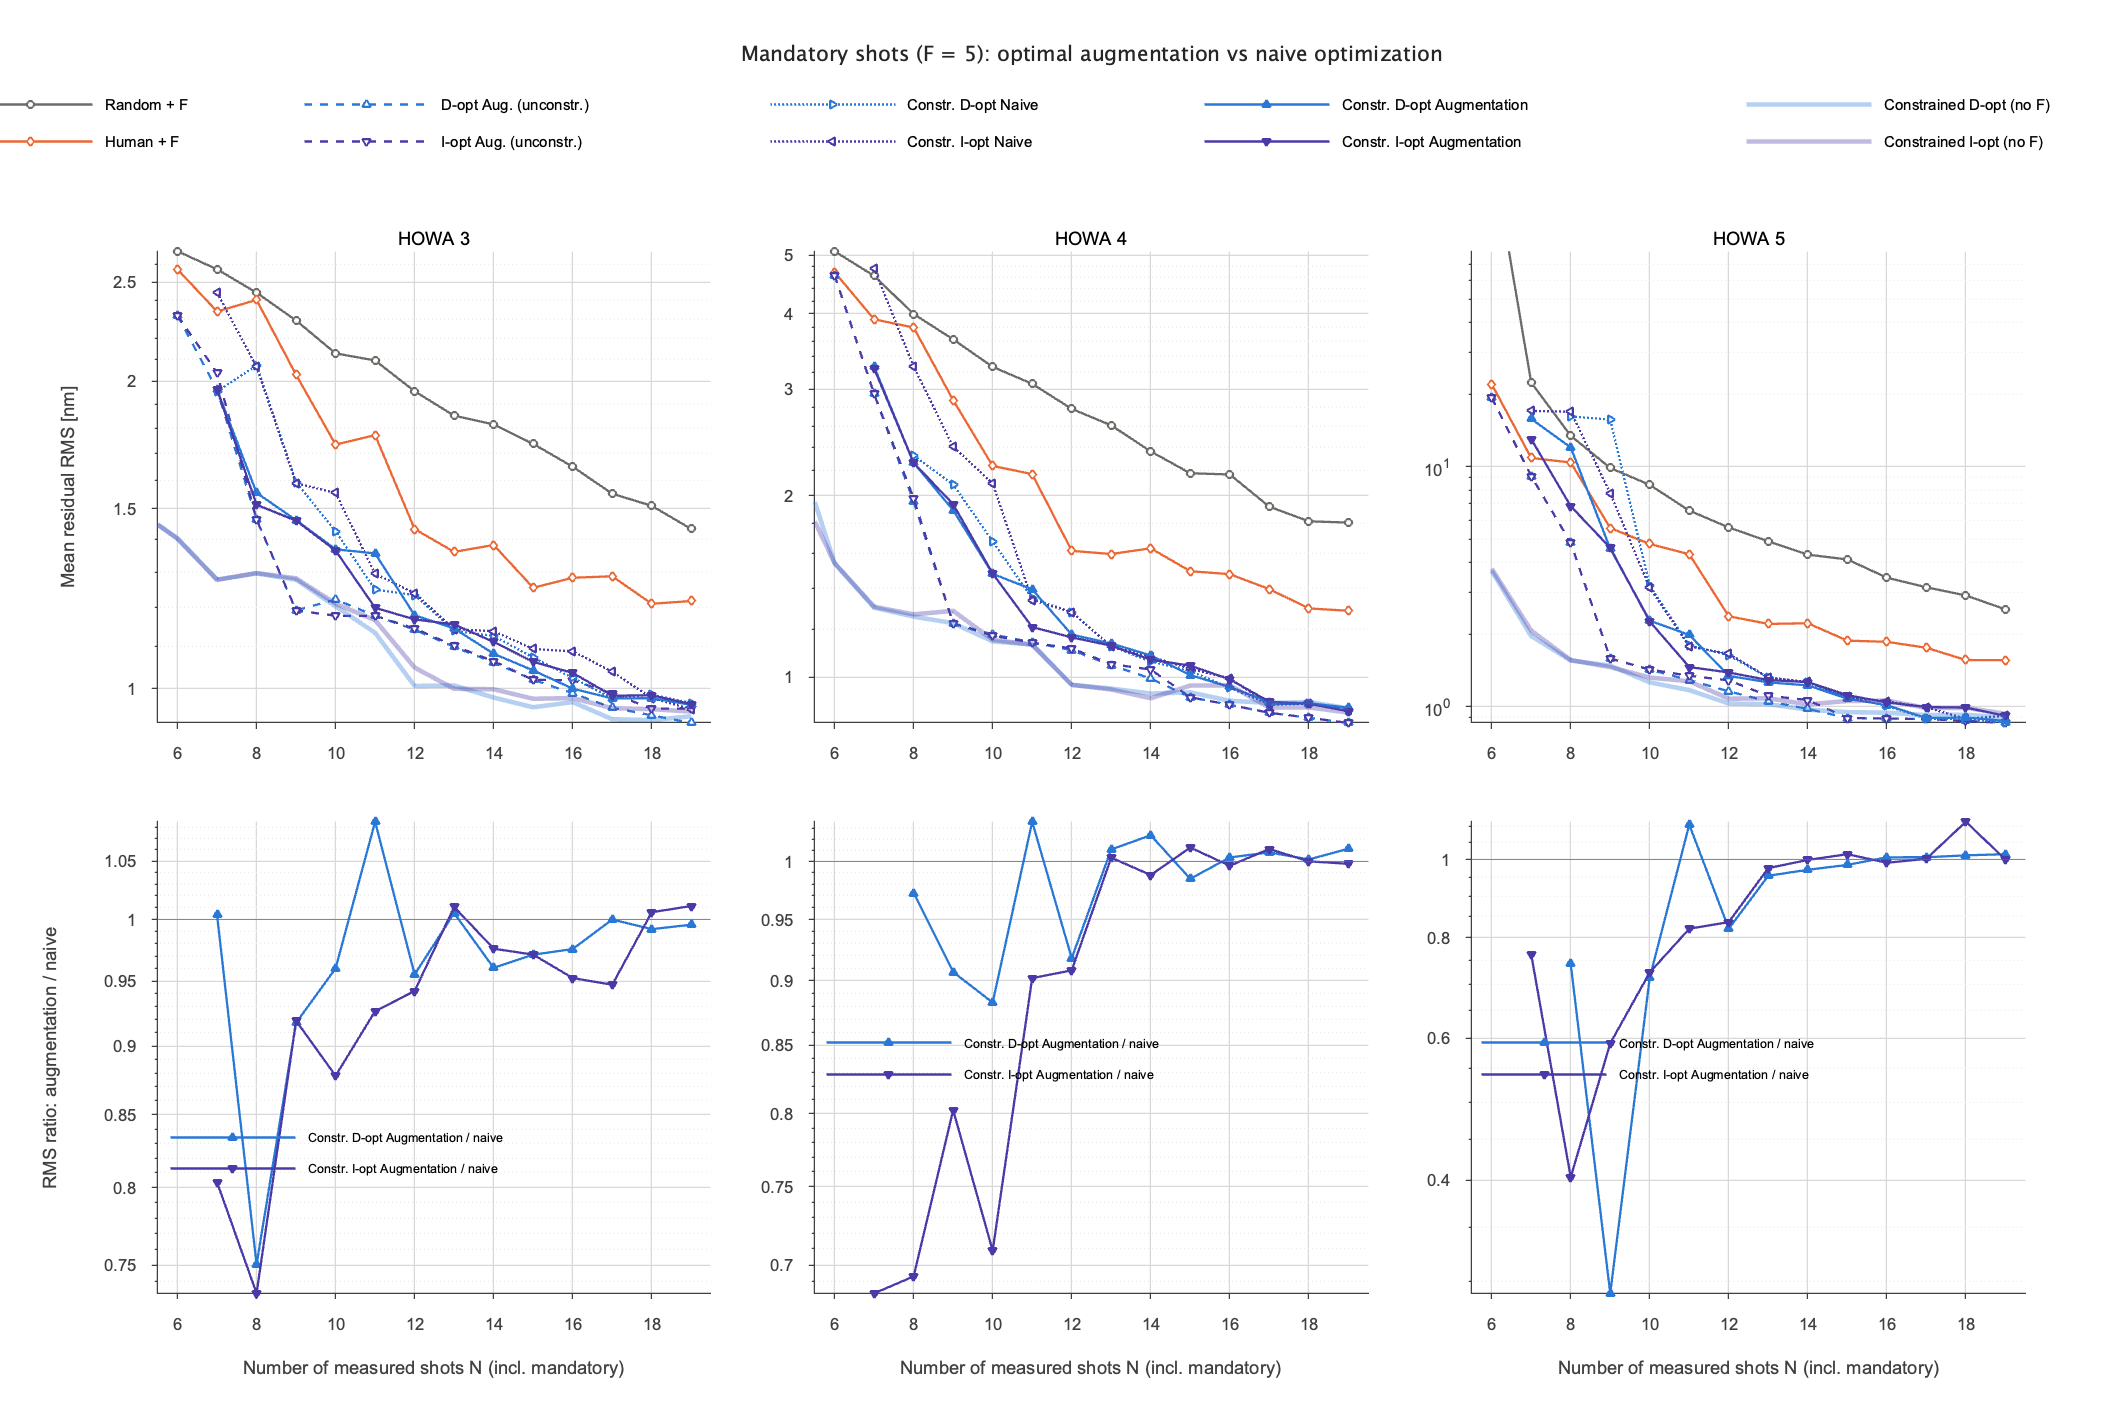
\includegraphics[width=\figw]{fig12_augmentation.png}
  \caption{強制計測shotあり．上：平均RMS（太い薄線は強制shotなしの制約付き設計），下：AugmentationとNaiveの平均RMSの比（1未満ならAugmentationが良い）．}
  \label{fig:aug}
\end{figure}

\subsection{measured shot数依存性}

図\ref{fig:rms}のとおり，最適化した設計の残差は$N_\text{min}$から急に下がり，3次では$N\approx5$，4次では$N\approx8$，5次では$N\approx11$〜12で傾きが緩やかになった．
これは計測mark数$4N$が項数の約2倍（3次20，4次30，5次42）に達するあたりである．
$N=19$でも3次0.94，4次0.86，5次0.88\,nmで，モデル不一致の下限（0.77・0.55・0.39\,nm）との差は，計測誤差とscan成分による推定誤差である．
Poissonの残差はshot数に対して単調でなかった（5次で$N=12$ 1.29，$N=13$ 2.02，$N=15$ 0.92\,nm）．
Poissonは点の間隔だけで選ぶため，最外周の候補を含むかどうかが$N$ごとに変わり，外挿の精度が大きく変わるためである．

\subsection{Human Sampling比較}

Humanと同じ平均RMSを得るのに必要な最小shot数を表\ref{tab:reduction}と図\ref{fig:reduction}に示す．
Humanの12 shotと同じ平均RMSは，C-D-optでは3次7・4次6・5次8 shotで得られ，計測shot数を42\%・50\%・33\%減らせる．
Humanの19 shotに対しては10・7・8 shot（47\%・63\%・58\%削減）だった．
制約なしのD-optはさらに少ない（12 shotに対して6・6・7 shot）が，前述のとおり制約を満たさない．
waferごとのRMSのP95（悪い側の5\%）を目標にしても，削減shot数はほぼ同じだった．
強制計測shotありでは，Human+Fの19 shotと同じ平均RMSを，C-I-opt Augmentationは11 shot（42\%削減），C-D-opt Augmentationは12 shot（37\%削減），Naiveは12〜13 shotで得た．

\begin{table}[htbp]
  \centering
  \caption{Humanと同じ平均RMSに必要な最小shot数（強制計測shotなし）．括弧内はHumanのshot数に対する削減率}
  \label{tab:reduction}
  \small
\begin{tabular}{crrrrrr}
\toprule
次数 & Human の $N$（目標RMS） & Poisson & D-opt & I-opt & C-D-opt & C-I-opt \\
\midrule
\multirow{4}{*}{3} & 8（1.47\,nm） & 7（+12\%） & 6（+25\%） & 6（+25\%） & 6（+25\%） & 6（+25\%） \\
 & 12（1.36\,nm） & 10（+17\%） & 6（+50\%） & 6（+50\%） & 7（+42\%） & 7（+42\%） \\
 & 15（1.24\,nm） & 12（+20\%） & 9（+40\%） & 7（+53\%） & 10（+33\%） & 10（+33\%） \\
 & 19（1.24\,nm） & 12（+37\%） & 9（+53\%） & 7（+63\%） & 10（+47\%） & 10（+47\%） \\
\midrule
\multirow{4}{*}{4} & 8（1.67\,nm） & 7（+12\%） & 6（+25\%） & 6（+25\%） & 6（+25\%） & 6（+25\%） \\
 & 12（1.55\,nm） & 8（+33\%） & 6（+50\%） & 6（+50\%） & 6（+50\%） & 6（+50\%） \\
 & 15（1.30\,nm） & 12（+20\%） & 7（+53\%） & 7（+53\%） & 8（+47\%） & 8（+47\%） \\
 & 19（1.35\,nm） & 10（+47\%） & 7（+63\%） & 7（+63\%） & 7（+63\%） & 7（+63\%） \\
\midrule
\multirow{4}{*}{5} & 8（3.31\,nm） & 7（+12\%） & 6（+25\%） & 6（+25\%） & 7（+12\%） & 7（+12\%） \\
 & 12（1.94\,nm） & 10（+17\%） & 7（+42\%） & 7（+42\%） & 8（+33\%） & 8（+33\%） \\
 & 15（1.54\,nm） & 12（+20\%） & 7（+53\%） & 7（+53\%） & 9（+40\%） & 9（+40\%） \\
 & 19（1.65\,nm） & 12（+37\%） & 7（+63\%） & 7（+63\%） & 8（+58\%） & 8（+58\%） \\
\bottomrule
\end{tabular}
\end{table}

\begin{figure}[htbp]
  \centering
  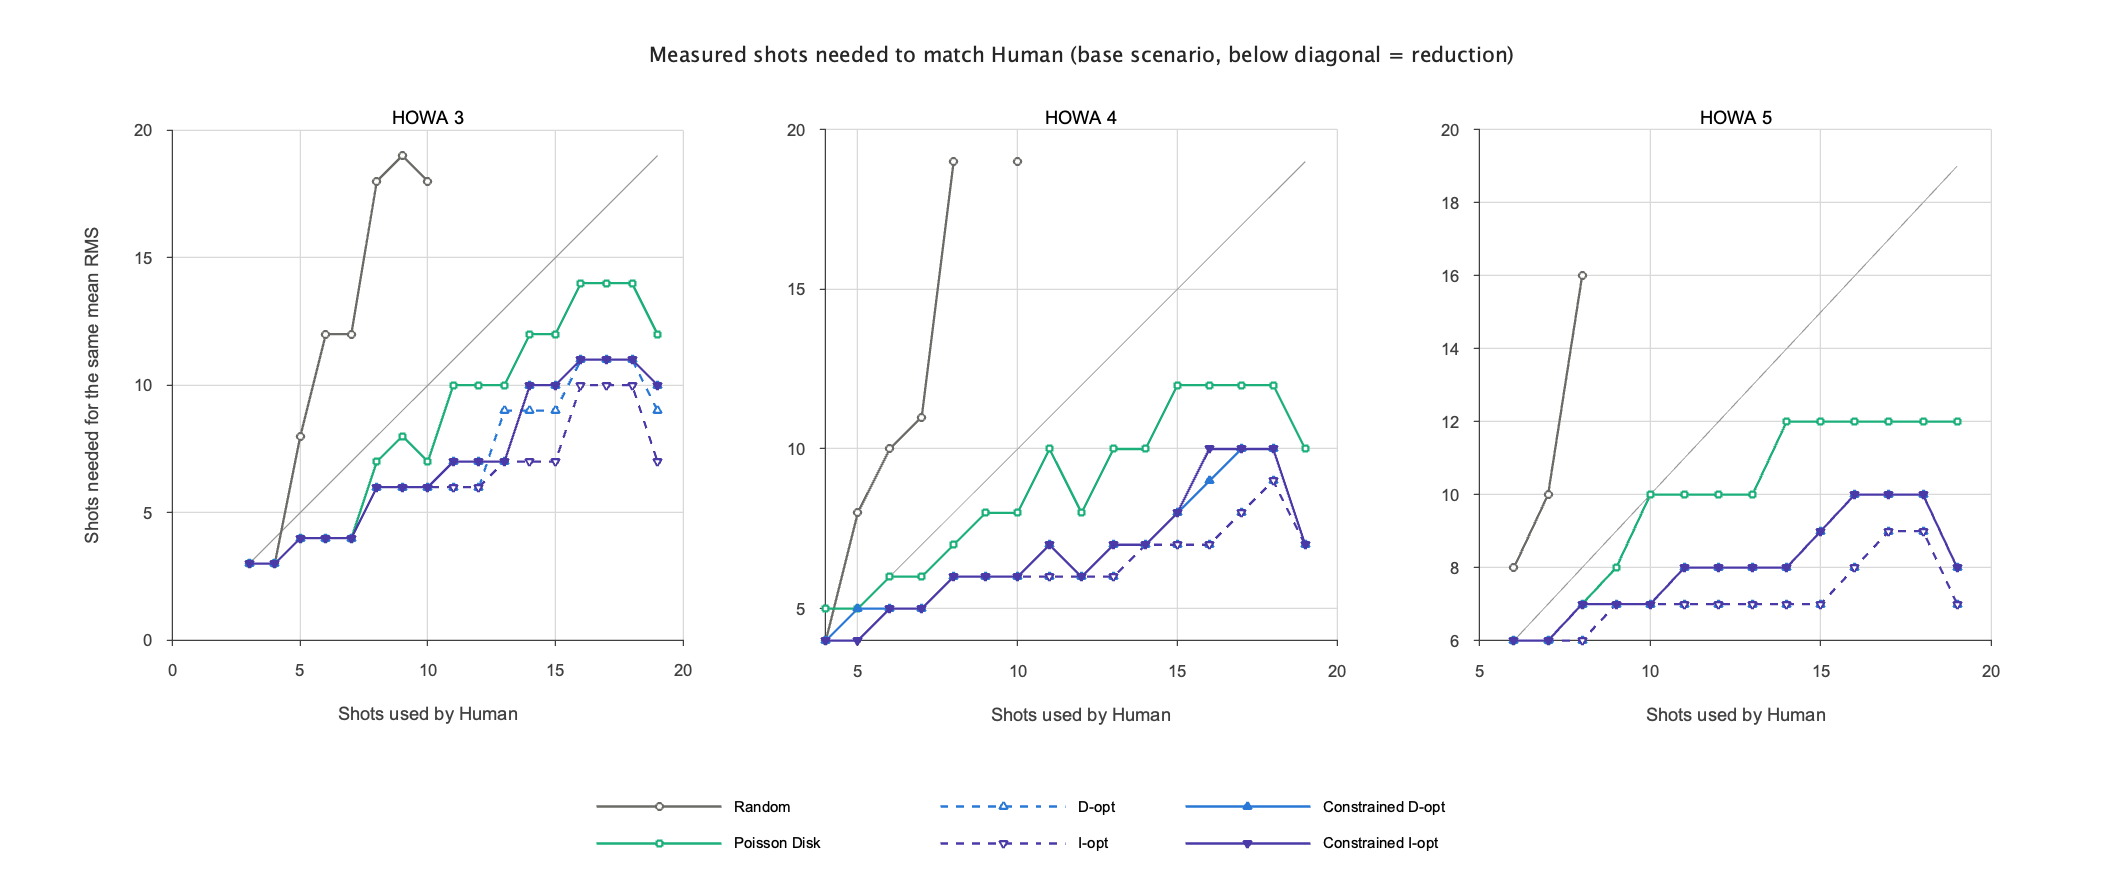
\includegraphics[width=\figw]{fig10_shot_reduction_base.png}
  \caption{Humanと同じ平均RMSに必要なshot数．対角線より下なら計測shot数を減らせる．}
  \label{fig:reduction}
\end{figure}

\subsection{計算時間と局所解依存性}
\label{sec:time}

設計1件（multi-start 201回の合計）の計算時間を表\ref{tab:time}に示す．
D基準は平均1〜2秒，I基準は逆行列の計算が加わるため長く，5次では平均11秒（最大16秒）だった．
制約付き設計は，交換できる候補が上下限で絞られるため制約なしより短い．
本計算全体（設計618件，Random 89組×200抽選，7条件×707設計×1000 waferの評価，統計，soft制約の補助評価，図）の所要時間は約33分で，内訳は設計12.9分，Monte Carlo評価4.6分，統計2.4分，soft制約の補助評価9.7分，図3.4分だった（\texttt{results/logs/timing\_log.csv}）．

局所解への依存性を，各設計で最良値（相対差$10^{-6}$以内）に到達した初期解の割合で調べた．
中央値は，制約なしのD/I最適で0.4〜0.8だったのに対し，制約付きでは0.03〜0.11と小さく，制約付き問題は局所解が多い．
そこでmulti-start回数の妥当性を，制約付き設計（HOWA 3〜5次，$N=8$・12・19，D・I）の18条件について，20・100・200・400回の最良値を400回の最良値と比べて確認した（\texttt{tools/check\_multistart.m}，\texttt{results/csv/multistart\_check.csv}）．
20回では18条件中7条件で400回の最良値に届かず，効率が最大3.6\%低かった．100回でも3条件で最大3.4\%低かった．
200回では17条件で400回と同じ値になり，残る1条件（4次・$N=12$のI基準）も効率0.992だった．
本評価の200回（＋相互初期解1回）は，効率で1\%未満の差まで最良値に近い設計を得ていると考えられるが，大域最適の保証ではない．


\begin{table}[htbp]
  \centering
  \caption{設計1件（multi-start全体）の計算時間 [s]（平均 / 最大，MATLAB R2022b，Rosetta 2，並列化なし）}
  \label{tab:time}
  \small
\begin{tabular}{crrrrrrr}
\toprule
次数 & D-opt & I-opt & C-D-opt & C-I-opt & C-D Aug & C-I Aug & Poisson \\
\midrule
3 & 1.03 / 1.73 & 1.78 / 2.84 & 0.88 / 1.46 & 1.25 / 2.20 & 0.56 / 1.59 & 0.77 / 1.56 & 0.02 / 0.05 \\
4 & 1.16 / 1.79 & 2.30 / 3.57 & 0.96 / 1.70 & 1.55 / 2.90 & 0.58 / 1.55 & 0.90 / 1.84 & 0.01 / 0.03 \\
5 & 1.68 / 2.61 & 10.95 / 16.48 & 1.24 / 2.05 & 6.04 / 10.70 & 0.71 / 1.59 & 3.07 / 7.06 & 0.01 / 0.03 \\
\bottomrule
\end{tabular}
\end{table}

\subsection{soft制約の補助評価}
\label{sec:res-soft}

hard制約の代わりに罰則の重み$\lambda$を変えたsoft制約の結果を表\ref{tab:soft}と図\ref{fig:soft}に示す．
$\lambda=0.02$〜0.2の小さい罰則で，scan方向の違反は全条件で0になり，そのときのD-efficiencyは0.95以上だった．scan方向の均等化は，最適性をほとんど損なわずに満たせる制約である．
一方，半径領域の違反を0にするには$\lambda=0.1$〜2が必要で，そのときのD-efficiencyは0.86〜0.97，5次ではI-efficiencyが0.62〜0.75まで下がった．
平均RMSは，4次$N=12$のD基準で$\lambda=0.1$〜0.2（半径の違反2 shot，scan違反0）のとき0.95\,nmと，制約なし（0.99）・違反0（0.97〜0.99）より小さく，制約を少し緩めると最も良くなる場合もあった．
ただし$\lambda$に対する変化は単調でなく（交換法の局所解の影響），運用では$\lambda$を一つ決めて固定するより，hard制約で上下限を設定し直す方が扱いやすい．

\begin{table}[htbp]
  \centering
  \caption{soft制約の重み$\lambda$に対する「制約違反の合計 [shot] / 効率 / 平均RMS [nm]」（$\lambda=0$は制約なし．効率はD基準ならD-efficiency，I基準ならI-efficiencyで，$\lambda=0$のD/I最適が基準）}
  \label{tab:soft}
  \scriptsize
  \setlength{\tabcolsep}{3pt}
\begin{tabular}{crlcccccc}
\toprule
次数 & $N$ & 基準 & $\lambda=0$ & $\lambda=0.02$ & $\lambda=0.05$ & $\lambda=0.2$ & $\lambda=1$ & $\lambda=5$ \\
\midrule
3 & 8 & D & 10 / 1.00 / 1.31 & 2 / 0.99 / 1.25 & 2 / 0.99 / 1.25 & 2 / 0.99 / 1.25 & 0 / 0.91 / 1.30 & 0 / 0.91 / 1.30 \\
3 & 8 & I & 8 / 1.00 / 1.22 & 1 / 0.96 / 1.28 & 1 / 0.96 / 1.28 & 0 / 0.88 / 1.29 & 0 / 0.88 / 1.29 & 0 / 0.88 / 1.29 \\
3 & 12 & D & 14 / 1.00 / 1.09 & 10 / 0.99 / 1.06 & 2 / 0.97 / 1.02 & 0 / 0.95 / 1.01 & 0 / 0.95 / 1.01 & 0 / 0.95 / 1.01 \\
3 & 12 & I & 10 / 1.00 / 1.06 & 0 / 0.94 / 1.05 & 0 / 0.94 / 1.05 & 0 / 0.94 / 1.05 & 0 / 0.94 / 1.05 & 0 / 0.94 / 1.05 \\
3 & 19 & D & 8 / 1.00 / 0.94 & 1 / 1.00 / 0.94 & 1 / 1.00 / 0.94 & 1 / 1.00 / 0.94 & 0 / 0.97 / 0.94 & 0 / 0.97 / 0.94 \\
3 & 19 & I & 1 / 1.00 / 0.94 & 1 / 1.00 / 0.94 & 0 / 0.96 / 0.95 & 0 / 0.96 / 0.95 & 0 / 0.96 / 0.95 & 0 / 0.96 / 0.95 \\
\midrule
4 & 8 & D & 8 / 1.00 / 1.18 & 8 / 1.00 / 1.18 & 6 / 0.99 / 1.18 & 2 / 0.98 / 1.20 & 1 / 0.94 / 1.22 & 0 / 0.88 / 1.26 \\
4 & 8 & I & 10 / 1.00 / 1.21 & 1 / 0.97 / 1.23 & 1 / 0.97 / 1.23 & 0 / 0.83 / 1.26 & 0 / 0.83 / 1.27 & 0 / 0.83 / 1.27 \\
4 & 12 & D & 14 / 1.00 / 0.99 & 12 / 1.00 / 0.97 & 12 / 1.00 / 0.97 & 2 / 0.96 / 0.95 & 0 / 0.91 / 0.99 & 0 / 0.91 / 0.99 \\
4 & 12 & I & 14 / 1.00 / 0.99 & 2 / 0.92 / 0.95 & 0 / 0.85 / 0.97 & 0 / 0.85 / 0.97 & 0 / 0.84 / 1.02 & 0 / 0.84 / 1.02 \\
4 & 19 & D & 4 / 1.00 / 0.86 & 4 / 1.00 / 0.86 & 3 / 1.00 / 0.85 & 1 / 0.99 / 0.87 & 0 / 0.96 / 0.89 & 0 / 0.96 / 0.89 \\
4 & 19 & I & 4 / 1.00 / 0.86 & 1 / 1.00 / 0.87 & 1 / 1.00 / 0.87 & 0 / 0.94 / 0.87 & 0 / 0.94 / 0.88 & 0 / 0.94 / 0.87 \\
\midrule
5 & 8 & D & 8 / 1.00 / 1.39 & 8 / 1.00 / 1.38 & 8 / 1.00 / 1.38 & 2 / 0.97 / 1.46 & 1 / 0.93 / 1.45 & 0 / 0.86 / 1.56 \\
5 & 8 & I & 10 / 1.00 / 1.40 & 1 / 0.85 / 1.45 & 1 / 0.85 / 1.45 & 1 / 0.85 / 1.44 & 0 / 0.66 / 1.57 & 0 / 0.66 / 1.57 \\
5 & 12 & D & 12 / 1.00 / 0.95 & 12 / 1.00 / 0.95 & 10 / 1.00 / 0.93 & 2 / 0.95 / 0.96 & 0 / 0.89 / 1.03 & 0 / 0.89 / 1.03 \\
5 & 12 & I & 10 / 1.00 / 0.93 & 2 / 0.88 / 1.07 & 2 / 0.88 / 1.07 & 0 / 0.75 / 1.16 & 0 / 0.75 / 1.16 & 0 / 0.75 / 1.16 \\
5 & 19 & D & 3 / 1.00 / 0.88 & 1 / 1.00 / 0.88 & 1 / 1.00 / 0.88 & 1 / 1.00 / 0.88 & 0 / 0.96 / 0.90 & 0 / 0.96 / 0.90 \\
5 & 19 & I & 1 / 1.00 / 0.88 & 1 / 1.00 / 0.88 & 1 / 1.00 / 0.88 & 0 / 0.91 / 0.93 & 0 / 0.91 / 0.94 & 0 / 0.91 / 0.94 \\
\bottomrule
\end{tabular}
\end{table}

\begin{figure}[htbp]
  \centering
  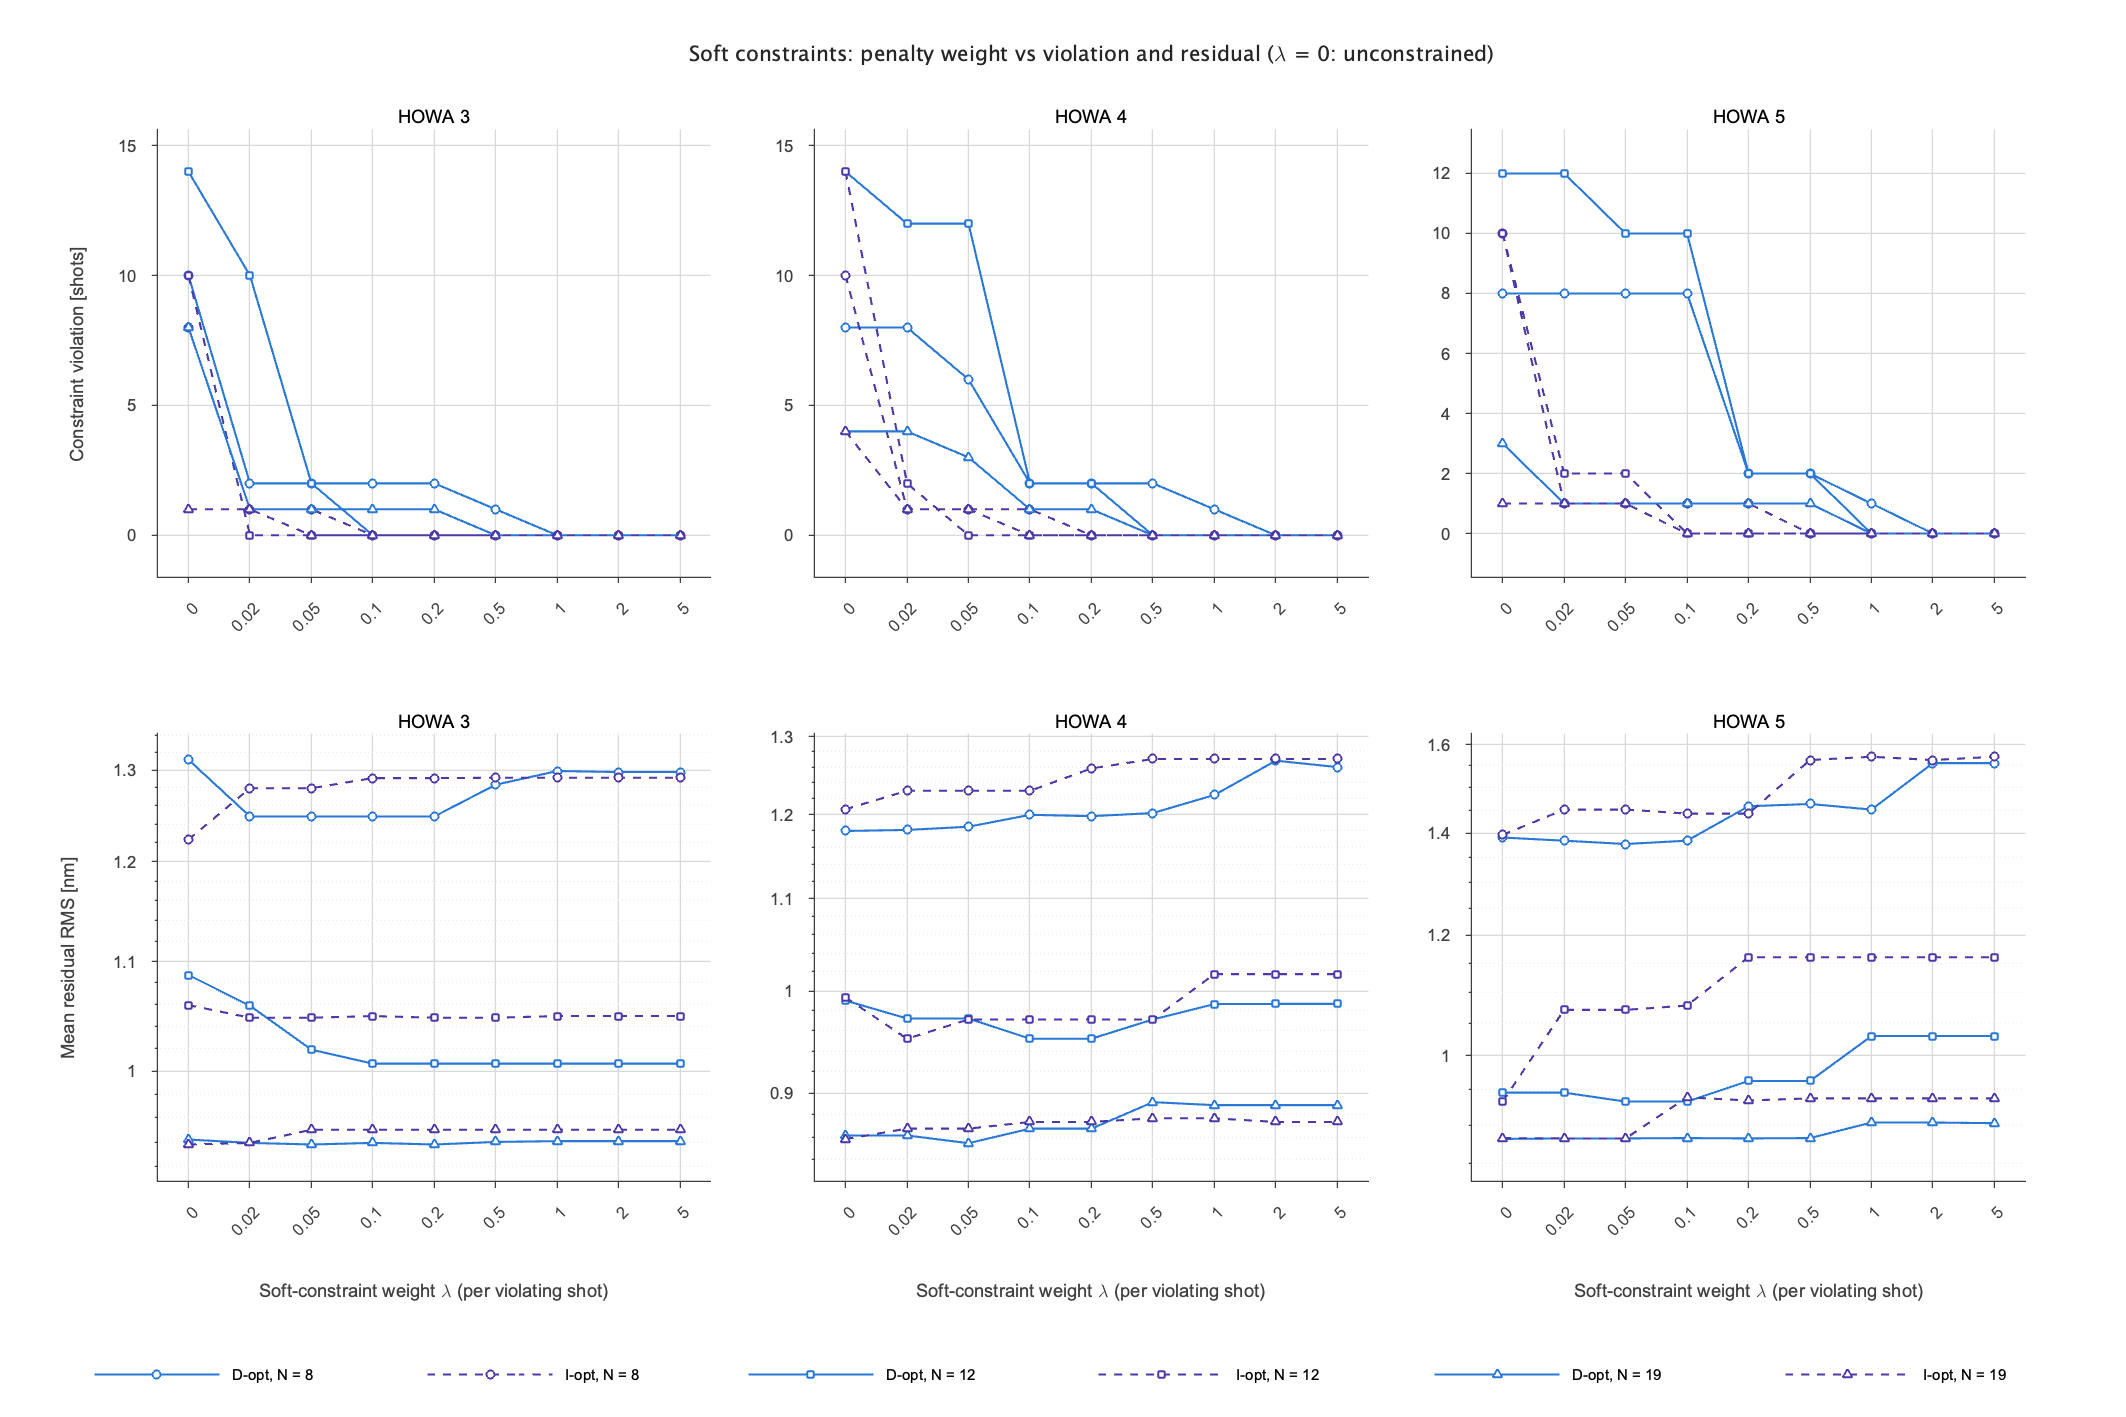
\includegraphics[width=\figw]{fig14_soft_constraint.png}
  \caption{soft制約の重みに対する制約違反（上）と平均RMS（下）．}
  \label{fig:soft}
\end{figure}

% ============================================================
\section{考察}
% ============================================================

\subsection{各sampling法の特徴}

\begin{description}
  \item[Random] 平均的にも，抽選ごとのばらつきの点でも最も悪い．HOWA 5次$N=12$では200抽選の平均RMSが最良1.51\,nm，中央値5.59\,nm，最悪348\,nmと，抽選しだいで補正が破綻する．
  \item[Poisson Disk] 空間的に均等で，D-efficiencyは0.6〜0.8と中程度．shot数によって最外周のshotを含むかどうかが変わり，残差が大きく上下する．
  \item[Human] 中心と2つの円の配置は象限が均等で直感的だが，外周の候補を十分に使わないため高次ほど不利で，D-efficiencyは0.44〜0.63にとどまる．
  \item[D-opt / I-opt] 平均RMSは最小に近いが，外周と中心に偏り，半径領域・scan方向の要求を満たさない．
  \item[Constrained D/I-opt] 制約を必ず満たし，Random・Poisson・Humanより大幅に良い．制約なしとの差は次数とshot数で変わる．
\end{description}

\subsection{D-optとI-optの違い}

本条件では，D最適とI最適の設計はよく似ており（$N\ge8$でD-optのI-efficiency 0.84以上，I-optのD-efficiency 0.95以上），補正残差の差は4次・5次で$\pm4\%$以内，3次で$-7$〜$+11\%$と符号も一定しなかった．
I最適の評価領域$E$をusable領域全体（外周を含む）にしたため，両者とも外周を重視する似た配置になったと考えられる．
制約付きでは，5次でC-I-optがC-D-optより残差が大きい場合が多かった（$N=8$〜19の中央値で約5\%）．
制約付きI最適は初期解の3\%しか最良値に到達しておらず（\ref{sec:time}節），探索の難しさも影響している可能性がある．
I最適の評価領域を製品dieのある領域に限るなど，評価領域の選び方で両者の差は変わりうる．

\subsection{制約あり/なしの違い}

制約の効果は，(1)半径領域の下限によりInner・Middleにshotを置くことで，wafer内側の推定は良くなるが外周の外挿は悪くなる，(2)scan方向の均等化でscan方向依存成分の偏りが減る，の二つに分けて考えられる．
(1)は全評価点で見ると3次では得，4次・5次では損になった．高次ほど外周での多項式の変化が大きく，外周のshotを減らす損が大きいためである．
(2)はscan成分が大きいほど効き，scan成分が名目の2〜4倍では4次・5次でも制約なしとの差がほぼ0〜正になった．
scan方向の均等化はsoft制約の結果から最適性の損失がごく小さいことも分かったので，常に課してよい制約といえる．

\subsection{optimalityと実補正性能の関係}

図\ref{fig:tradeoff}に，効率と平均RMS（同じ$N$の制約なし最適に対する比）の関係を示す．
効率が低い設計ほど残差が大きい傾向ははっきりしており，効率0.5未満（Random・HumanのN小）では残差が2倍〜数十倍になった．
一方，効率0.85〜1.0の範囲では効率と残差の順位は一致しない．
3次で制約付き設計（D-efficiency約0.95）がD-opt（1.0）より残差が小さいのはその例で，D/I基準が計測誤差による分散だけを見ており，モデル不一致によるバイアスとscan成分の写り込みを含まないためである．
最適性の数値は設計の良し悪しの目安になるが，最終的な判断には補正後の残差による評価が必要である．

\begin{figure}[htbp]
  \centering
  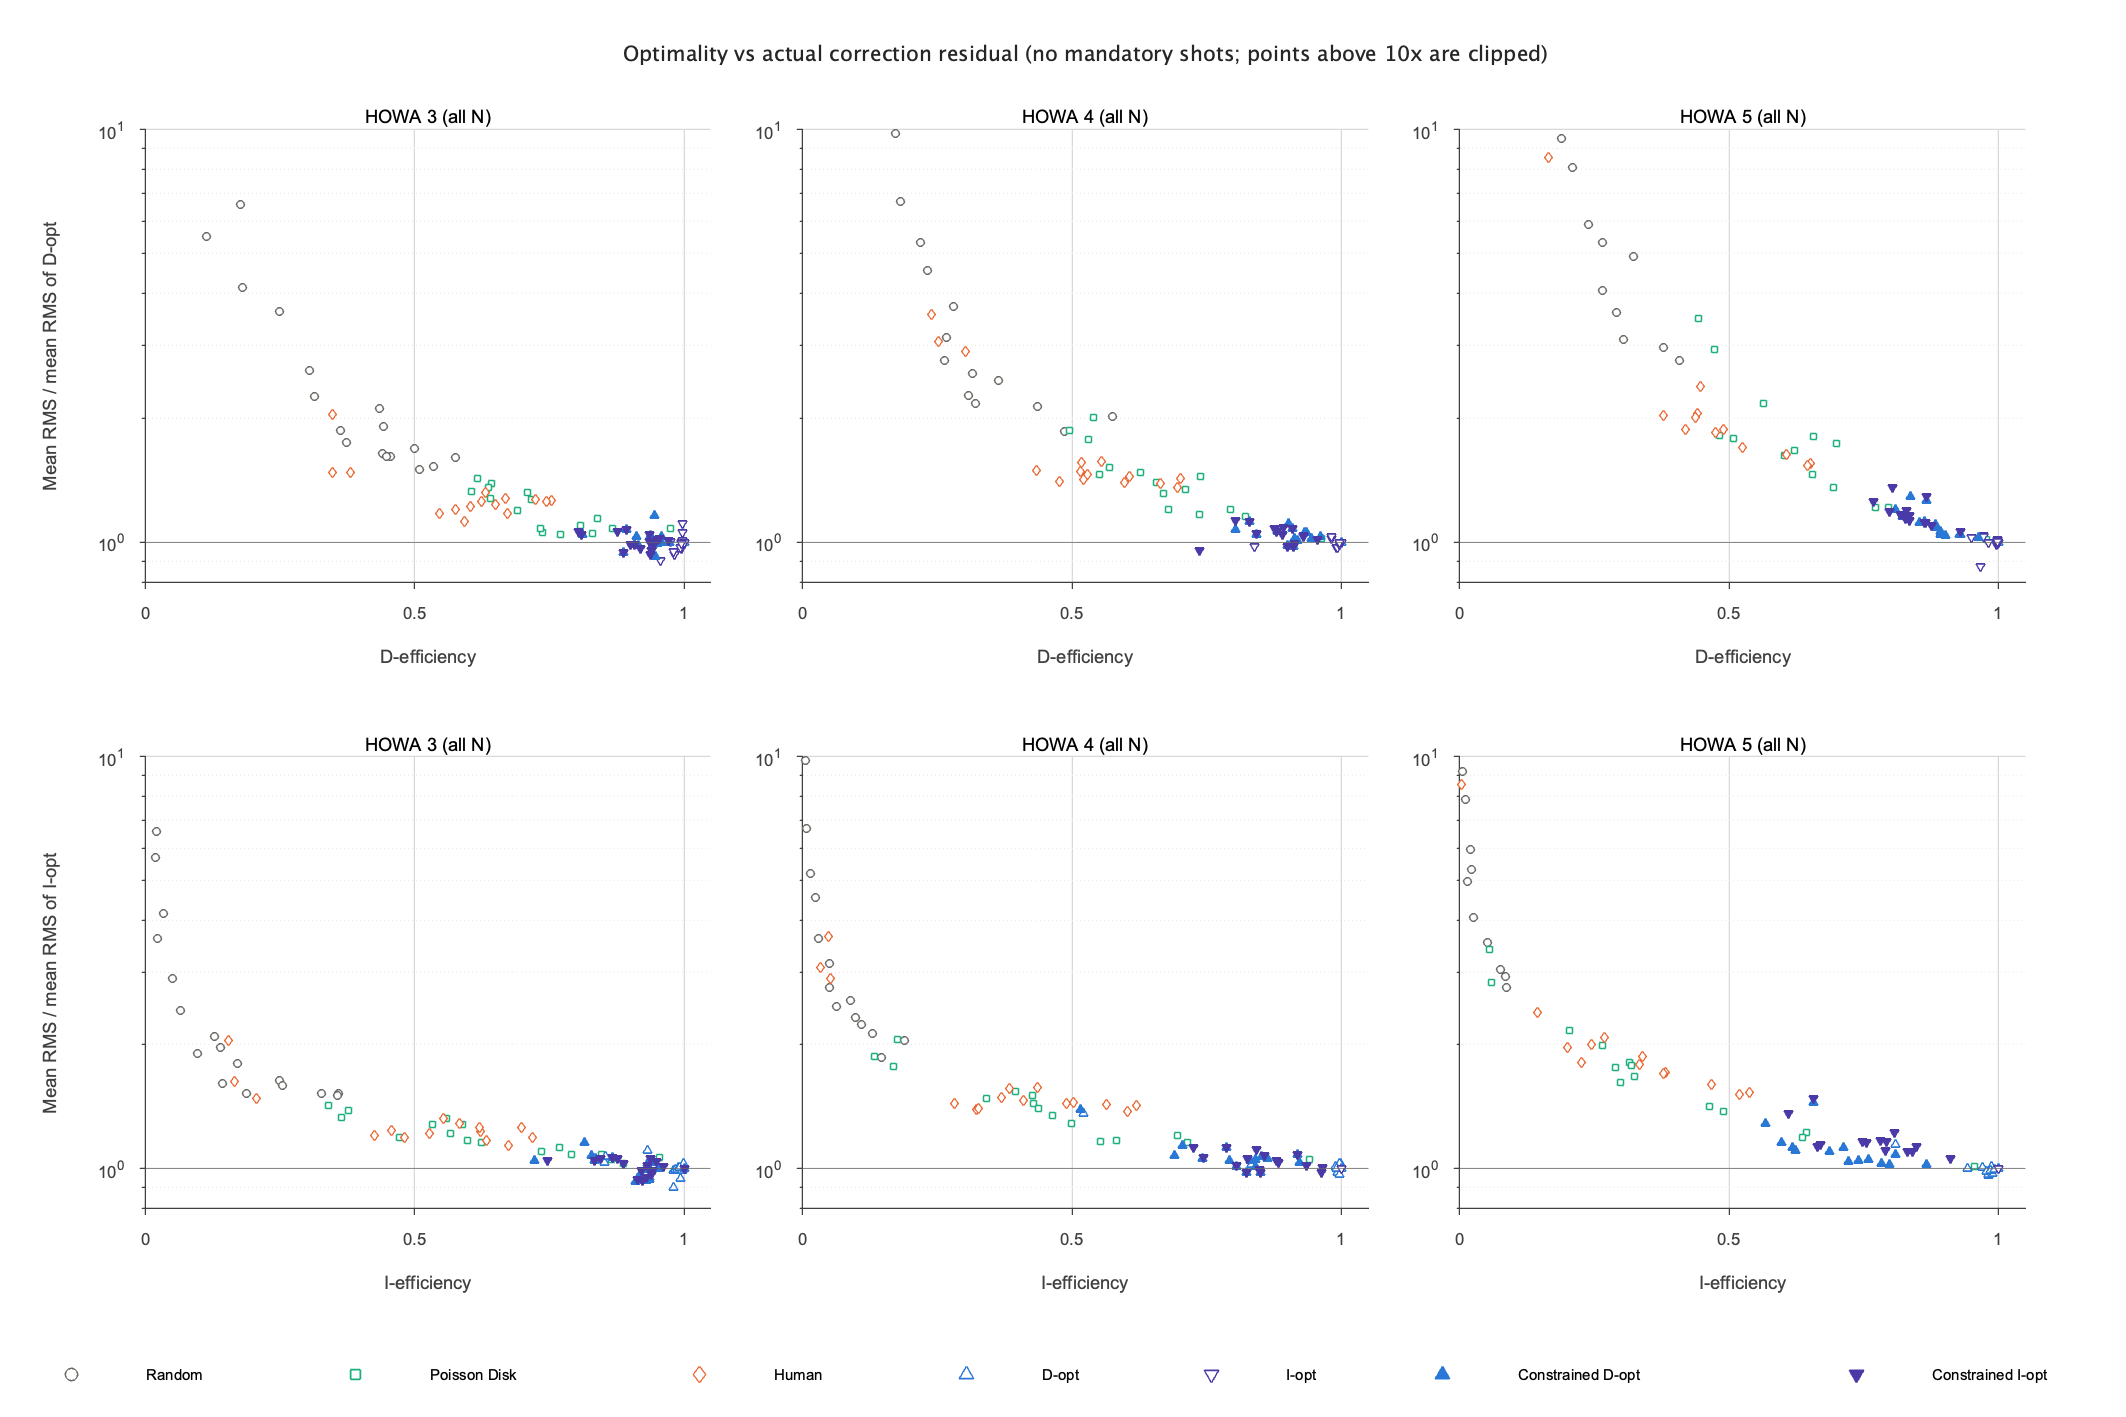
\includegraphics[width=\figw]{fig11_tradeoff_efficiency_vs_rms.png}
  \caption{D-efficiency（上）・I-efficiency（下）と，同じ$N$の制約なし最適に対する平均RMSの比（全$N$の設計）．}
  \label{fig:tradeoff}
\end{figure}

\subsection{実務制約による性能低下}

全評価点の平均RMSでみた性能低下は，$N=8$〜19の中央値で3次ほぼ0\%，4次約4\%，5次約8\%（C-D-opt）で，5次の$N=8$では約13\%に達した．
効率でみると，5次でD-efficiencyが約0.88，I-efficiencyが約0.72である．
性能低下の主因は半径領域制約（特にOuterの上限とInnerの下限）である．
高次モデル・少ないshot数で残差を優先する場合は，半径領域の目標割合を外周寄りにする，Innerの下限を1 shotに緩める，soft制約で小さな罰則にする，などの調整が考えられる．
これらはすべて設定ファイルの変更で評価できる．

\subsection{mandatory shotを考慮する意義}

強制計測shotの情報量を考慮しない素朴な方法は，追加shotが少ないとrank不足（推定不能）になった．推定できた場合も，拡張計画の残差は素朴な方法より最大71\%小さかった．
拡張計画は全shot数で推定可能で，追加shotが少ないほど効果が大きい．
一方，強制shotそのものが外周を測る余地を奪うため，強制shotの位置と数は残差に大きく影響する（5次$N=9$で強制shotなしの3倍）．
強制shotを決める工程側でも，本手法で「その強制shotを入れたときに残差がどれだけ増えるか」を見積もってから決めることが望ましい．

\subsection{実工程適用可能性}

設計は真値に依存しないので，shot配置・mark配置・制約・次数ごとに一度計算すればよい．
計算時間は1設計あたり平均0.1〜2秒程度（\ref{sec:time}節）で，レシピ作成時の計算として十分に短い．
制約は整数の上下限で表すため，工程ごとの要求（象限ごとの最低数，強制shot，scan方向）を設定ファイルで変えられる．
適用の前に，実データで次を確認する必要がある．
(1)実際のwafer変形の高次成分の大きさと形（モデル不一致の大きさ），(2)scan方向依存成分の大きさ（制約付き設計が有利になるかを左右する），(3)mark計測誤差，(4)partial shot領域の製品dieの重要度（外周を重視するか内側を重視するか）．

\subsection{限界と今後の課題}

\begin{itemize}
  \item 真値・scan成分・計測誤差はすべて仮定値に基づく模擬データであり，結論の大きさ（何\%良い・悪い）はこれらに依存する．特にscan方向依存成分の大きさで，制約付き設計の有利・不利が入れ替わる．
  \item 真値は動径次数7までのFringe Zernikeで，局所的な変形（edge rolloffなど）は含まない．局所変形があると，空間的に分散した設計の価値は高まると考えられる．
  \item 評価点はpartial shotのmarkを含む全有効markとした．評価の重みを製品dieの分布に合わせると結論が変わりうる（\ref{sec:tail}節）．
  \item 交換法は発見的手法で，制約付き設計では初期解の数\%しか最良値に達していない．multi-start 200回で20回より改善したが，大域最適の保証はない．
  \item shot単位の選択に限定し，mark単位の選択，markの計測失敗（欠測）への頑健性，shot内（intra-field）補正，複数layer・lot間の動的samplingは扱っていない．
  \item 今後は，実データでの検証，モデル不一致に頑健な設計（ベイズ最適計画など），製品die分布で重み付けしたI最適，欠測に頑健な設計，scan方向依存成分を明示的にモデルへ入れた設計を検討する．
\end{itemize}

% ============================================================
\section{まとめ}
% ============================================================

wafer高次補正（HOWA型3〜5次）のalignment計測shot選択について，象限・半径領域・scan方向・強制計測shot・partial shot除外の実務制約を整数の上下限として統合したD/I最適計画と，強制shotに対するoptimal augmentationを構築し，1000枚の模擬waferで補正後の残差を評価した．
結果を表\ref{tab:conclusion}にまとめる．

\begin{table}[htbp]
  \centering
  \caption{どの方式がどの条件で有利か（主評価条件，全評価点の平均RMSを基本とした判断）}
  \label{tab:conclusion}
  \small
  \begin{tabular}{p{30mm}p{125mm}}
    \toprule
    観点 & 結論 \\
    \midrule
    実務制約の適合性 & 制約を必ず満たすのは制約付き設計（C-D-opt・C-I-opt・Augmentation）だけ．制約なしD/I最適は半径領域制約をほぼ全設計で外れ，Random・Human・Poissonもscan方向制約を6〜8割の設計で外れた． \\
    Residual RMS（平均） & 制約を満たす方式の中では制約付きD/I最適が最良で，Humanより20〜39\%，Poissonより19〜35\%小さい（$N=8$〜19の中央値）．制約を問わなければ制約なしD/I最適が最良で，制約付きとの差は3次でほぼ0，4次で約4\%，5次で約8〜15\%． \\
    tail（P95・P99・Max） & waferごとのRMSのP95は平均と同じ順位．wafer内の最大残差は外周（partial shot領域）の外挿で決まり，制約なしD/I最適が有利．wafer内側だけなら制約付き設計の方が小さい． \\
    measurement shot数 & Humanの12 shot・19 shotと同じ平均RMSを，制約付き設計は6〜8 shot・7〜10 shotで達成（33〜63\%削減）． \\
    D-opt と I-opt & 制約なしではほぼ同じ設計・同じ残差．制約付きの5次ではC-D-optの方がC-I-optより残差が小さい場合が多かった．どちらか一方で十分で，迷えば制約付きD-optを推奨する． \\
    強制計測shot & 強制shotの情報量を考慮する拡張計画（Augmentation）を使う．素朴な方法は追加shotが少ないとrank不足になり，推定できても拡張計画の方が最大71\%小さい．$N\ge13$では差は小さい． \\
    scan方向依存成分 & 成分が大きいほど制約付き設計が有利（3次$N=12$で名目の4倍のとき23\%改善）．scan方向の均等化は最適性の損失がごく小さく，常に課してよい． \\
    \bottomrule
  \end{tabular}
\end{table}

結論として，D/I最適計画そのものの最適性は制約により数\%〜十数\%下がるが，実務制約を満たす配置の中では，提案手法（制約付きD/I最適，強制shotありでは拡張計画）がHuman・Poisson・Randomより明確に小さい補正残差を与え，同じ残差に必要な計測shot数を3〜6割減らせる．
制約の代償は高次・少shotほど大きく，その主因は半径領域制約による外周shotの不足であるため，次数とshot数に応じて半径領域の目標割合を調整することを推奨する．

% ============================================================
\section*{謝辞}
\addcontentsline{toc}{section}{謝辞}
% ============================================================

% ← 謝辞を記入する（以下は仮の文面）
本検討にあたり議論いただいた関係各位に感謝する．

% ============================================================
\addcontentsline{toc}{section}{参考文献}
\begin{thebibliography}{99}
\small
\bibitem{slonaker1988} S. Slonaker, S. McNamara, K. Konno, et al.，``Enhanced global alignment for production optical lithography,'' Proc. SPIE 922 (Optical/Laser Microlithography), 73-81（1988）． doi:\href{https://doi.org/10.1117/12.968404}{10.1117/12.968404}．
\bibitem{adel2007} M. Adel, P. Izikson, D. Tien, et al.，``The challenges of transitioning from linear to high-order overlay control in advanced lithography,'' Proc. SPIE 6827, 682722（2007）． doi:\href{https://doi.org/10.1117/12.778457}{10.1117/12.778457}．
\bibitem{us9291916} S. C. T. Van Der Sanden, R. J. F. Van Haren, H. J. G. Simons, et al.（ASML Netherlands B.V.），``Method of applying a pattern to a substrate, device manufacturing method and lithographic apparatus for use in such methods,'' US9291916B2（2016）． \url{https://patents.google.com/patent/US9291916B2/en}．
\bibitem{wang2009} R. Wang, C. Chiang, W. Hsu, et al.，``Overlay improvement by ASML HOWA 5th alignment strategy,'' Proc. SPIE 7520 (Lithography Asia 2009), 752023（2009）． doi:\href{https://doi.org/10.1117/12.839816}{10.1117/12.839816}．
\bibitem{pike2012} M. Pike, N. Felix, V. Menon, et al.，``High-order wafer alignment in manufacturing,'' Proc. SPIE 8324, 832408（2012）． doi:\href{https://doi.org/10.1117/12.916483}{10.1117/12.916483}．
\bibitem{jeon2013} B. Jeon, S. Pal, S. Mehta, et al.，``High order wafer alignment for 20nm node logic process,'' Proc. SPIE 8681, 868110（2013）． doi:\href{https://doi.org/10.1117/12.2010709}{10.1117/12.2010709}．
\bibitem{chiu2012} C. Chiu, C. Huang, J. Shieh, et al.，``Impacts of overlay correction model and metrology sampling scheme on device yield,'' Proc. SPIE 8324, 83241S（2012）． doi:\href{https://doi.org/10.1117/12.916601}{10.1117/12.916601}．
\bibitem{canon_ms001} C. Inc.，``New Canon wafer measurement equipment improves productivity of lithography systems, enabling high-precision alignment for increasingly complex semiconductor manufacturing processes,'' Web page（2023，2026-10-04 閲覧）． \url{https://global.canon/en/news/2023/20230221.html}．
\bibitem{nikon_litho_booster} N. P. Inc.，``Litho Booster Standalone Alignment Station,'' Web page（2026，2026-10-04 閲覧）． \url{https://www.nikonprecision.com/products-and-technology/alignment-stations/litho-booster/}．
\bibitem{us5493402} （Nikon Corporation），``EGA alignment method using a plurality of weighting coefficients,'' US5493402A（1996）． \url{https://patents.google.com/patent/US5493402A/en}．
\bibitem{chiu2022a} C. Chiu, F. Tian, W. Feng, et al.，``A comprehensive study of scanner alignment mark quantity and layout-dependent effect for overlay performance optimization,'' Proc. SPIE 12053, 1205319（2022）． doi:\href{https://doi.org/10.1117/12.2614375}{10.1117/12.2614375}．
\bibitem{chue2009} C. Chue, T. Chiou, C. Huang, et al.，``Optimization of alignment/overlay sampling and marker layout to improve overlay performance for double patterning technology,'' Proc. SPIE 7520 (Lithography Asia 2009), 75200G（2009）． doi:\href{https://doi.org/10.1117/12.837137}{10.1117/12.837137}．
\bibitem{us20160334717} J. S. Wildenberg, E. C. Mos（ASML），``Method of determining a measurement subset of metrology points on a substrate, associated apparatus and computer program,'' US20160334717A1（2016）． \url{https://patents.google.com/patent/US20160334717A1/en}．
\bibitem{us20160299438} E. C. Mos, E. M. M. Crombag, A. Ganesan（ASML），``Method and apparatus for inspection and metrology,'' US20160299438A1（2016）． \url{https://patents.google.com/patent/US20160299438A1/en}．
\bibitem{wo2020234028} P. G. J. Smorenberg, P. Saputra, K. Elbattay, et al.（ASML Netherlands B.V.），``Method for determining a sampling scheme, a semiconductor substrate measurement apparatus, a lithographic apparatus,'' WO2020234028A1（2020）． \url{https://patents.google.com/patent/WO2020234028A1/en}．
\bibitem{us11775728} P. Frisco（ASML Netherlands B.V.），``Methods for sample scheme generation and optimization,'' US11775728B2（2023）． \url{https://patents.google.com/patent/US11775728B2/en}．
\bibitem{us7042552} R. Werkman, F. B. M. Van Bilsen, B. Swinnen（ASML Netherlands B.V.），``Alignment strategy optimization method,'' US7042552B1（2006）． \url{https://patents.google.com/patent/US7042552B1/en}．
\bibitem{us7197722} A. Wong, J. Drautz, J. D. Shindler, et al.（Intel Corporation），``Optimization of sample plan for overlay,'' US7197722B2（2007）． \url{https://patents.google.com/patent/US7197722B2/en}．
\bibitem{us7571420} A. Wong, J. Drautz, J. D. Shindler, et al.（Intel Corporation），``Dynamic sampling with efficient model for overlay,'' US7571420B2（2009）． \url{https://patents.google.com/patent/US7571420B2/en}．
\bibitem{us10692227} B. A. Riggs, O. N. Demirer, W. Pierson（KLA），``Determination of sampling maps for alignment measurements based on reduction of out of specification points,'' US10692227B2（2020）． \url{https://patents.google.com/patent/US10692227B2/en}．
\bibitem{koay2010} C. Koay, M. E. Colburn, P. Izikson, et al.，``Automated optimized overlay sampling for high-order processing in double patterning lithography,'' Proc. SPIE 7638, 76381R（2010）． doi:\href{https://doi.org/10.1117/12.846371}{10.1117/12.846371}．
\bibitem{us4918320} B. Hamasaki, H. Igarashi, A. Nakai, et al.（Canon），``Alignment method usable in a step-and-repeat type exposure apparatus for either global or dye-by-dye alignment,'' US4918320A（1990）． \url{https://patents.google.com/patent/US4918320A/en}．
\bibitem{us12025924} S. Egashira（Canon），``Method of determining set of sample shot regions, method of obtaining measurement value, information processing apparatus, lithography apparatus, storage medium, and article manufacturing method,'' US12025924B2（2024）． \url{https://patents.google.com/patent/US12025924B2/en}．
\bibitem{jph1019512} K. Hizuka（Nikon），``Positioning method,'' JPH1019512A（1998）． \url{https://patents.google.com/patent/JPH1019512A/en}．
\bibitem{felix2011} N. M. Felix, A. H. Gabor, V. C. Menon, et al.，``Overlay improvement roadmap: Strategies for scanner control and product disposition for 5-nm overlay,'' （2011）． doi:\href{https://doi.org/10.1117/12.879532}{10.1117/12.879532}．
\bibitem{lee2016} H. Lee, S. Han, M. Kim, et al.，``In-depth analysis of sampling optimization methods,'' （2016）． doi:\href{https://doi.org/10.1117/12.2219037}{10.1117/12.2219037}．
\bibitem{chiu2022b} C. Chiu, F. Tian, W. Feng, et al.，``A new development algorithm to optimize scanner alignment sampling for cross-chuck overlay performance optimization,'' Proc. SPIE 12053（2022）． doi:\href{https://doi.org/10.1117/12.2627283}{10.1117/12.2627283}．
\bibitem{fedorov1972} V. V. Fedorov，\textit{Theory of Optimal Experiments}，Academic Press（1972）．
\bibitem{atkinson2007} A. C. Atkinson, A. N. Donev, R. D. Tobias，\textit{Optimum Experimental Designs, with SAS}，Oxford University Press（2007）．
\bibitem{goos2011} P. Goos, B. Jones，\textit{Optimal Design of Experiments: A Case Study Approach}，Wiley（2011）．
\bibitem{jones2012} B. Jones, P. Goos，``I-optimal versus D-optimal split-plot response surface designs,'' Journal of Quality Technology 44(2), 85-101（2012）． doi:\href{https://doi.org/10.1080/00224065.2012.11917886}{10.1080/00224065.2012.11917886}．
\bibitem{mitchell1974} T. J. Mitchell，``An algorithm for the construction of "D-optimal" experimental designs,'' Technometrics 16(2), 203-210（1974）． doi:\href{https://doi.org/10.1080/00401706.1974.10489175}{10.1080/00401706.1974.10489175}．
\bibitem{cook1980} R. D. Cook, C. J. Nachtsheim，``A comparison of algorithms for constructing exact D-optimal designs,'' Technometrics 22(3), 315-324（1980）． doi:\href{https://doi.org/10.1080/00401706.1980.10486162}{10.1080/00401706.1980.10486162}．
\bibitem{meyer1995} R. K. Meyer, C. J. Nachtsheim，``The coordinate-exchange algorithm for constructing exact optimal experimental designs,'' Technometrics 37(1), 60-69（1995）． doi:\href{https://doi.org/10.1080/00401706.1995.10485889}{10.1080/00401706.1995.10485889}．
\bibitem{dykstra1971} O. Dykstra，``The augmentation of experimental data to maximize |X'X|,'' Technometrics 13(3), 682-688（1971）． doi:\href{https://doi.org/10.1080/00401706.1971.10488830}{10.1080/00401706.1971.10488830}．
\bibitem{bridson2007} R. Bridson，``Fast Poisson disk sampling in arbitrary dimensions,'' ACM SIGGRAPH 2007 Sketches, 22（2007）． doi:\href{https://doi.org/10.1145/1278780.1278807}{10.1145/1278780.1278807}．
\bibitem{wyant1992} J. C. Wyant, K. Creath，``Basic wavefront aberration theory for optical metrology,'' in Applied Optics and Optical Engineering, Vol. XI (Academic Press)，pp.~1-53（1992）． \url{https://wp.optics.arizona.edu/jcwyant/wp-content/uploads/sites/13/2016/08/03-BasicAberrations_and_Optical_Testing.pdf}．
\bibitem{efron1993} B. Efron, R. J. Tibshirani，\textit{An Introduction to the Bootstrap}，Chapman \& Hall（1993）．
\end{thebibliography}


% ============================================================
\clearpage
\appendix
\section{代表wafer 3例}
\label{sec:appendix}
% ============================================================

代表waferは，恣意的にならないよう次のルールをコード（\texttt{select\_appendix\_samples}）で決めて選んだ．
対象は主評価条件・強制計測shotなし・HOWA 4次・$N=12$の7手法である．

\begin{description}
  \item[Sample 1（典型例）] 7手法の平均RMSが，1000 waferのその値の中央値に最も近いwafer．
  \item[Sample 2（改善が大きい例）] Constrained I-optの，Random・Poisson・Human・D-opt・I-optに対する平均改善率が，1000 waferの90\%点に最も近いwafer（最大値は外れ値になりやすいため分位点にした）．
  \item[Sample 3（難しい例）] 7手法の中で最も小さいRMSが最大のwafer（どの手法でも残差が大きい）．
\end{description}

\begin{table}[htbp]
  \centering
  \caption{代表wafer（HOWA 4次，$N=12$，主評価条件）．RMSは7手法の平均・最小と，C-I-optの比較手法に対する平均改善率}
  \label{tab:samples}
  \footnotesize
  \begin{tabular}{lrrrrrr}
    \toprule
    & wafer & 項数（X/Y） & 真値RMS（X/Y）[nm] & 下限 [nm] & 平均RMS [nm] & 最小RMS [nm] \\
    \midrule
    Sample 1（典型） & 732 & 19 / 17 & 2.22 / 2.59 & 0.50 & 1.32 & 0.99 \\
    Sample 2（改善大） & 910 & 10 / 10 & 1.48 / 1.00 & 0.49 & 1.40 & 0.91 \\
    Sample 3（難しい） & 724 & 19 / 10 & 2.58 / 1.00 & 0.97 & 2.09 & 1.49 \\
    \bottomrule
  \end{tabular}
\end{table}
「下限」はHOWA 4次で全評価点・誤差なしのときの残差（モデル不一致）．Sample 2・3のY成分は生成時のRMSが1\,nm未満だったため1\,nmへ拡大している．


各Sampleについて，(1)真のwafer面内傾向（X・Y成分の色マップと，ベクトル場・大きさ），(2)7手法のsampling map（背景はそのwaferの真の変位の大きさ），(3)HOWA 4次補正後の残差ベクトル場（背景は残差の大きさ）を示す．
(3)の色とベクトルの尺度は全手法で共通にした．ただし最大値に合わせると残差の大きい手法（主にRandom）で他が見えなくなるため，手法間の中央値で尺度を決め，それを超える色は飽和させ，矢印は20\,mmで切った（図中に明記）．
各図の上にはその手法の評価点（312点）でのRMS・P95・Maxを示した．これは表\ref{tab:tail}などと同じ定義の値である．
強制計測shotありの条件の図（☆が強制shot）も同じ形式で\texttt{results/figures/appendix/}に出力した（A.4節にSample 1の例を示す）．

\clearpage
\subsection{Sample 1}

\subsubsection*{真のwafer面内傾向}
\begin{figure}[H]
  \centering
  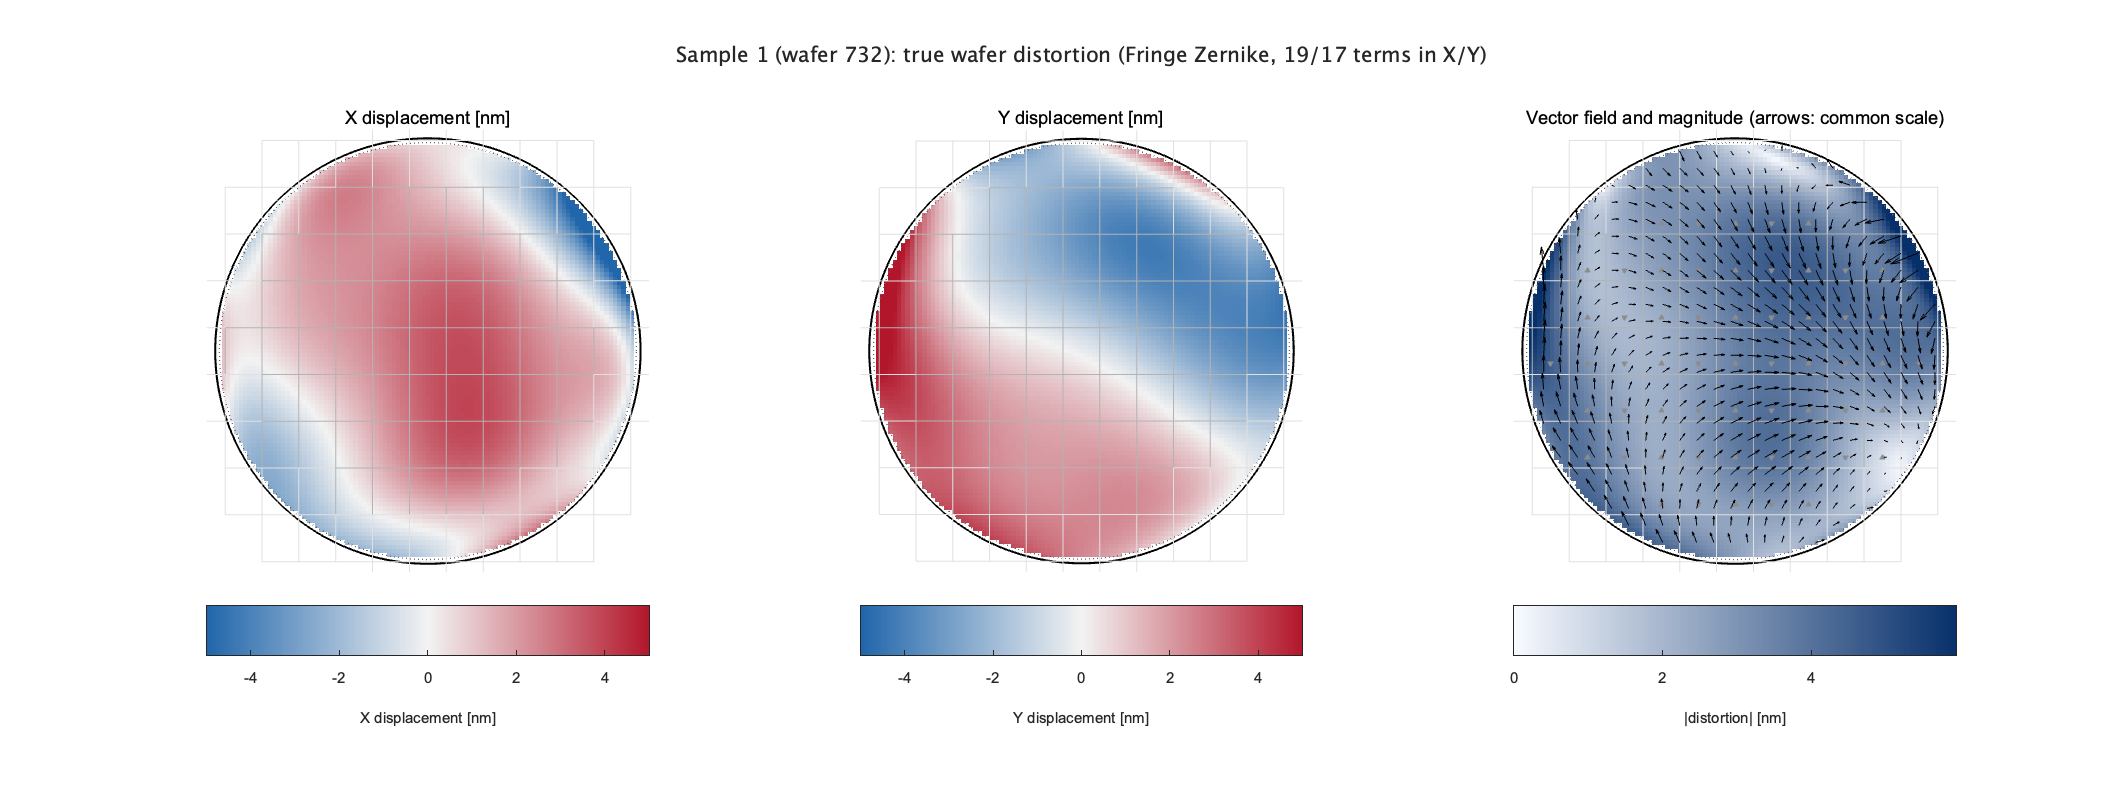
\includegraphics[width=0.92\textwidth]{A1_sample1_truth.png}
  \caption{Sample 1 の真の面内傾向．左・中：X・Y成分，右：ベクトル場と大きさ（▲▼はscan方向，格子はshot）．}
\end{figure}

\subsubsection*{sampling map}
\begin{figure}[H]
  \centering
  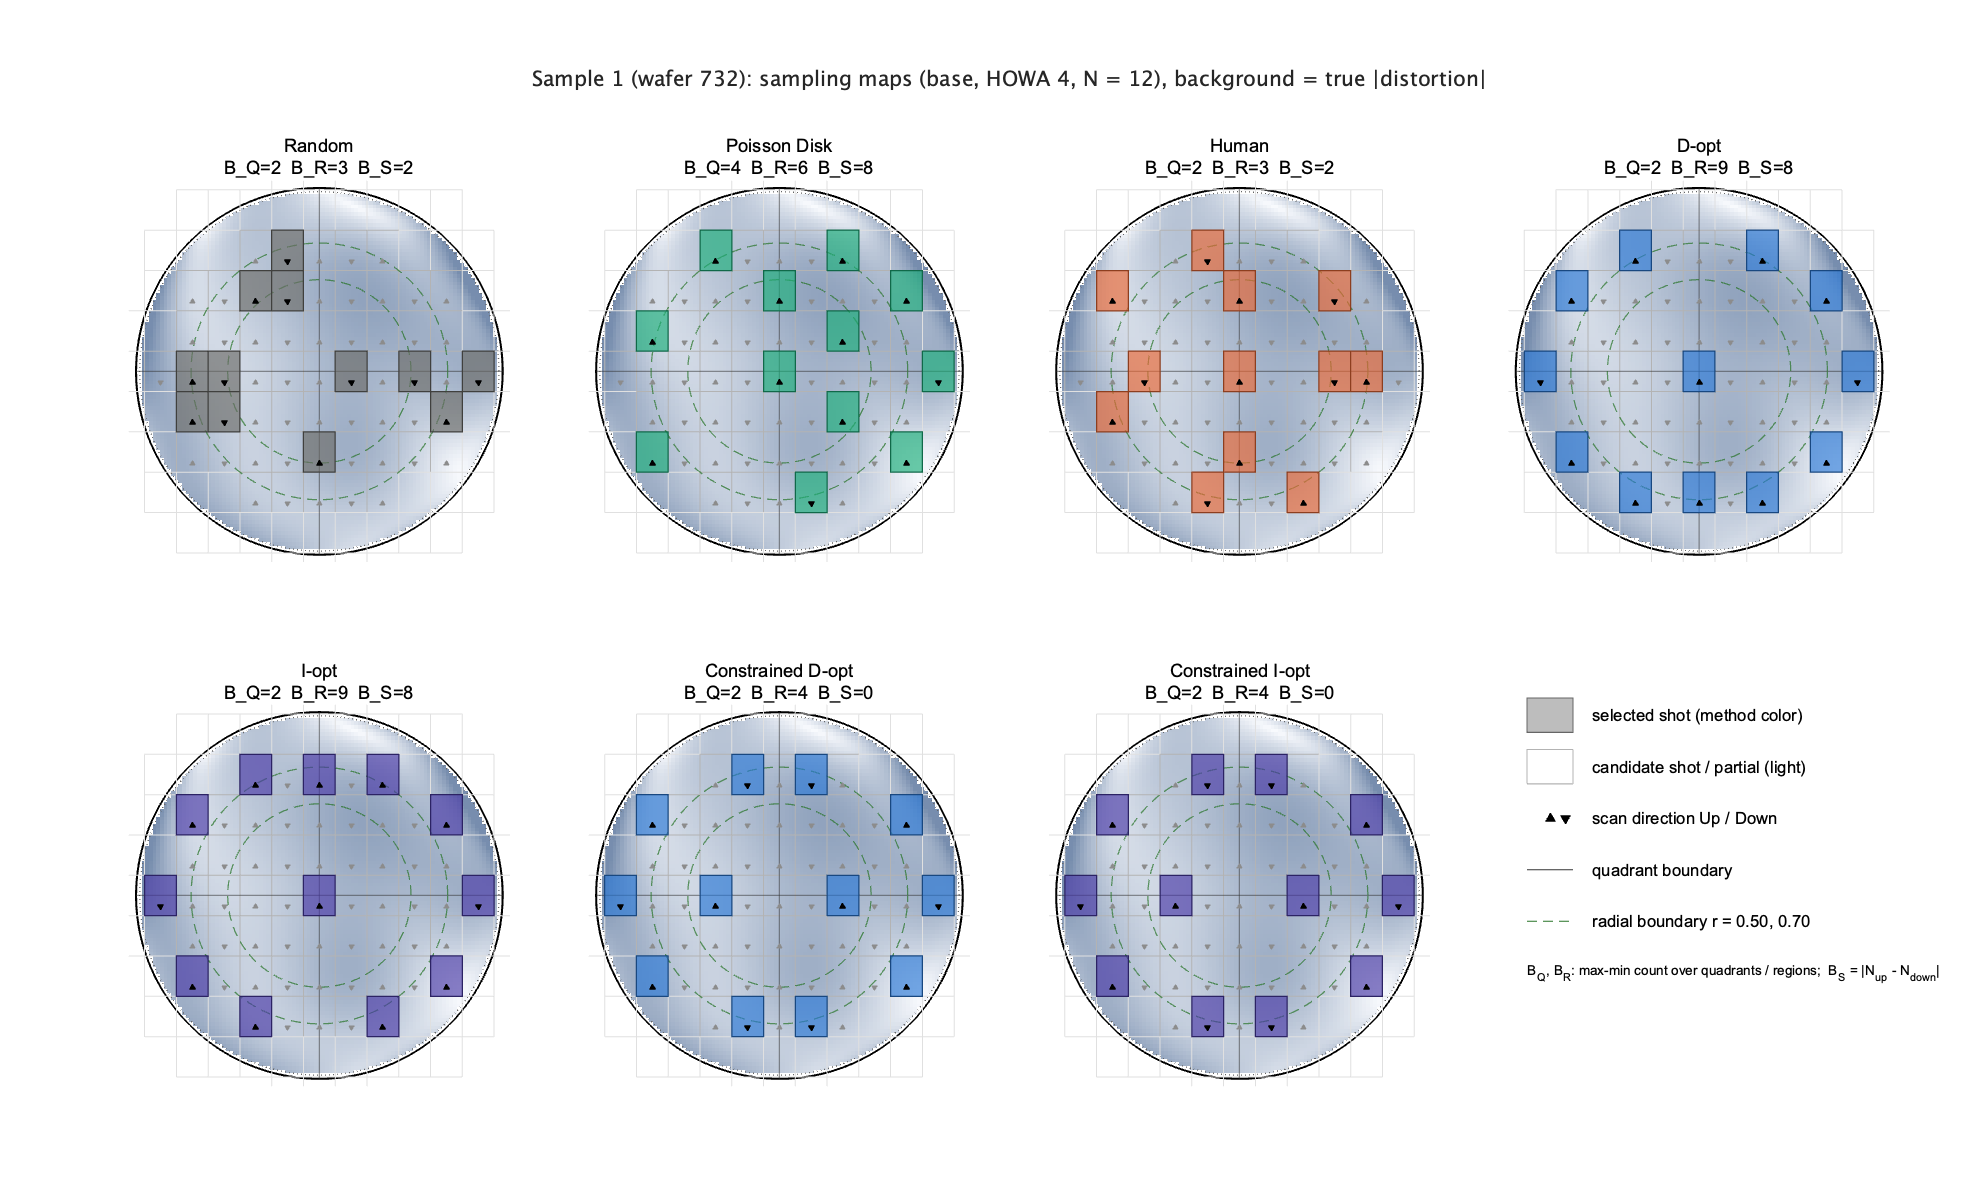
\includegraphics[width=0.85\textwidth]{A2_sample1_sampling_base.png}
  \caption{Sample 1 の sampling map（HOWA 4次，$N=12$）．背景はそのwaferの真の変位の大きさ．}
\end{figure}

\subsubsection*{補正後残差vector field}
\begin{figure}[H]
  \centering
  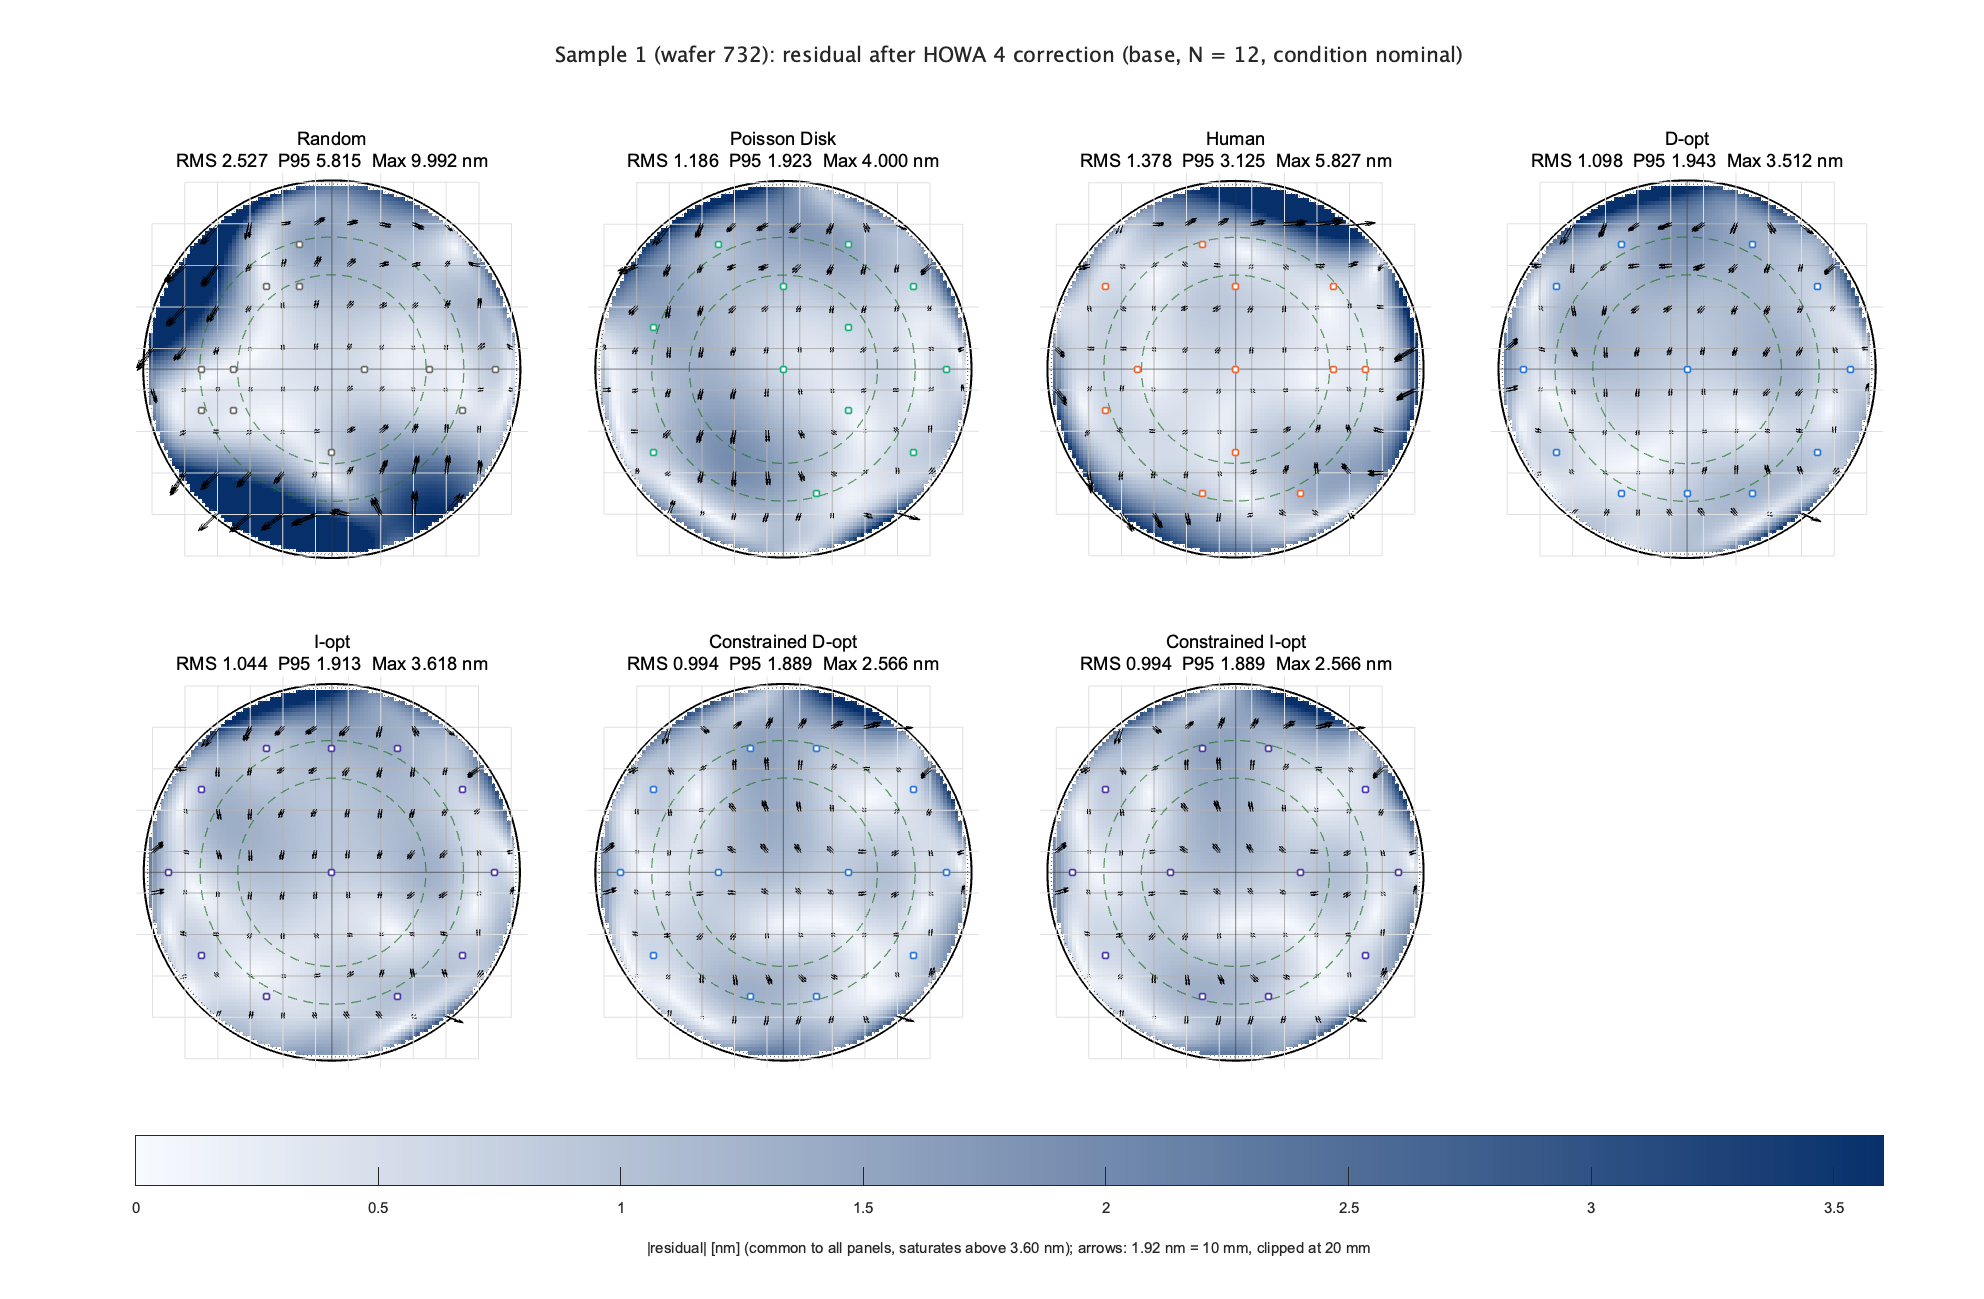
\includegraphics[width=0.85\textwidth]{A3_sample1_residual_base.png}
  \caption{Sample 1 のHOWA 4次補正後の残差（色と矢印の尺度は全手法で共通）．}
\end{figure}

Sample 1は平均的な難しさのwaferである．
補正後のRMSは，C-D-opt・C-I-opt（この条件では同じ設計）0.99\,nm，I-opt 1.04，D-opt 1.10，Poisson 1.19，Human 1.38，Random 2.53\,nmで，wafer内の最大残差もC-D-optが2.57\,nmとD-opt（3.51）より小さかった．
D-optでは外周とwafer中心の間（Inner〜Middle領域）に残差が広く残り，Inner・Middleにもshotを置いた制約付き設計ではその領域の残差が小さい．
Randomは測っていない左上と下側の外周で外挿が大きく外れている．


\clearpage
\subsection{Sample 2}

\subsubsection*{真のwafer面内傾向}
\begin{figure}[H]
  \centering
  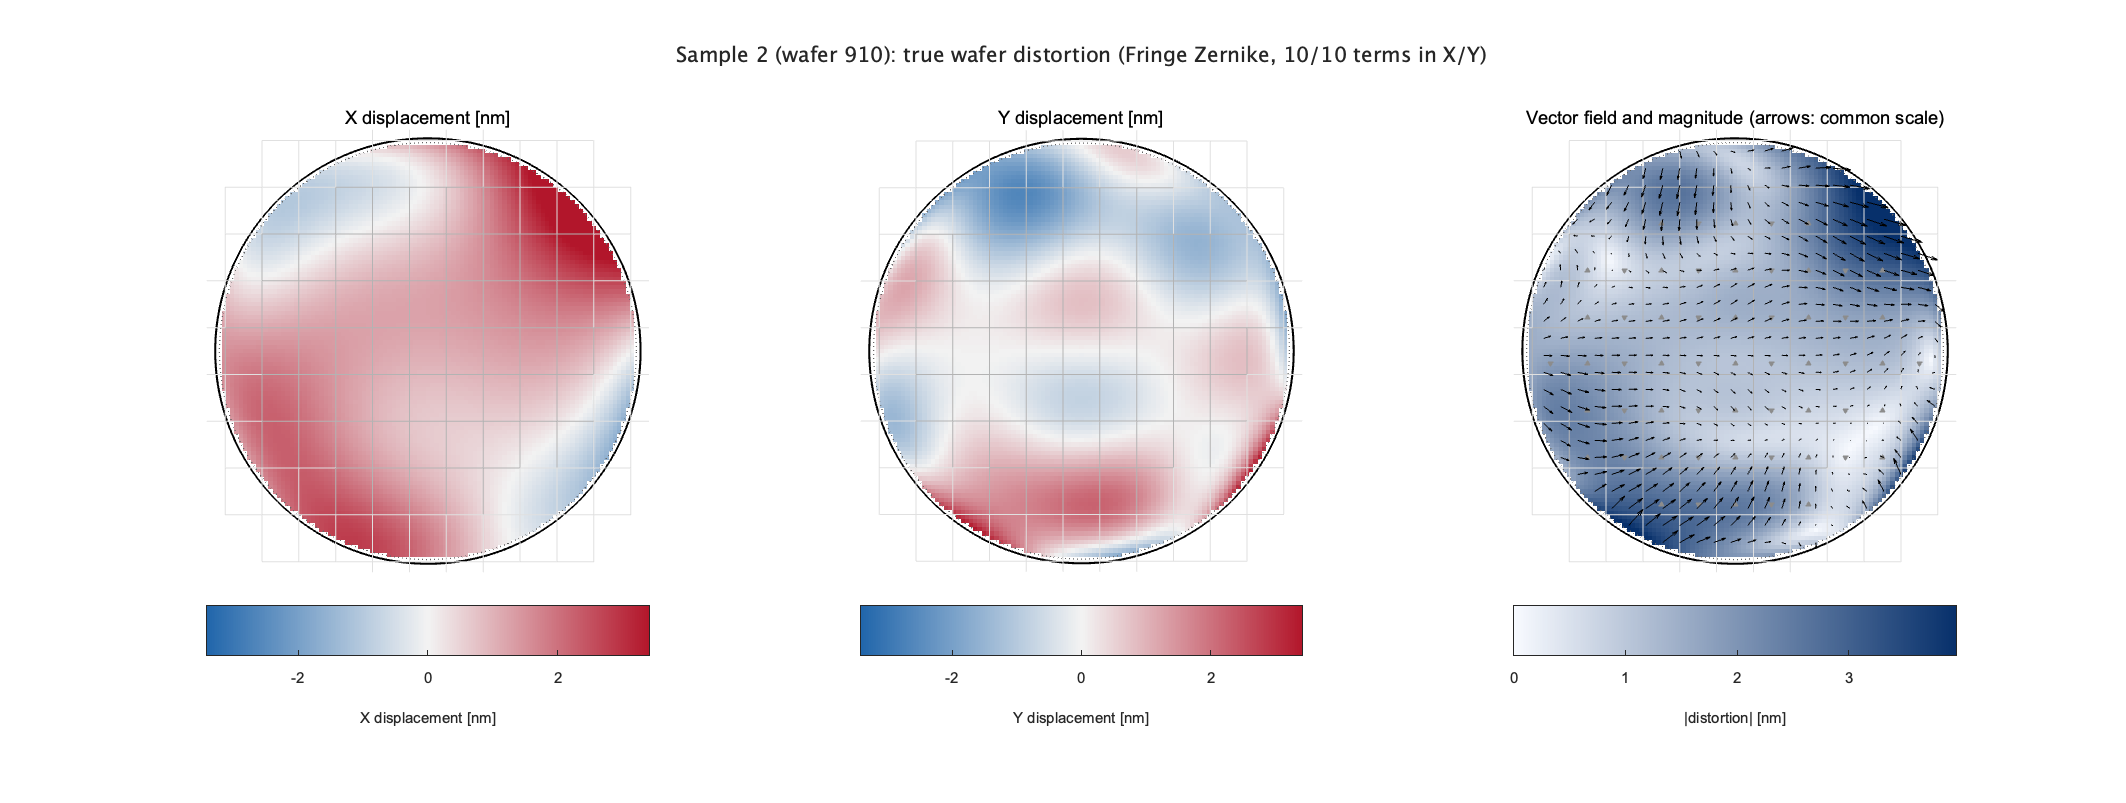
\includegraphics[width=0.92\textwidth]{A1_sample2_truth.png}
  \caption{Sample 2 の真の面内傾向．}
\end{figure}

\subsubsection*{sampling map}
\begin{figure}[H]
  \centering
  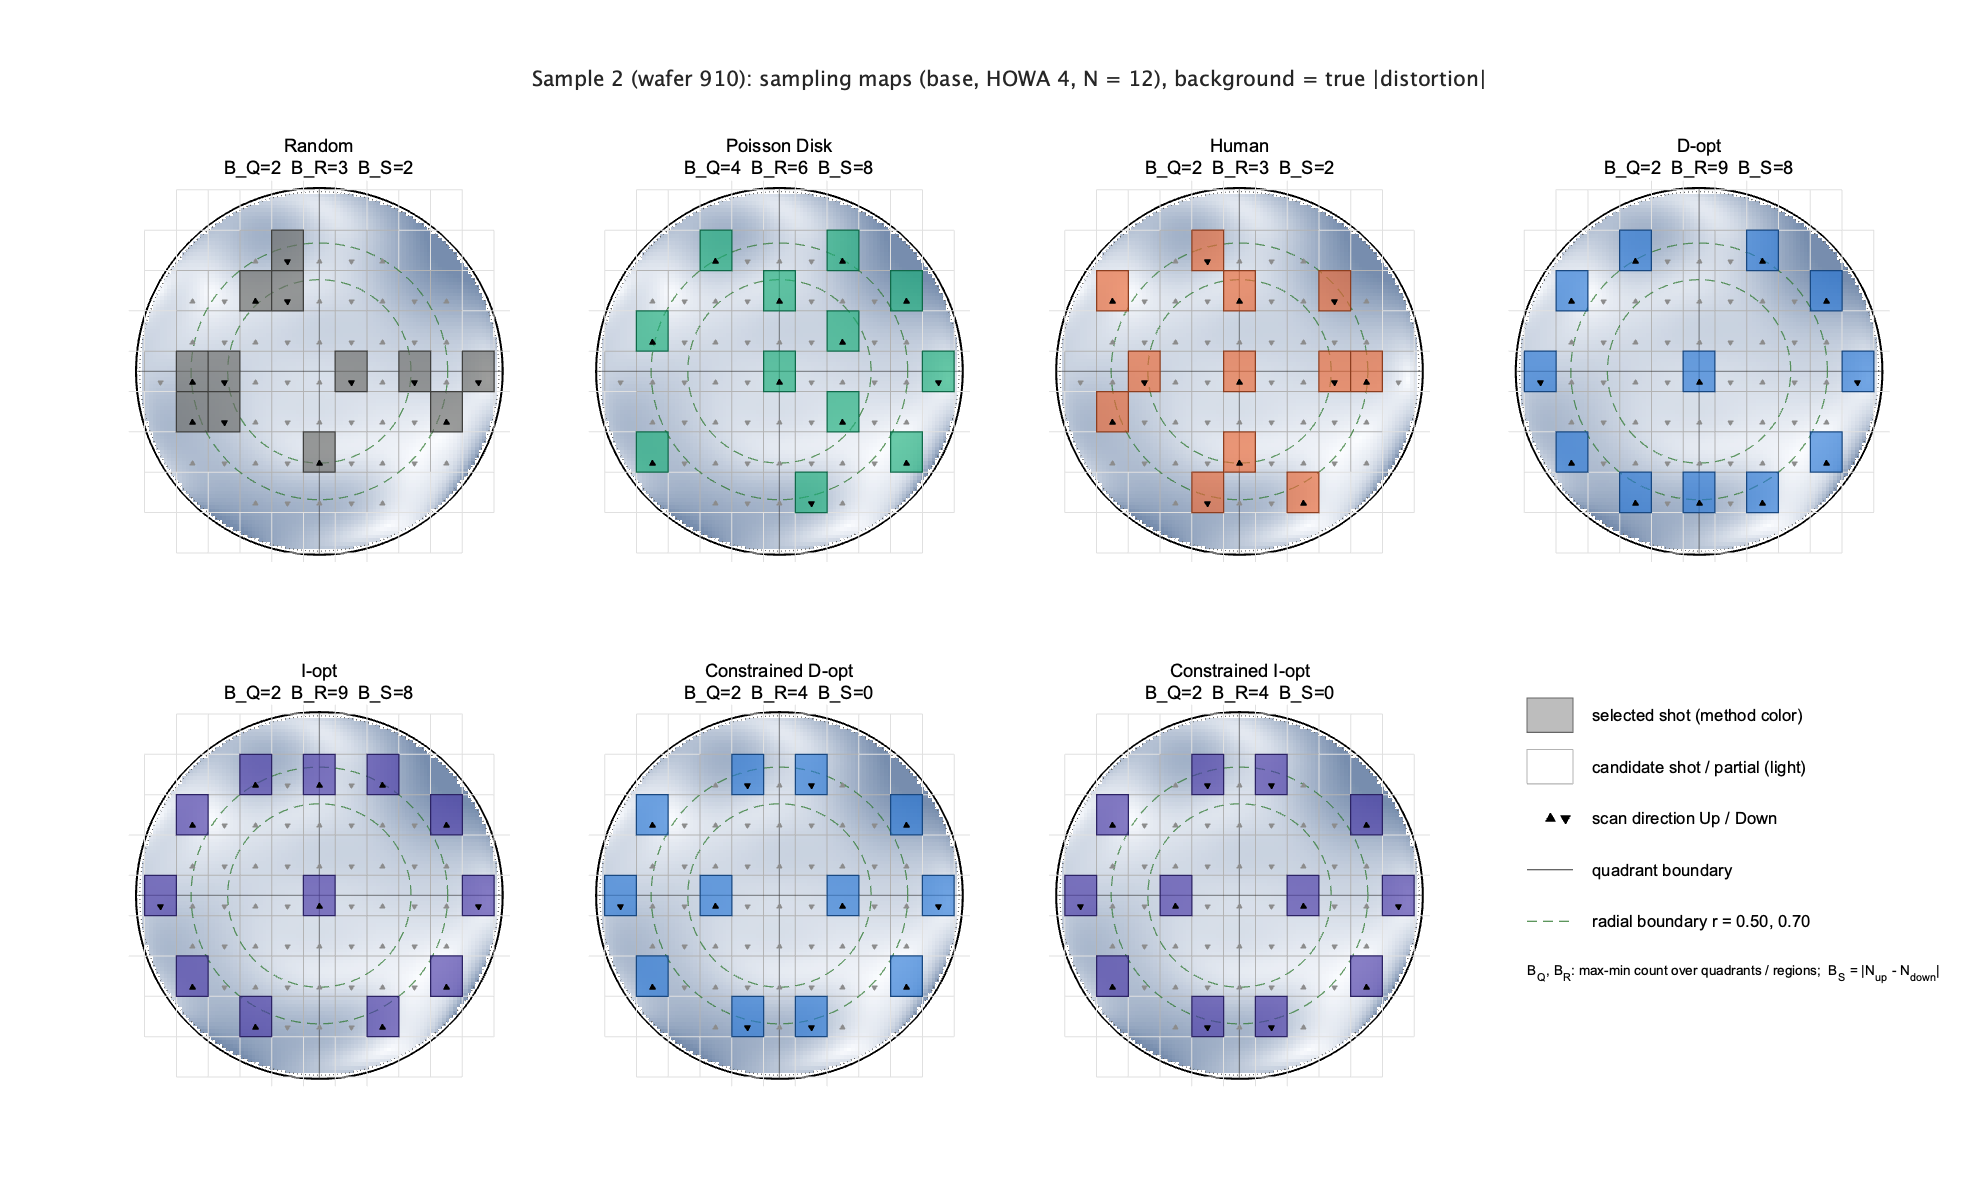
\includegraphics[width=0.85\textwidth]{A2_sample2_sampling_base.png}
  \caption{Sample 2 の sampling map（HOWA 4次，$N=12$）．}
\end{figure}

\subsubsection*{補正後残差vector field}
\begin{figure}[H]
  \centering
  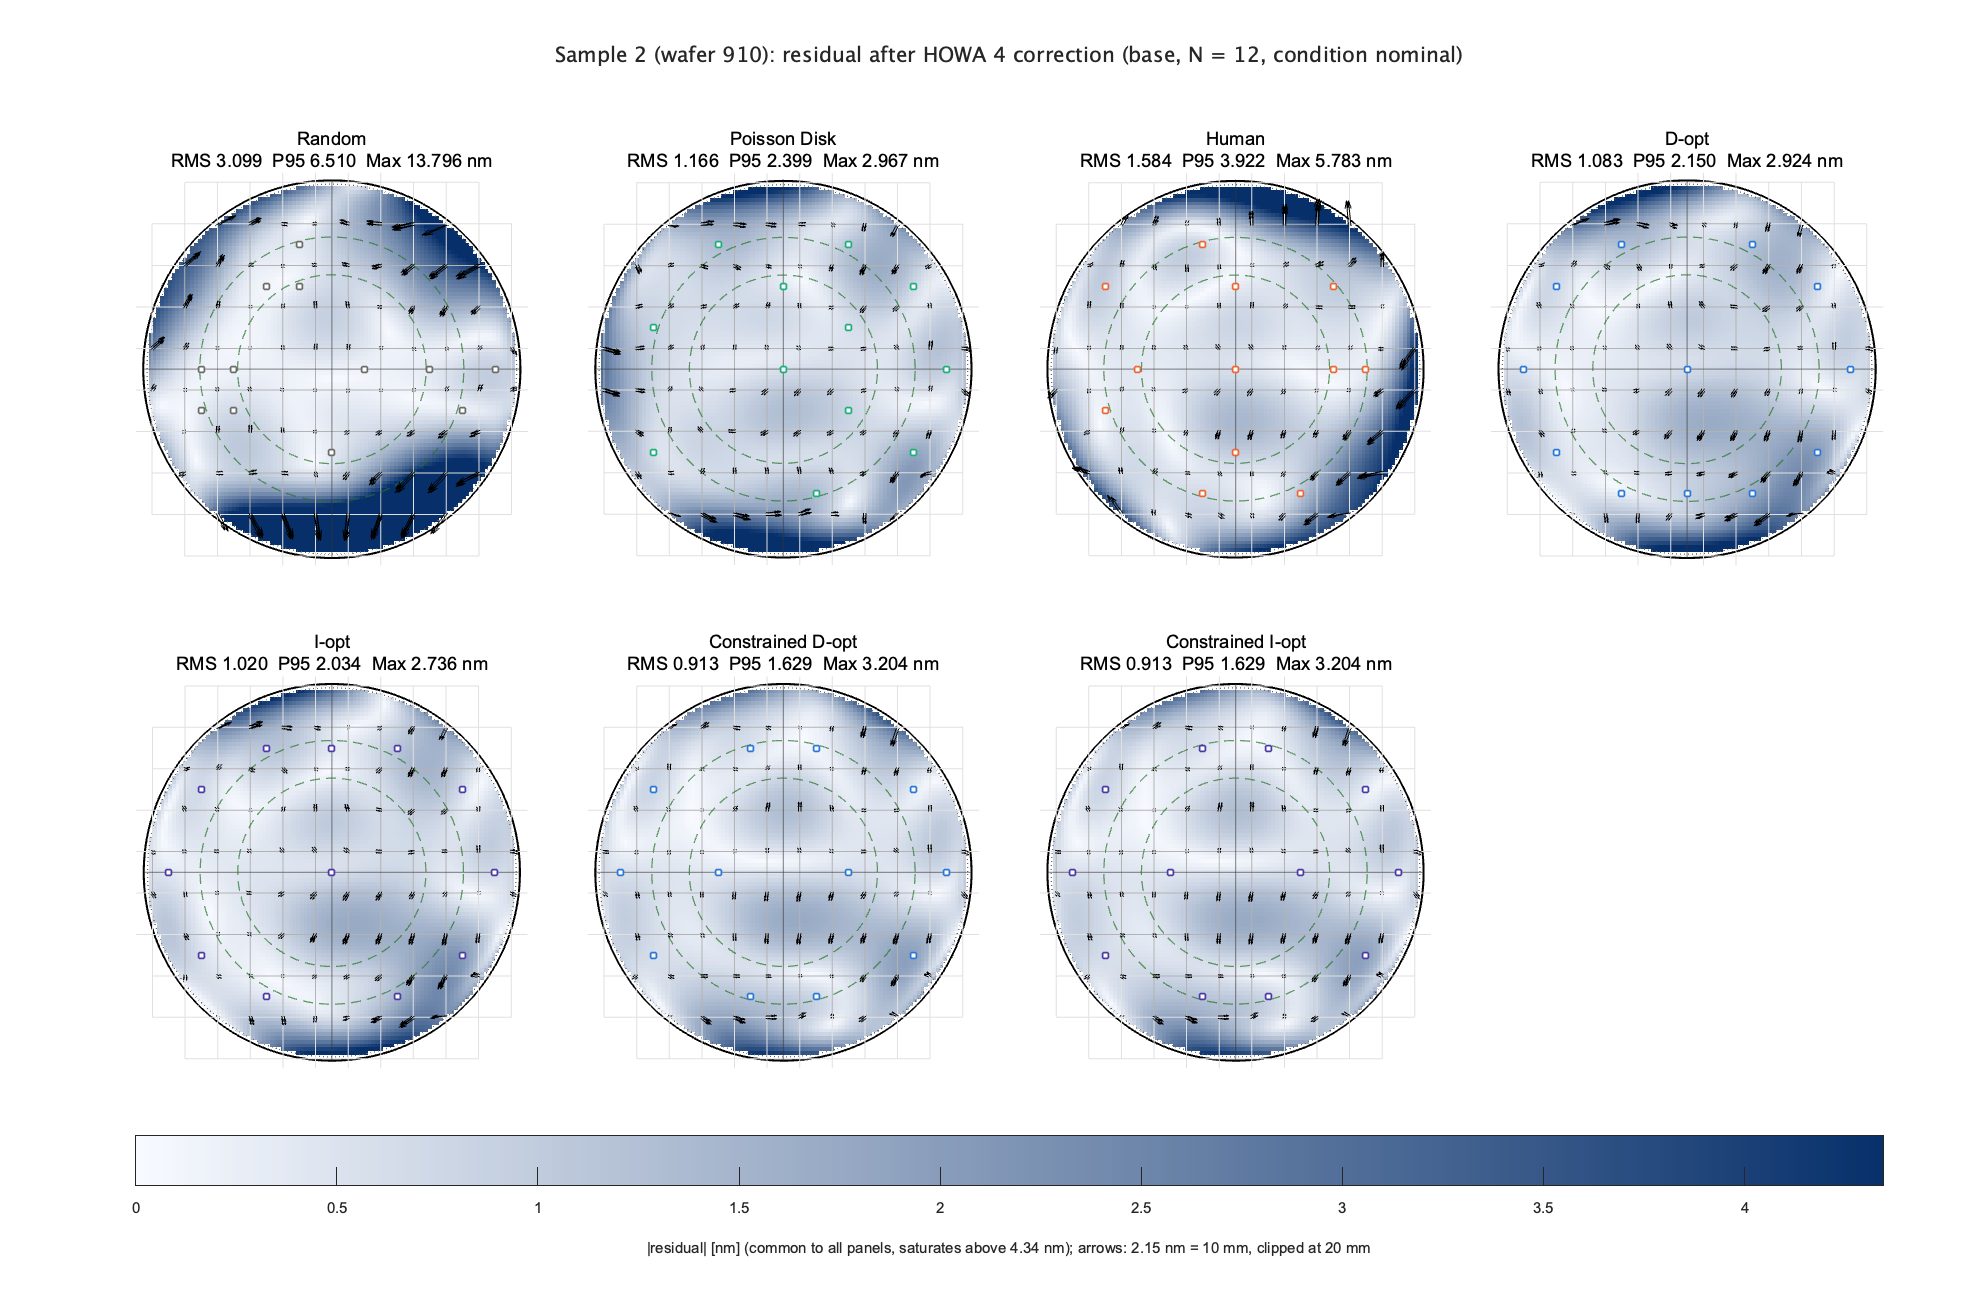
\includegraphics[width=0.85\textwidth]{A3_sample2_residual_base.png}
  \caption{Sample 2 のHOWA 4次補正後の残差．}
\end{figure}

Sample 2は提案法の改善が大きい例で，C-D-opt・C-I-optのRMSは0.91\,nm（D-opt 1.08，I-opt 1.02，Poisson 1.17，Human 1.58，Random 3.10）だった．
P95もC-D-optが1.63\,nmとD-opt（2.15）より小さい．一方，最大残差はC-D-opt 3.20\,nm，D-opt 2.92\,nmで，外周の外挿は制約なしの方が良い（\ref{sec:tail}節と同じ傾向）．


\clearpage
\subsection{Sample 3}

\subsubsection*{真のwafer面内傾向}
\begin{figure}[H]
  \centering
  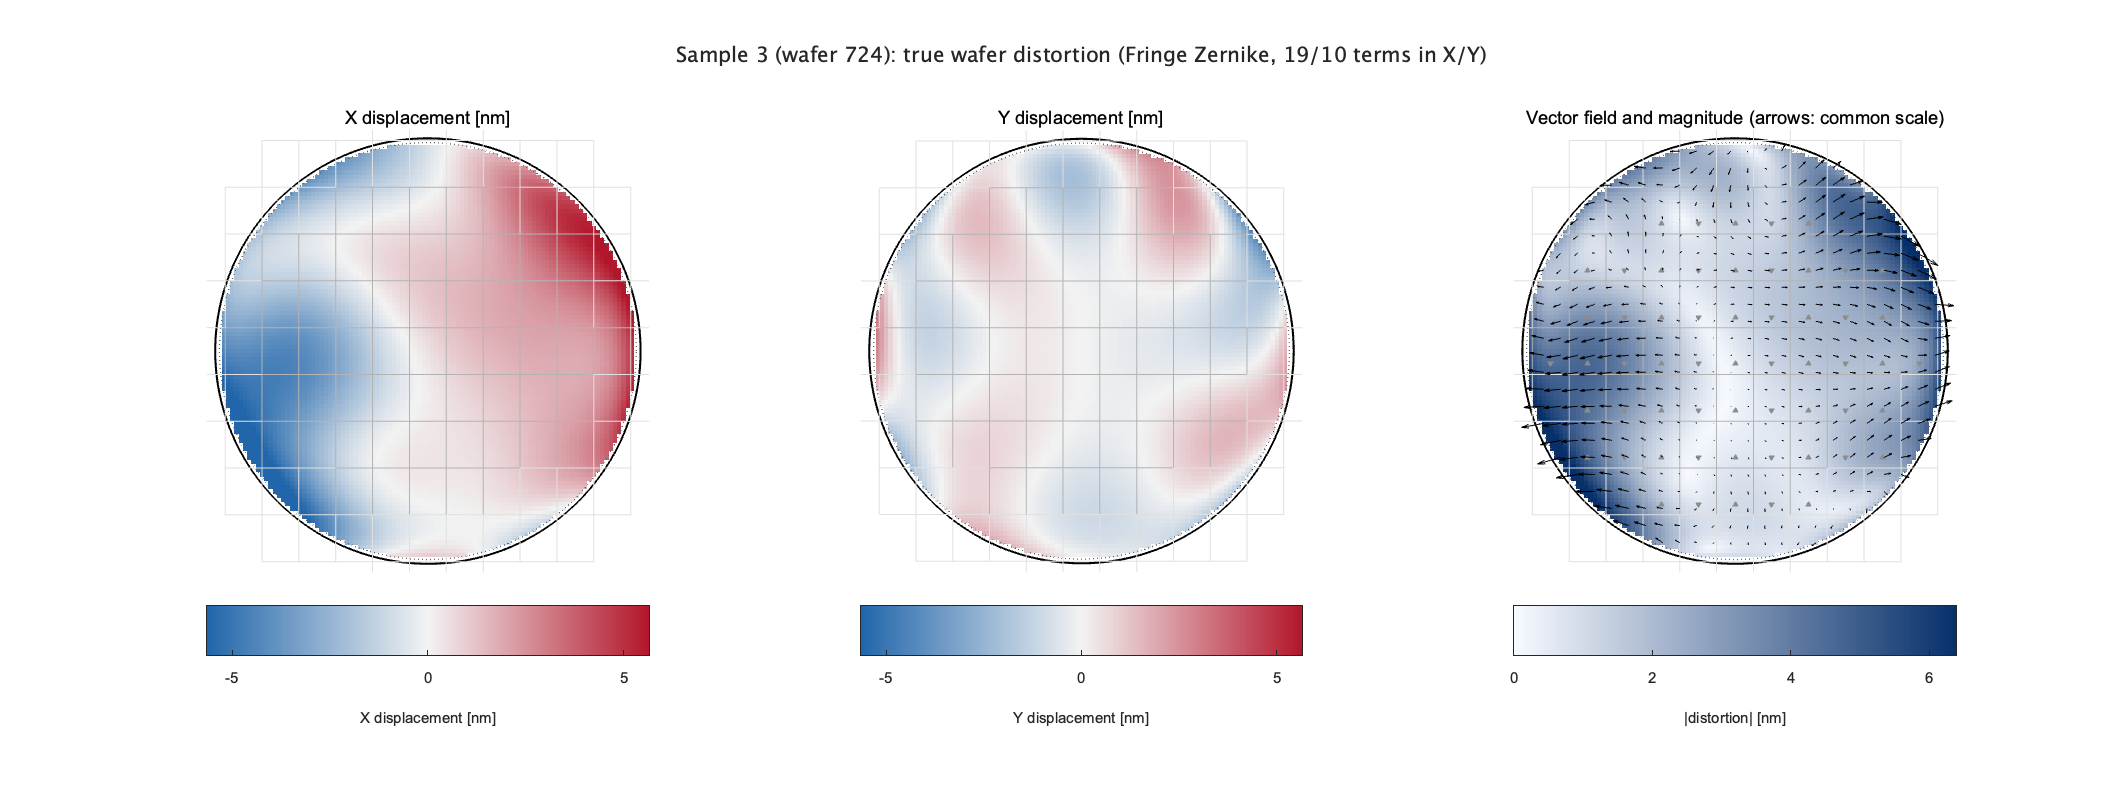
\includegraphics[width=0.92\textwidth]{A1_sample3_truth.png}
  \caption{Sample 3 の真の面内傾向．}
\end{figure}

\subsubsection*{sampling map}
\begin{figure}[H]
  \centering
  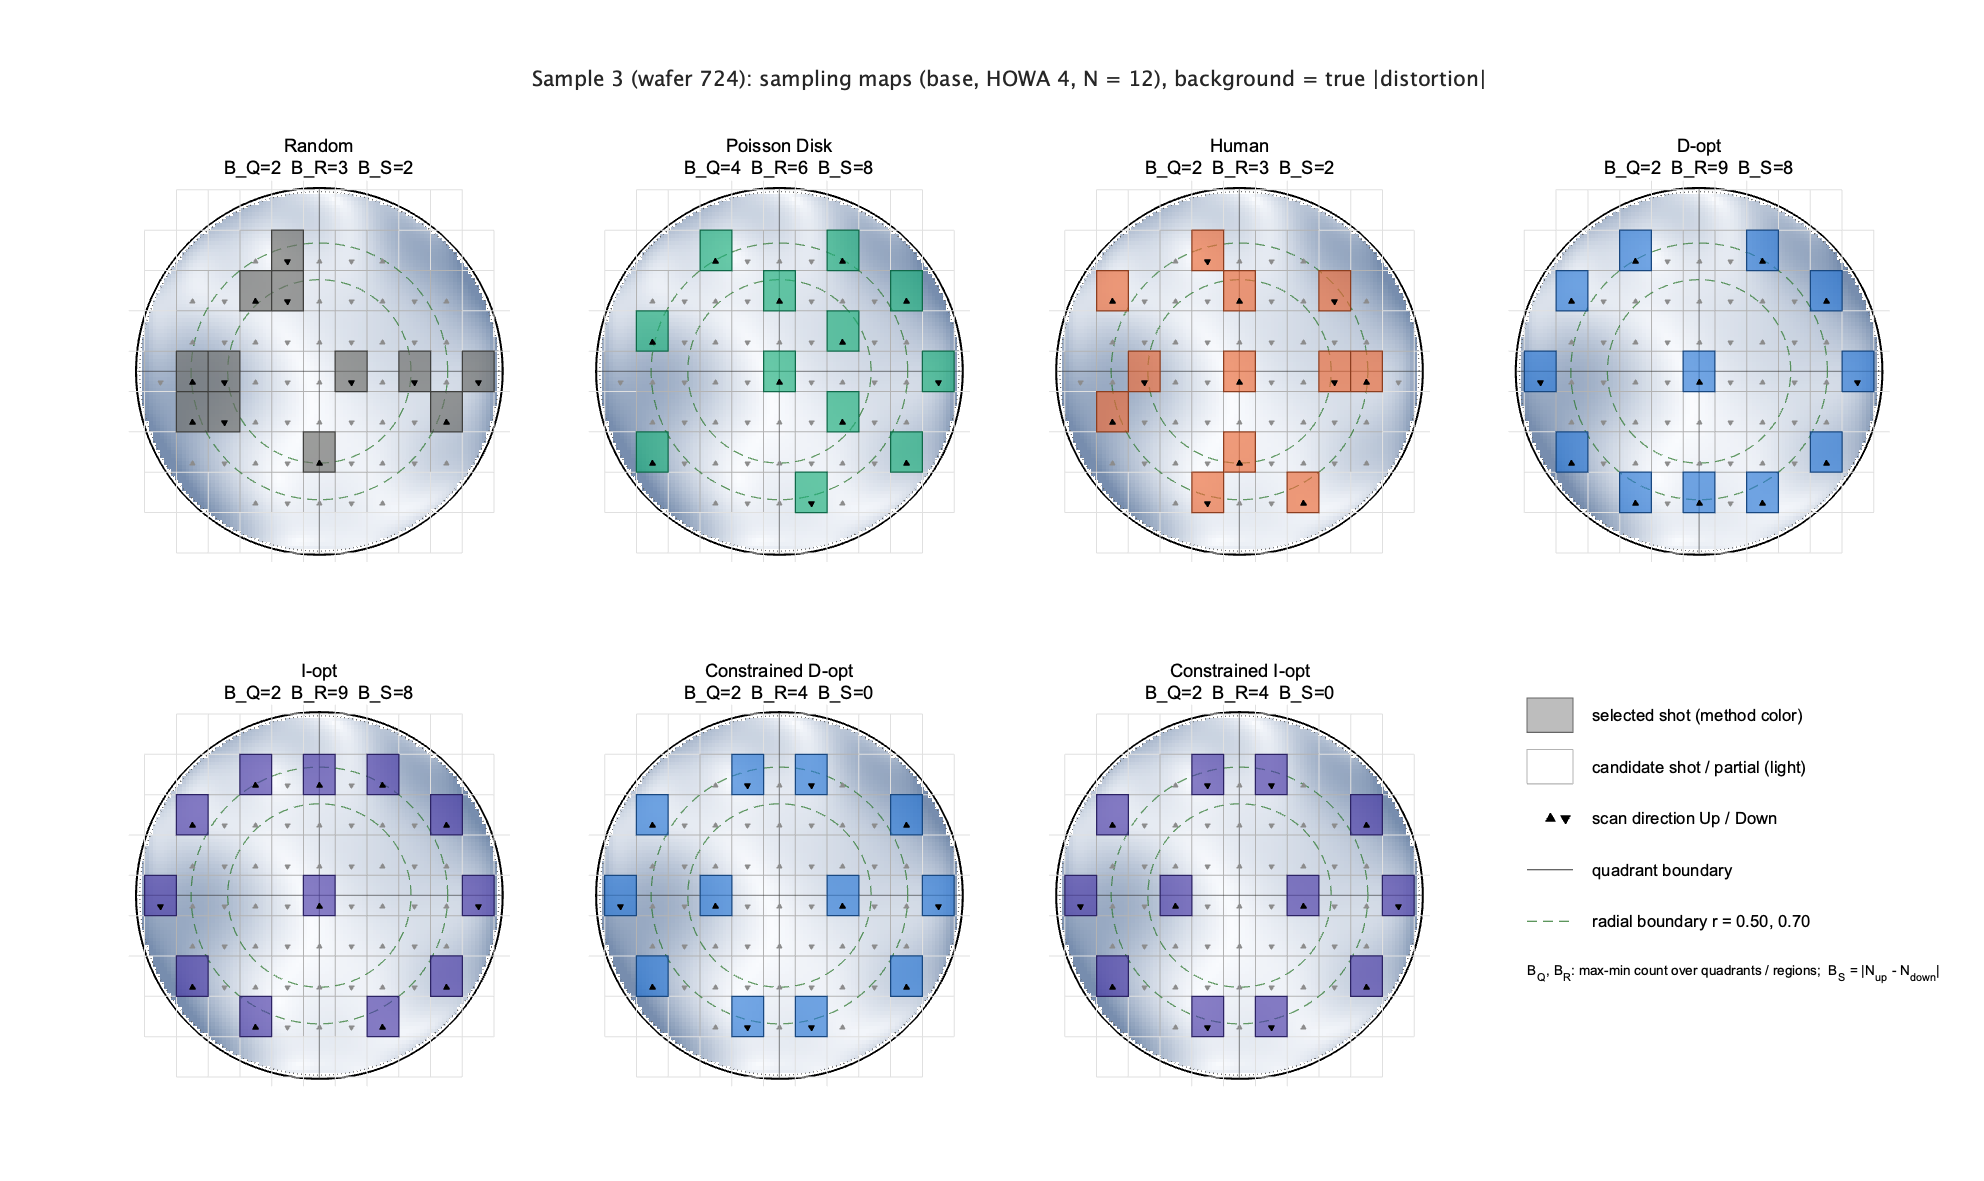
\includegraphics[width=0.85\textwidth]{A2_sample3_sampling_base.png}
  \caption{Sample 3 の sampling map（HOWA 4次，$N=12$）．}
\end{figure}

\subsubsection*{補正後残差vector field}
\begin{figure}[H]
  \centering
  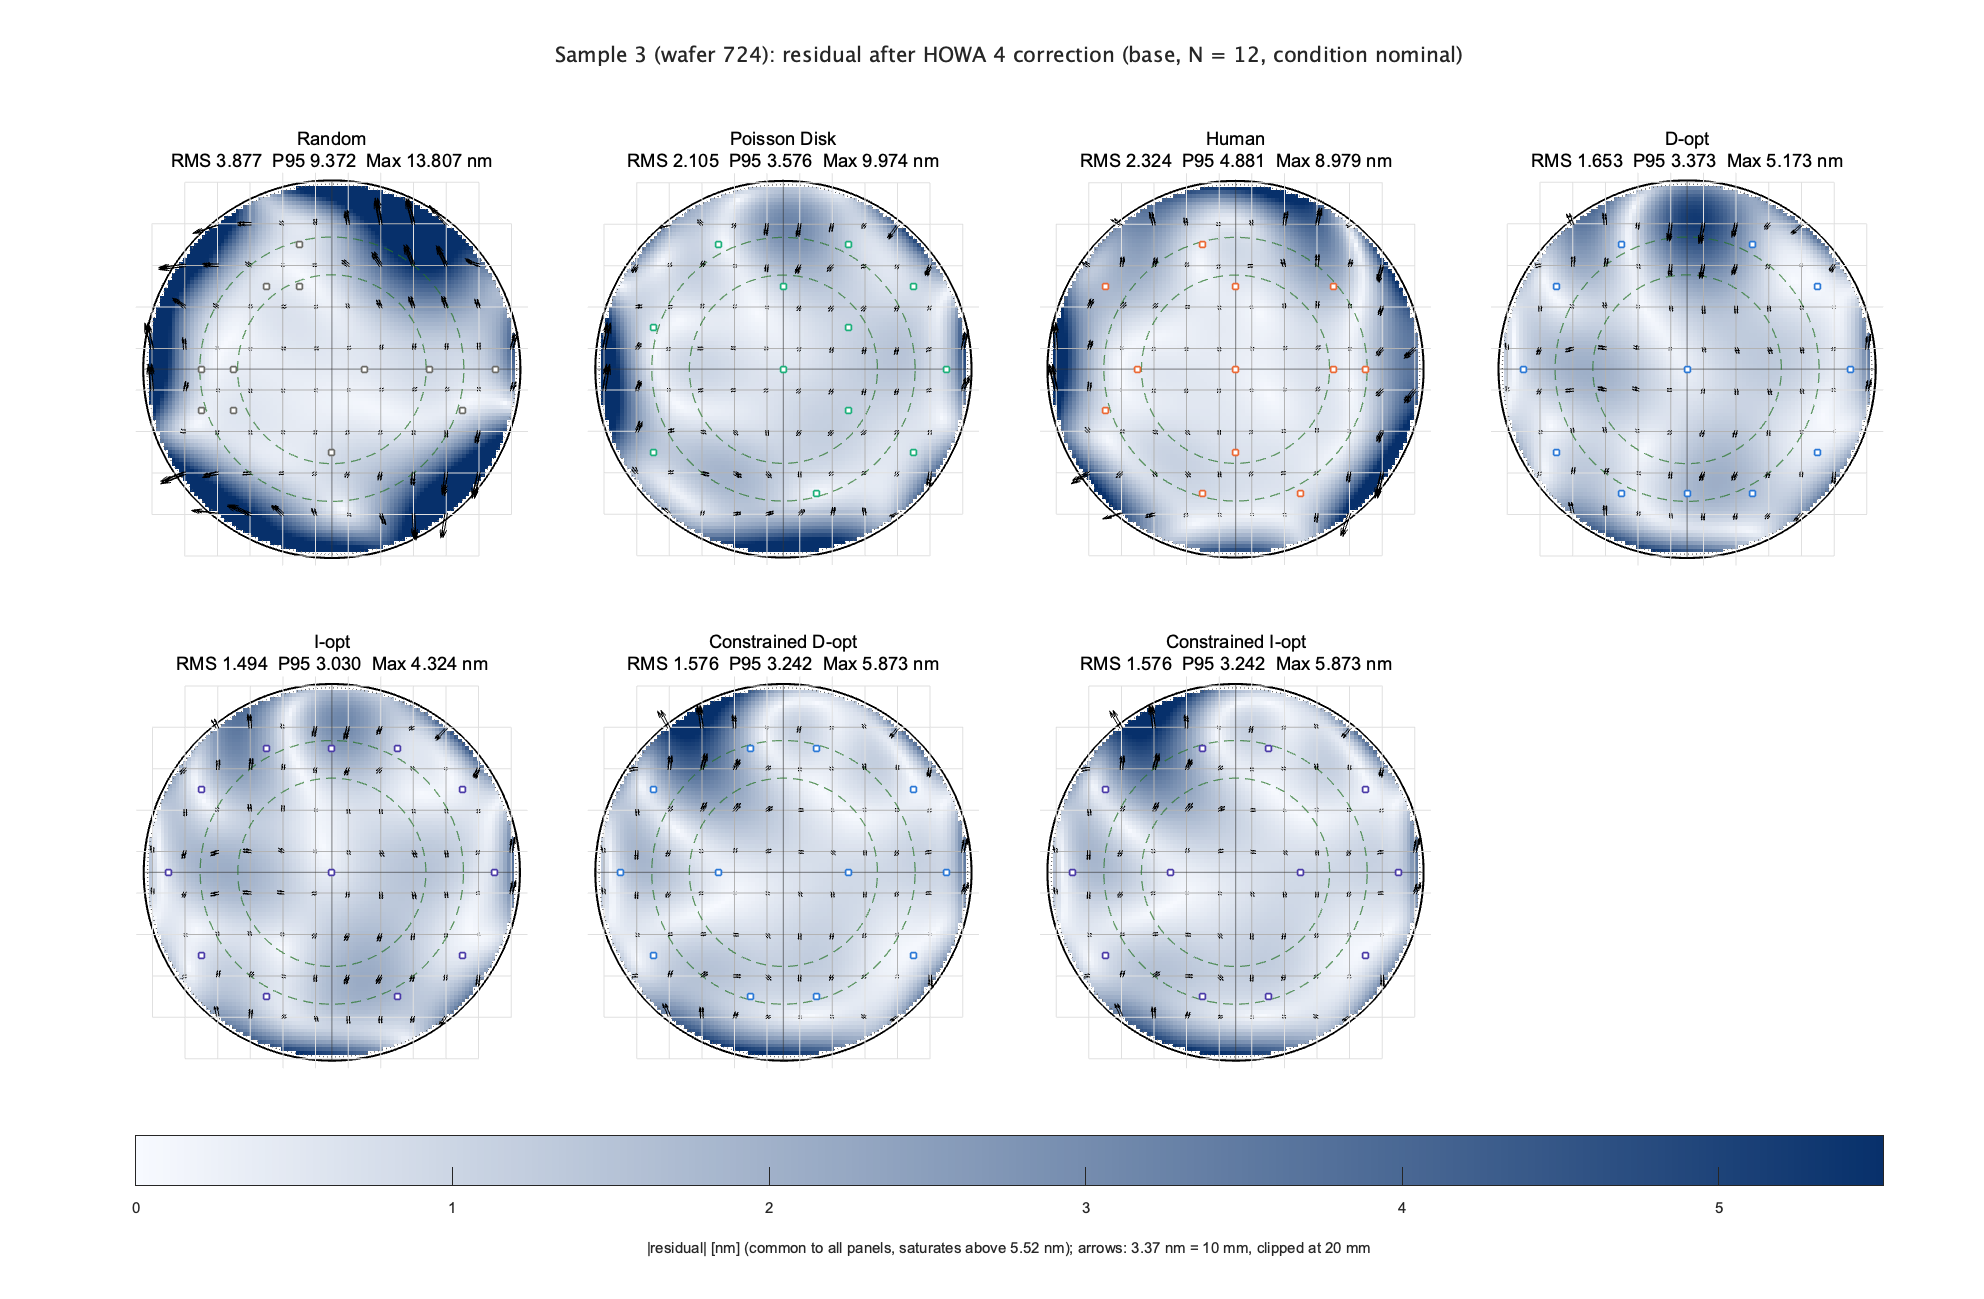
\includegraphics[width=0.85\textwidth]{A3_sample3_residual_base.png}
  \caption{Sample 3 のHOWA 4次補正後の残差．}
\end{figure}

Sample 3は，どの手法でも残差が大きいwaferである．
HOWA 4次で表せない成分が大きく（モデル不一致の下限0.97\,nm，1000 waferの平均0.55\,nm），最良のI-optでも1.49\,nm，C-D-opt 1.58，D-opt 1.65，Poisson 2.10，Human 2.32\,nmだった．
このようなwaferでは，計測shotの配置より補正モデルの次数（表現力）が残差を決めており，sampling最適化の効果は相対的に小さい．


\clearpage
\subsection{強制計測shotありの例（Sample 1）}

\begin{figure}[H]
  \centering
  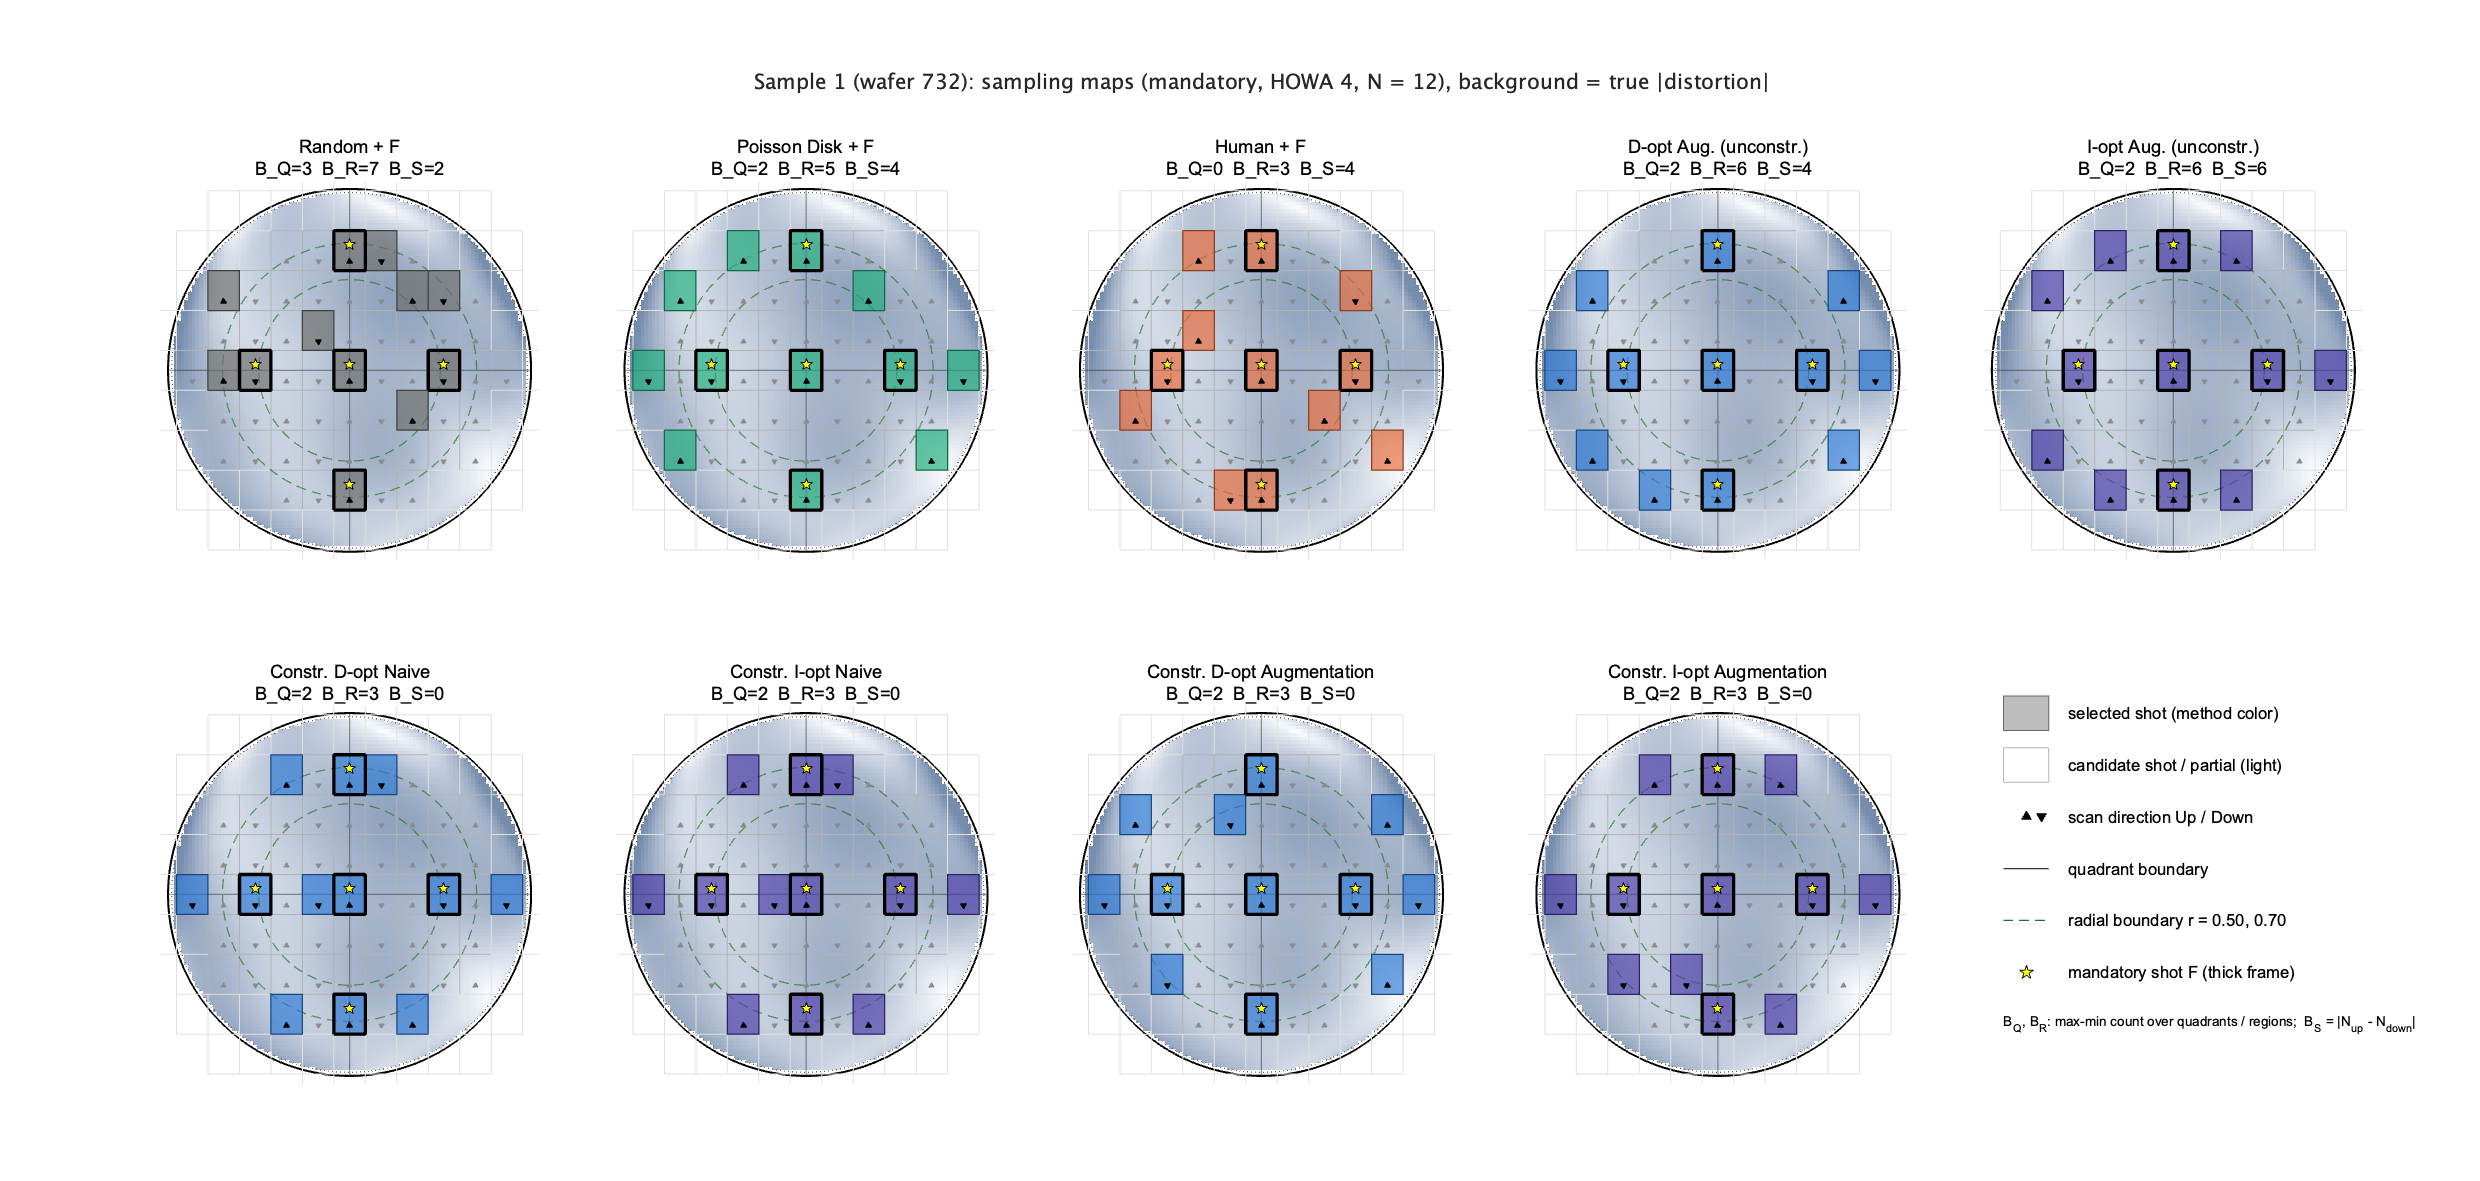
\includegraphics[width=0.85\textwidth]{A2_sample1_sampling_mandatory.png}
  \caption{Sample 1，強制計測shotありの sampling map（HOWA 4次，$N=12$，☆と太枠が強制計測shot）．}
\end{figure}

\begin{figure}[H]
  \centering
  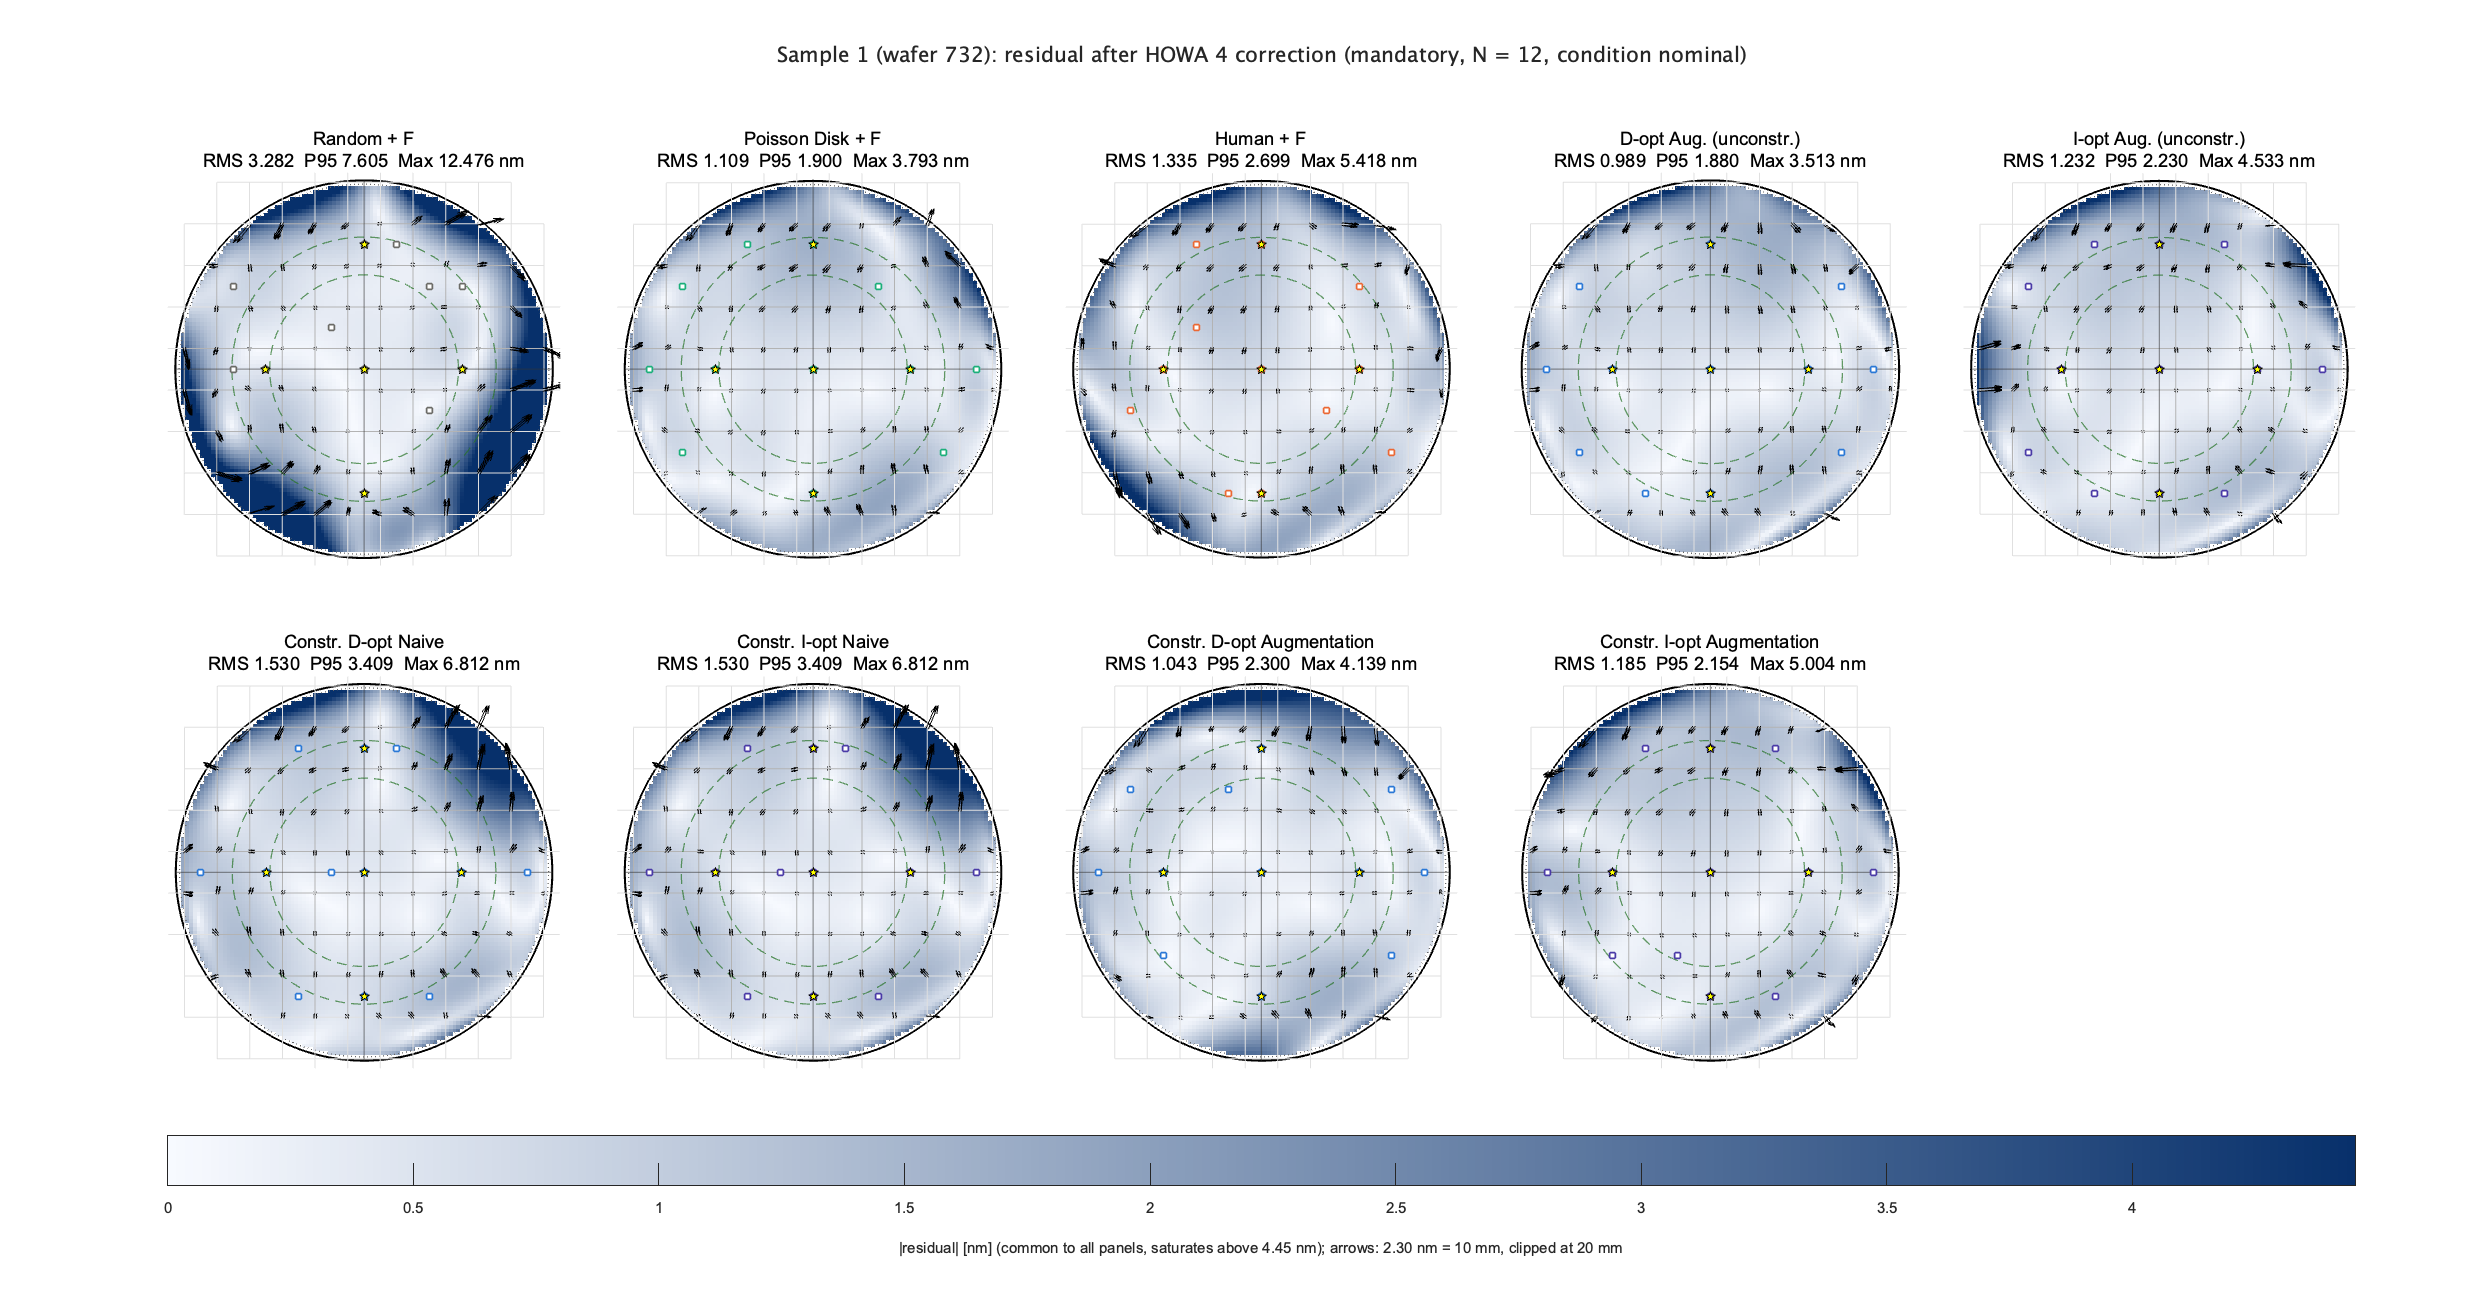
\includegraphics[width=0.85\textwidth]{A3_sample1_residual_mandatory.png}
  \caption{Sample 1，強制計測shotありのHOWA 4次補正後の残差．}
\end{figure}

強制計測shot（中心と十字の5 shot）を含む同じwafer・同じshot数（12）では，C-D-opt Augmentation 1.04\,nm，C-I-opt Augmentation 1.19，素朴な方法（Naive，C-D・C-Iとも）1.53，制約なしの拡張計画（D-opt Aug）0.99，Human+F 1.33\,nmだった．
Augmentationは，強制shotがすでにある中心付近を避けて残りのshotを外周と斜め方向に配置しているのに対し，Naiveは強制shotのすぐ隣（x軸上のInner領域）にもshotを置いており，情報が重複している．



\end{document}
